% siminos/gudorf/thesisProposal/proposal.tex
% $Author: mgudorf3 $ $Date: 2019-01-12 05:27:53 -0500 (Sat, 12 Jan 2019) $

%%%%%%%%%%%%%%%%%%%%%%%%%%%%%%%%%%%%%%%%%%%%%%%%%%%%%%%%%%%%%%%%%%%%%%
            \newif\ifpaper \newif\ifPDF \newif\ifboyscout
            %\newif\ifOUP \newif\ifdasbuch \newif\ifarticle
            %\newif\ifsolutions
            \boyscouttrue\PDFtrue\paperfalse
%%%%%% hyperlinked PDF version:
 \boyscouttrue  % commented, internal version
%  \boyscoutfalse % public
%%%%%% uncomment to generate paper B&W pdf for GaTech thesis submission:
%  \papertrue\boyscoutfalse

\documentclass[reqno,11pt,oneside]{article}

\usepackage[top=1in, bottom=1.2in, left=1.25in, right=1.25in]{geometry}
\usepackage[intlimits]{amsmath} % Puts the limits of integrals on top and bottom
\usepackage{amsxtra}     % Use various AMS packages
\usepackage{amsthm}
\usepackage{amssymb}
\usepackage{amsfonts}
\usepackage{ifthen}
\usepackage[font=small,labelfont=bf]{caption}
\usepackage{subcaption}
%%%%%%%%%%%%%%%%%%%%%%%%%%%%%%%%%%%%%%%%%%%%%%%%%%%%%%%%%%%%%%%%%%%%%%%%%%%%%%
\ifPDF %%%%%%%% HYPERLINKED VS PAPER PDF VERSIONS %%%%%%%%%%%%%%%%%%%%
   \usepackage[pdftex]{graphicx} % test switch to pdflatex?
  \ifpaper % prepare public B&W pdf individual chapters:
    \newcommand{\color}[1]{}
  \else    % prepare hyperlinked WWW/chapters/ChaosBook.pdf
    \usepackage[pdftex]{color}
            %% pdfmark produces Acroread index:
    \usepackage[pdfauthor={Matthew Gudorf}% must be LAST package loaded
                pdftitle={Just do it: Kuramoto-Sivashinsky state space},%
                pdftex,colorlinks]{hyperref} %% hyperlinks
            %% TEMPORARILY COMMENTED OUT backref:
    %       pdfmark,colorlinks,backref]{hyperref}
  \fi
%%%%%%%%%%%%%%%%%%%%%%%%%%%%%%%%%%%%%%%%%%%%%%%%%%%%%%%%%%%%%%%%%%%%%%%%%%%%%%


\graphicspath{{../../figs/ksstFigs/}
              {../../figs/}}

\newcounter{chapter}

% dasbuch/book/inputs/def.tex
% $Author: predrag $ $Date: 2021-07-23 16:15:21 -0400 (Fri, 23 Jul 2021) $

%%%%%%%%%%%%%%%%%%%%%%%%%%%%%%%%%%%%%%%%%%%%%%%%%%%%%%%%%%%%%%%%%%%%%%%%%
%% defines macros used throughout ChaosBook and related
%%%%%%%%%%%%%%%%%%%%%%%%%%%%%%%%%%%%%%%%%%%%%%%%%%%%%%%%%%%%%%%%%%%%%%%%%

%               Predrag         17dec2020
%               Predrag         23may2020
%               Predrag          6oct2017
% \input{inputs/defBtracks} after def.tex to pdfLaTeX birdtracks macros
%               Predrag         11apr2015
% collected group theoretic macros
%               Predrag         25jan2014
% defined graphicspath
%               Predrag         15sep2013
% \goodbreak arXiv -> arXiv
%               Predrag         27feb2012
%               Predrag         17feb2012
%               Predrag          4feb2012
%               Predrag          9oct2009
%               Predrag         12jun2008
%               Predrag         15dec2008
%               Predrag         29oct2005
%               Predrag         13jul2005
%               Predrag         24apr2005
%               Predrag         14feb2005
%               Predrag         22jan2005
%               Predrag         16nov2004
%               Predrag         13jun2004
%               Predrag          3may2004
%               Predrag         10apr2004
%               Predrag         21feb2004
%               Predrag          4oct2003
%               Predrag         30aug2003
%               Predrag         20jun2003
%               Predrag         17jan2003
%               Predrag          6dec2002
%               Predrag          7jul2002
%               Predrag         19nov2000
%               Ronnie          23sep2000
% Predrag disabled \basedirectory machine identifier    25aug2000
% Predrag created               30oct1994

    %%%%%%% CL18 specific %%%%%%%%%%%%%%%%%%%%%%%%%%%%
\newcommand{\fundPip}{fundamental parallelepiped}
\newcommand{\brick}{block}
\newcommand{\Brick}{Block}
\newcommand{\jacobianOrb}{orbit Jacobian matrix}
\newcommand{\JacobianOrb}{Orbit Jacobian matrix}
\newcommand{\jacobianOrbs}{orbit Jacobian matrices}
\newcommand{\JacobianOrbs}{Orbit Jacobian matrices}
\newcommand{\HillDet}{Hill determinant}
\newcommand{\PV}{Percival-Vivaldi}
\newcommand{\AW}{Adler-Weiss}
% \newcommand{\GO}{Gutkin-Osipov}
\newcommand{\SLn}[2]{\ensuremath{\textrm{SL}_{#1}(#2)}}
\newcommand{\jMorb}{{\ensuremath{\cal \jMps}}}
\newcommand{\conf}{\ensuremath{x}}      % Configuration space coordinate
\newcommand{\lattice}{\ensuremath{\mathcal{L}}}
\newcommand{\jMat}{\mathbb{\jMps}}

    %%%%%% Boris definitions  %%%%%%%%%%%%%%%%%%%%%%%%%%%%
\newcommand{\Aa}{\ensuremath{\bar{\A}}}         % alphabet with a bar
\newcommand{\A}{\ensuremath{\mathcal{A}}}       % alphabet
% \newcommand{\Ai}{\ensuremath{\mathcal{A}_0}}    % alphabet inner
% \newcommand{\Ae}{\ensuremath{\mathcal{A}_1}}    % alphabet outer
% \newcommand{\R}{\ensuremath{\mathcal{R}}}
% \newcommand{\m}{\ensuremath{\mathsf{m}}}     % Boris
% \newcommand{\m}{\ensuremath{m}}     % Predrag experimental 2016-11-08
\newcommand{\Mm}{\ensuremath{\mathsf{M}}}
% \newcommand{\MmR}{\Mm_\R}
\newcommand{\Xx}{\ensuremath{\mathsf{X}}}
% \newcommand{\Zz}{\ensuremath{\mathbb{Z}^2}}
% \newcommand{\Spshift}{\mathrm{S}}
% \newcommand{\Tshift}{\mathrm{T}}
% \newcommand{\Pol}{\mathcal{P}}                  % Boris
% \newcommand{\ZLT}{\mathbb{Z}^2_{\scriptscriptstyle\mathrm{LT}}}
%\newcommand{\q}{\ensuremath{\mathsf{m}}}     % Boris
% \newcommand{\q}{\ensuremath{q}}     % Predrag experimental 2016-11-08
% \newcommand{\D}{\mathcal{D}}
% \newcommand{\gd}{\mathsf{g}}
% \newcommand{\gp}{\mathsf{g}^0}


\ifpaper % prepare for B&W paper printing:
       \newcommand{\href}[2]{{#2}}  % no hyperref
       \newcommand{\HREF}[2]{{#2}}
       \renewcommand{\color}[1]{}       % B&W
       \newcommand{\wwwcb}[1]{{ChaosBook.org#1}}
       \newcommand{\wwwgt}{{birdtracks.eu}}
       \newcommand{\wwwQFT}[1]{{ChaosBook.org/\-Field\-Theory#1}}
       \newcommand{\wwwcnsQFT}[1]{{ChaosBook.org/\-Field\-Theory#1}}
       \newcommand{\weblink}[1]{{#1}}
       \newcommand{\arXiv}[1]{{arXiv:#1}}
       \newcommand{\bioRxiv}[1]{{bioRxiv:#1}}
       \newcommand{\mpArc}[1]{{mp\_arc~#1}}
\else % prepare hyperlinked pdf
        \newcommand{\wwwcb}[1]{       % keep homepage flexible:
                  {\href{http://ChaosBook.org#1}
              {ChaosBook.org#1}}}
       \newcommand{\wwwgt}{{\href{http://birdtracks.eu}
              {birdtracks.eu}}}
       \newcommand{\wwwQFT}[1]{
                  {\href{http://ChaosBook.org/FieldTheory#1}
              {ChaosBook.org/\-Field\-Theory#1}}}
       \newcommand{\wwwcnsQFT}[1]{
                  {\href{http://ChaosBook.org/FieldTheory#1}
              {ChaosBook.org/\-Field\-Theory#1}}}
       \newcommand{\weblink}[1]{{\href{http://#1}{#1}}}
       \newcommand{\HREF}[2]{
              {\href{#1}{#2}}}
       \newcommand{\mpArc}[1]{
              {\href{http://www.ma.utexas.edu/mp_arc-bin/mpa?yn=#1}
                   {mp\_arc~#1}}}
       \newcommand{\arXiv}[1]{
              {\href{https://arXiv.org/abs/#1}{arXiv:#1}}}
       \newcommand{\bioRxiv}[1]{
              {\href{https://biorxiv.org/content/10.1101/#1}{bioRxiv:#1}}}
\fi

%%%%%%%%%%%%%%%%%%%%%% QUOTATIONS %%%%%%%%%%%%%%%%%%%%%%%%%%%%%%%%%%%%%%
%
%  the learned/witty quotes at the chapter and section headings
%
\newsavebox{\bartName}
\newcommand{\bauthor}[1]{\sbox{\bartName}{\parbox{\textwidth}{\vspace*{0.8ex}
       %\hspace*{\fill}
       \hspace{2em}---\small\noindent #1}}}
\newenvironment{bartlett}{\hfill\begin{minipage}[t]{0.65\textwidth}\small}%
{\hspace*{\fill}\nolinebreak[1]\usebox{\bartName}\vspace*{1ex}\end{minipage}}
%
%  a quotation inserted into the text
%
\newenvironment{txtquote}{\begin{quotation} \small}{\end{quotation}}

\newcommand{\student}{Henriette Roux}
%\newcommand{\student}{Jens J. Jensen}

%%%%%%%%%%%%%%%%%%%%%% INDEXING %%%%%%%%%%%%%%%%%%%%%%%%%%%%%%%%%%%%%%%%%
\newcommand{\indx}[1] {#1\index{#1}}    % do not need to repeat the word

\newcommand{\file}[1]{$\footnotemark\footnotetext{{\bf file} #1}$}
% PC 9sep2008 commented out (is it used?):
%\newcommand{\lecture}[2]{ \addtocontents{toc}
%           {{\scriptsize #1}{\sf\small lecture: \scriptsize #2}} }

%%%%%%%%%%%%%%% EQUATIONS %%%%%%%%%%%%%%%%%%%%%%%%%%%%%%%
\newcommand{\beq}{\begin{equation}}
\newcommand{\continue}{\nonumber \\ }
\newcommand{\nnu}{\nonumber}
\newcommand{\eeq}{\end{equation}}
\newcommand{\ee}[1] {\label{#1} \end{equation}}
\newcommand{\bea}{\begin{eqnarray}}
\newcommand{\ceq}{\nonumber \\ & & }
\newcommand{\eea}{\end{eqnarray}}
\newcommand{\barr}{\begin{array}}
\newcommand{\earr}{\end{array}}

%%%%%%%%%%%%%%% REFERENCING EQUATIONS ETC. %%%%%%%%%%%%%%%%%%%%%%%%%%%%%%%
\newcommand{\rf}     [1] {~\cite{#1}}
\newcommand{\refref} [1] {ref.~\cite{#1}}
\newcommand{\refRef} [1] {Ref.~\cite{#1}}
\newcommand{\refrefs}[1] {refs.~\cite{#1}}
\newcommand{\refRefs}[1] {Refs.~\cite{#1}}
\newcommand{\refeq}  [1] {(\ref{#1})}
            % in amstex, \eqref is predefined and better than \refeq
\newcommand{\refeqs} [2]{(\ref{#1}--\ref{#2})}
\newcommand{\refpage}[1] {page~\pageref{#1}}
\newcommand{\reffig} [1] {figure~\ref{#1}}
\newcommand{\reffigs} [2] {figures~\ref{#1} and~\ref{#2}}
\newcommand{\refFig} [1] {Figure~\ref{#1}}
\newcommand{\refFigs} [2] {Figures~\ref{#1} and~\ref{#2}}
\newcommand{\reftab} [1] {table~\ref{#1}}
\newcommand{\refTab} [1] {Table~\ref{#1}}
\newcommand{\reftabs}[2] {tables~\ref{#1} and~\ref{#2}}
\newcommand{\refsect}[1] {sect.~\ref{#1}}
\newcommand{\refsects}[2] {sects.~\ref{#1} and \ref{#2}}
\newcommand{\refSect}[1] {Sect.~\ref{#1}}
\newcommand{\refSects}[2] {Sects.~\ref{#1} and \ref{#2}}
\newcommand{\refsecttosect}[2] {Sects.~\ref{#1} to~\ref{#2}}
\newcommand{\refchap}[1] {chapter~\ref{#1}}
\newcommand{\refChap}[1] {Chapter~\ref{#1}}
\newcommand{\refchaps}[2] {chapters~\ref{#1} and~\ref{#2}}
\newcommand{\refchaptochap}[2] {chapters~\ref{#1} to~\ref{#2}}
\newcommand{\refappe}[1] {appendix~\ref{#1}}
\newcommand{\refappes}[2] {appendices~\ref{#1} and~\ref{#2}}
\newcommand{\refAppe}[1] {Appendix~\ref{#1}}
\newcommand{\refrem} [1] {remark~\ref{#1}}
\newcommand{\refRem} [1] {Remark~\ref{#1}}
\newcommand{\refexam}[1] {example~\ref{#1}}
\newcommand{\refExam}[1] {Example~\ref{#1}}
\newcommand{\refexer}[1] {exercise~\ref{#1}}
\newcommand{\refExer}[1] {Exercise~\ref{#1}}
\newcommand{\refsolu}[1] {solution~\ref{#1}}
\newcommand{\refSolu}[1] {Solution~\ref{#1}}

%%%%%%%%%%%%%%  Abbreviations %%%%%%%%%%%%%%%%%%%%%%%%%%%%%%%%%%%%%%%%
%%% APS (American Physiology Society, it seems) style:
%%%     Latin or foreign words or phrases should be roman, not italic.
%%%     Insert a `hard' space after full points
%%%                                         that do not end sentences.

\newcommand{\etc}{{etc.}}       % APS
\newcommand{\etal}{{\em et al.}}    % etal in italics, APS too
\newcommand{\ie}{{i.e.}}        % APS
\newcommand{\cf}{{\em cf.\ }}     % APS
\newcommand{\eg}{{e.g.\ }}        % APS, OUP, hard space '\eg\ NextWord'
% \newcommand{\etc}{{\em etc.}}     % etcetera in italics
% \newcommand{\ie}{{that is}}       % use Latin or English?  Decide later.
% \newcommand{\cf}{{cf.}}
% \newcommand{\eg}{{\it e.g.,\ }}   % Wirzba 2sep2001

%%%%%%%%%%%%%%% ChaosBook Abbreviations %%%%%%%%%%%%%%%%%%%%%%%%

\newcommand{\evOper}{evolution oper\-ator}
\newcommand{\EvOper}{Evolution oper\-ator}
 %% \newcommand{\evOp}{Ruelle operator} %could be ``evolution'' instead?
%\newcommand{\FPoper}{Frobenius-Perron oper\-ator}
\newcommand{\FPoper}{Perron-Frobenius oper\-ator} % Pesin's ordering
\newcommand{\FP}{Perron-Frobenius}
\newcommand{\statesp}{state space}
\newcommand{\Statesp}{State space}
\newcommand{\stateDsp}{state-space}
\newcommand{\StateDsp}{State-space}
\newcommand{\fixedpnt}{fixed point}
\newcommand{\Fixedpnt}{fixed point}
\newcommand{\maslov}{topological}
\newcommand{\Maslov}{Topological}
%\newcommand{\Maslov}{Keller-Maslov}
\newcommand{\jacobian}{Jacobian}        % determinant
% \newcommand{\jacobianM}{fundamental matrix} % no known standard name?
% \newcommand{\jacobianMs}{fundamental matrices}  %
% \newcommand{\JacobianM}{Fundamental matrix} %
% \newcommand{\JacobianMs}{Fundamental matrices}  %
\newcommand{\jacobianM}{Jacobian matrix}  % back to Predrag's name 20oct2009
\newcommand{\jacobianMs}{Jacobian matrices}   % matrices
\newcommand{\JacobianM}{Jacobian matrix} %
\newcommand{\JacobianMs}{Jacobian matrices}  %
\newcommand{\FloquetM}{Floquet matrix} % specialized to periodic orb
\newcommand{\FloquetMs}{Floquet matrices}  %
% \newcommand{\stabmat}{matrix of variations}   % Arnold, says Vattay
\newcommand{\stabmat}{stability matrix}     % stability matrix, velocity gradients
\newcommand{\Stabmat}{Stability matrix}     % Stability matrix
\newcommand{\stabmats}{stability matrices}
\newcommand{\monodromyM}{monodromy matrix} % monodromy matrix, Poincare cut
\newcommand{\MonodromyM}{Monodromy matrix} % monodromy matrix, Poincare cut
\newcommand{\dzeta}{dyn\-am\-ic\-al zeta func\-tion}
\newcommand{\Dzeta}{Dyn\-am\-ic\-al zeta func\-tion}
\newcommand{\tzeta}{top\-o\-lo\-gi\-cal zeta func\-tion}
\newcommand{\Tzeta}{Top\-o\-lo\-gi\-cal zeta func\-tion}
\newcommand{\BERzeta}{BER zeta func\-tion}
%\newcommand{\tzeta}{Artin-Mazur zeta func\-tion} %alternative to topological
\newcommand{\qS}{semi\-classical zeta func\-tion}
%\newcommand{\qS}{Gutz\-willer-Voros zeta func\-tion}
\newcommand{\Gt}{Gutz\-willer trace formula}
\newcommand{\Fd}{spec\-tral det\-er\-min\-ant}
%\newcommand{\fd}{spec\-tral det\-er\-min\-ant} %in many articles
\newcommand{\FD}{Spec\-tral det\-er\-min\-ant}
\newcommand{\cFd}{semiclass\-ic\-al spec\-tral det\-er\-mi\-nant}
\newcommand{\cFD}{Semiclass\-ic\-al spec\-tral det\-er\-mi\-nant}
% \newcommand{\cFd}{semiclass\-ic\-al Fred\-holm det\-er\-mi\-nant}
\newcommand{\Vd}{Vattay det\-er\-mi\-nant}
\newcommand{\cycForm}{cycle averaging formula}
\newcommand{\CycForm}{Cycle averaging formula}
\newcommand{\freeFlight}{mean free flight time}
\newcommand{\FreeFlight}{Mean free flight time}
\newcommand{\pdes}{partial differential equations}
\newcommand{\Pdes}{Partial differential equations}
% \newcommand{\dof}{dof}         % Hamiltonian deegree of freedom
\newcommand{\dof}{degree of freedom}
% \newcommand{\Dof}{Degree of freedom}
\newcommand{\dofs}{degrees of freedom}
% \newcommand{\Dofs}{Degrees of freedom}
\newcommand{\cdof}{computational degree of freedom}
\newcommand{\Cdof}{Computational degree of freedom}
\newcommand{\cdofs}{computational degrees of freedom}
\newcommand{\Cdofs}{Computational degrees of freedom}

%%%%%%%%%%%%%%% VECTORS, MATRICES, NORMS %%%%%%%%%%%%%%%%%%%%%%%%%%%%%%%%%

	% without large brackets:
\newcommand{\braket}[2]
		   {\langle{#1}\vphantom{#2}|\vphantom{#1}{#2}\rangle}
\newcommand{\bra}[1]{\langle{#1}\vphantom{ }|}
\newcommand{\ket}[1]{|\vphantom{}{#1}\rangle}
	% with large brackets:
%\newcommand{\bra}[1]{\left\langle{#1}\vphantom{ }\right|}
%\newcommand{\ket}[1]{\left|\vphantom{}{#1}\right\rangle}
%\newcommand{\braket}[2]{\left\langle{#1}
%                        \vphantom{#2}\right|\left.\vphantom{#1}
%                        {#2}\right\rangle}

\newcommand{\dual}[1]{{#1}^\dag}
% \newcommand{\dual}[1]{{#1}^\ast}
% \newcommand{\transp}[1]{\bar{#1}}
% \newcommand{\transp}[1]{{#1}{}^T}
\newcommand{\transp}[1]{{#1}{}^\top}

% Commented out AMS-style pmatrix, which is incompatible with TeX/LaTeX pmatrix
% used throughout dasbuch. Fri Oct 12 15:51:03 EDT 2007

\newcommand{\MatrixII}[4]{\left[
\begin{array}{cc}
{#1}  &  {#2} \\
{#3}  &  {#4} \end{array} \right]}
% a problem with \pmatrix 12oct 2007
%\newcommand{\MatrixII}[4]{
%   \begin{bmatrix}{#1}  &  {#2} \\
%                  {#3}  &  {#4} \end{bmatrix}}

\newcommand{\MatrixIII}[9]{
\begin{bmatrix}
  {#1}  &  {#2} &  {#3} \\
  {#4}  &  {#5} &  {#6} \\
  {#7}  &  {#8} &  {#9}
\end{bmatrix}
          }

\newcommand{\transpVectorII}[2]{
    \begin{bmatrix}{#1}  &  {#2}  \end{bmatrix}}

%\newcommand{\VectorII}[2]{\left(
%\begin{array}{cc}
%{#1}  &  {#2} \end{array} \right)}
%
%\newcommand{\VectorII}[2]{
%  \pmatrix{ {#1} \cr {#2}}
%}

 \newcommand{\VectorII}[2]{
    \begin{bmatrix} {#1} \\
                    {#2}  \end{bmatrix}}

 \newcommand{\VectorIII}[3]{
    \begin{bmatrix} {#1} \\
                    {#2} \\
                    {#3} \end{bmatrix}}

%\newcommand{\transpVectorII}[2]{\left(
%\begin{array}{c}
%   {#1} \cr
%   {#2}\end{array} \right)
%}

%\newcommand{\VectorIII}[3]{
%  \pmatrix{ {#1} \cr
%            {#2} \cr
%            {#3}
%          }
%}

\newcommand{\combinatorial}[2]{ {#1 \choose #2}}

%%%%%%%%%%%%%%% Sundry symbols within math eviron.: %%%%%%%%%%%%

\newcommand{\obser}{\ensuremath{a}}     % an observable from phase space to R^n
\newcommand{\Obser}{\ensuremath{A}}     % time integral of an observable
\newcommand{\onefun}{\iota} % the function that returns one no matter what
\newcommand{\defeq}{=}      % the different equal for a definition
\newcommand {\deff}{\stackrel{\rm def}{=}}
\newcommand{\reals}{\mathbb{R}}
\newcommand{\complex}{\mathbb{C}}
\newcommand{\integers}{\mathbb{Z}}
\newcommand{\rationals}{\mathbb{Q}}
\newcommand{\naturals}{\mathbb{N}}
\newcommand{\LieD}{{\mathcal{L}\!\!\llap{-}\,\,}}  % {{\pound}} % Lie Derivative
\newcommand{\half}{{\scriptstyle{\frac{1}{2}}}}
\newcommand{\pde}{\partial}
\newcommand{\pdfrac}[2]{\frac{\partial #1}{\partial #2}}
\renewcommand\Im{\ensuremath{\mathrm{Im}\,}}
\renewcommand\Re{\ensuremath{\mathrm{Re}\,}}
\renewcommand{\det}{\mathrm{det}\,}
\newcommand{\Det}{\mathrm{Det}\,}
\newcommand{\tr}{\mathrm{tr}\,}
\newcommand{\Tr}{\mathrm{Tr}\,}
\newcommand{\trDiscr}[2]{\Cn{#1}^{#2}}  % Xiong Ding
\newcommand{\sign}[1]{\sigma_{#1}}
%\newcommand{\sign}[1]{{\rm sign}(#1)}
\newcommand{\mInv}{{I}}                 % material invariant
\newcommand{\msr}{\ensuremath{\rho}}                % measure
\newcommand{\Msr}{{\mu}}                % coarse measure
\newcommand{\dMsr}{{d\mu}}              % measure infinitesimal
\newcommand{\SRB}{{\rho_0}}             % natural measure
\newcommand{\vol}{{V}}                  % volume of i-th tile
\newcommand{\prpgtr}[1]{\delta\negthinspace\left( {#1} \right)}
%\newcommand{\Zqm}{\ensuremath{Z_{qm}}}         % Gutz-Voros zeta function
\newcommand{\Zqm}{\ensuremath{\det(\hat{H} - E)_{sc} }} % semicls spectr. det:
\newcommand{\Fqm}{\ensuremath{F_{qm}}}
\newcommand{\zfct}[1]{\zeta ^{-1}_{#1}}
\newcommand{\zetaInv}{\ensuremath{1/\zeta}}
% \newcommand{\zetaInv}{{\zeta^{-1}}}
\newcommand{\zetatop}{\ensuremath{1/\zeta_{\mbox{\footnotesize top}} }}
\newcommand{\zetaInvBER}[1]{1/\zeta_{\mbox{\footnotesize BER}}(#1)}
\newcommand{\BER}[1]{{\mbox{\footnotesize BER}}} % Baladi-Ruelle-Eckmann
\newcommand{\eigCond}{\ensuremath{F}}           % eigenvalue cond. function
\newcommand{\expct}    [1]{\langle {#1} \rangle}
\newcommand{\spaceAver}[1]{\langle {#1} \rangle}
%\newcommand{\expct}    [1]{\left\langle {#1} \right\rangle}
%\newcommand{\spaceAver}[1]{\left\langle {#1} \right\rangle}
\newcommand{\timeAver} [1]{\overline{#1}}
\newcommand{\norm}[1]{\left\Arrowvert \, #1 \, \right\Arrowvert}
\newcommand{\pS}{\ensuremath{\mathcal{M}}}          % symbol for state space
\newcommand{\ssp}{\ensuremath{x}}                % state space point
\newcommand{\cssp}{\ensuremath{\tilde{u}}}                % Complex state space point
\newcommand{\csspR}{\ensuremath{b}}                % Real part of complex state space point
\newcommand{\csspI}{\ensuremath{c}}                % Imaginary part of complex state space point
\newcommand{\tissp}{\tilde{\Delta\ssp}} % Rytis \CostFct
\newcommand{\pSpace}{x}       % Hamiltonian phase space x=(q,p) coordinate
\newcommand{\coord}{q}        % configuration space p coordinate
\newcommand{\DOF}{\ensuremath{D}}          % Hamiltonian deegree of freedom
\newcommand{\NWS}{\ensuremath{\Omega}}     % symbol for the non--wandering set
\newcommand{\AdmItnr}{\Sigma}      % set of admissible itineraries
\newcommand{\intM}[1]{{\int_\pS{\!d #1}\:}} %state space integral
\newcommand{\Cint}[1]{\oint\frac{d#1}{2 \pi i}\;} %Cauchy contour integral
\newcommand{\Lint}[1]{\frac{1}{L}\!\oint d#1\,}
\newcommand{\PoincS}{\ensuremath{\mathcal{P}}}  % symbol for Poincare section
%\newcommand{\PoincS}{\partial\mathcal{M}}    % billiard Poincare section
\newcommand{\PoincM}{\ensuremath{P}}       % symbol for Poincare map
\newcommand{\PoincC}{\ensuremath{U}}       % symbol for Poincare constraint function
\newcommand{\arc}{\ensuremath{s}}          % symbol for billiard wall arc
\newcommand{\mompar}{\ensuremath{p}}       % billiard wall parall. momentum
%\newcommand{\mompar}{\ensuremath{p_\para}} % billiard wall parall. momentum
\newcommand{\restCoeff}{\ensuremath{\gamma}}  % billiard wall restitution coeff
\newcommand{\timeIn}[1]{{t^{-}_{#1}}}      % billiard wall time of arrival
\newcommand{\timeOut}[1]{{t^{+}_{#1}}}     % billiard wall time of departure
\newcommand{\Lop}{\ensuremath{\mathcal{L}}}       % evolution operator
\newcommand{\Uop}{\ensuremath{\mathcal{K}}}       % Koopman operator, Driebe notation
%\newcommand{\Uop}{\ensuremath{\mathcal{L}^\dagger}}  % Koopman, adjoint notation
\newcommand{\Aop}{\ensuremath{\mathcal{A}}}        % evolution generator
\newcommand{\TrOp}{\ensuremath{\mathcal{T}}}       % transfer operator, like in statmech

\newcommand{\matId}{\ensuremath{{\bf 1}}}       % matrix identity
\newcommand {\id}{{\ \hbox{{\rm 1}\kern-.62em\hbox{\rm 1}}}} % Roberto
\newcommand{\unit}{{\bf 1}}                     %% in lattFT.tex %%
                                                %experiment with {\bf 1\!\!\!1}
\newcommand{\Bell}{{\boldsymbol{\ell}}}
\newcommand{\eigenvL}{\ensuremath{s}}      % evolution operator eigenvalue
\newcommand{\inFix}[1]{{\in \mbox{\footnotesize Fix}f^{#1}}}
\newcommand{\inZero}[1]{{\in \mbox{\footnotesize Zero} \, f^{#1} }}
\newcommand{\xzero}[1]{{x_{#1}^\ast}}
\newcommand{\fractal}{{\mathcal{F}}}
\newcommand{\contract}{F}
% \newcommand{\presentation}{P} % PC commented out 7sep2008
\newcommand{\orderof}[1]{o(#1)} % Rytis 22mar2005

     %%%%%%%%%% flows: %%%%%%%%%%%%%%%%%%%%%%%%%%%%
\newcommand\map{f}                  % other people like \phi's etc
\newcommand\flow[2]{{f^{#1}(#2)}}
\newcommand{\vel}{\ensuremath{v}}   % state space velocity
\newcommand\velField[1]{{v(#1)}}    % ODE velocity field
\newcommand\invFlow{F}
\newcommand\hflow[2]{{\hat{f}^{#1}(#2)}}
\newcommand\timeflow{{f^\zeit}}
\newcommand\tflow[2]{{\tilde{f}^{#1}(#2)}}
%\newcommand\tflow{\tilde{f}^\tau}        %RECHECK USE OF THIS!
\newcommand\xInit{{\ssp_0}}        %initial x
%\newcommand\xInit{\xi}     %initial x, Spiegel notation
\newcommand{\para}{\parallel}
\newcommand\multiX{x}       %multi point n-dim vector
\newcommand\multiF{f}       %multi point n-dim vector mapping

   %%%%%%% 3D physical flow
\newcommand{\stagp}{stagnation point}
\newcommand{\Stagp}{Stagnation point}
\newcommand{\relstagp}{traveling stagnation point}
\newcommand{\Relstagp}{Traveling stagnation point}
\newcommand{\velgradmat}{velocity gradients matrix}

   %%%%%%%% Siminos thesis %%%%%%%%%%%%%%%%%%%%%%%%%%%%
\newcommand{\Le}{Lorenz equations}
\newcommand{\rLor}{\rho}    % parameter r in Lorenz paper
\newcommand{\cLe}{complex Lorenz equations}
\newcommand{\cLf}{complex Lorenz flow}
\newcommand{\CLe}{Complex Lorenz equations}
\newcommand{\CLf}{Complex Lorenz flow}
\newcommand{\RerCLor}{\rho_1}    % real      part of parameter r, CLe
\newcommand{\ImrCLor}{\rho_2}    % imaginary part of parameter r, CLe
% \newcommand{\AGHe}{Armbruster-Guckenheimer-Holmes flow}

   %%%%%%%% Porter-Knobloch  %%%%%%%%%%%%%%%%%%%%%%%%%%%%
\newcommand{\twomode}{two-modes}
\newcommand{\twoMode}{Two-modes}
%\newcommand{\twomode}{Porter-Knobloch} for cgang paper
%\newcommand{\twoMode}{Porter-Knobloch}

     %%%%%%%%%% periods: %%%%%%%%%%%%%%%%%%%%%%%%%%%%
\newcommand\period[1]{{\ensuremath{T_{#1}}}}         %continuous cycle period
%\newcommand\period[1]{{\tau_{#1}}}
\newcommand{\cl}[1]{{\ensuremath{n_{#1}}}}   % discrete length of a cycle, Predrag
%\newcommand{\cl}[1]{|#1|}  % the length of a periodic orbit, Ronnie
\newcommand{\speriod}[1]{{\ensuremath{L_{#1}}}}  %spatial period
\newcommand{\tilt}[1]{{\ensuremath{S_{#1}}}}  %relative shift
\newcommand{\nCutoff}{N}    % maximal cycle length
                % maximal stability cutoff:
\newcommand{\stabCutoff}{\ExpaEig_{\mbox{\footnotesize max}}}
\newcommand{\timeSegm}[1]{{\tau_{#1}}}      %billiard segment time period
\newcommand{\timeStep}{\ensuremath{{\delta \tau}}}  %integration step
\newcommand{\deltaX}{\ensuremath{{\delta x}}}       %trajectory displacement
\newcommand{\unitVec}{\ensuremath{\hat{n}}}     %unit vector

\newcommand{\Mvar}{\ensuremath{A}}  % stability matrix
\newcommand{\derF}[1]{\ensuremath{A(#1)}}   % Predrag stability matrix
 %\newcommand{\derF}[1]{{DF |_{#1}}}        % Gibson stability matrix
\newcommand{\jMps}{\ensuremath{J}}   % jacobian matrix, phase space/state space
% \newcommand{\jMps}{\ensuremath{{\bf J}}}  % bold fundamental matrix phase space
\newcommand{\derf}[2]{\ensuremath{{J}^{#1}(#2)}}    % Predrag fundamental matrix
% \newcommand{\derf}[2]{\ensuremath{{\bf J}^{#1}(#2)}}  % Predrag bold fundamental matrix
 % \newcommand{\derf}[2]{{Df^{#1}|_{#2}}}   % Gibson fundamental matrix
\newcommand{\jMConfig}{\ensuremath{{\bf j}}}    % fundamental matrix, configuration space
\newcommand{\jConfig}{\ensuremath{j}}      % jacobian, configuration space
\newcommand{\jMP}{\ensuremath{\hat{J}}}   % jacobian matrix, Poincare return
% \newcommand{\jMP}{\ensuremath{{\bf \hat{J}}}}   % bold jacobian matrix, Poincare return
\newcommand{\monodromy}{\ensuremath{M}}   % monodromy matrix, full Poincare cut
% \newcommand{\monodromy}{\ensuremath{{\bf M}}}   % bold monodromy matrix, full Poincare cut
                   % Fredholm det jacobian weight:
%\newcommand{\jEigvec}[1]{\ensuremath{{\bf e}^{(#1)}}}  % right jacobiam eigenvector
%\newcommand{\jEigvecT}[1]{\ensuremath{{\bf e}_{(#1)}}}  % left jacobiam eigenvector
\newcommand{\jEigvec}[1][]{\ensuremath{{\bf e}^{(#1)}}} % right jacobiam eigenvector
\newcommand{\jEigvecT}[1][]{\ensuremath{{\bf e}_{(#1)}}} % left jacobiam eigenvector
\newcommand{\oneMinJ}[1]
           {\left|\det\!\left(\matId-\monodromy_p^{#1}\right)\right|}
\newcommand{\maslovInd}{\ensuremath{m}}        % Maslov index
\newcommand{\ExpaEig}{\ensuremath{\Lambda}}
\newcommand{\Lyap}{\ensuremath{\lambda}}            %Lyapunov exponent

%%   optional parameter comes in [\ldots], for example
%%   \newcommand\eigRe[1][ ]{\ensuremath{\mu_{#1}}}
%%   no subscript: \eigRe\
%%   with subscript j: \eigRe[j]
%%
% \newcommand{\eigExp}[1][ ]{\ensuremath{\lambda_{#1}}}   % complex eigenexponent
%%  Guckenheimer&Holmes:  lambda = alpha + i beta
%%  Hirsch-Smale:         lambda = a     + i b
%%  Boyce-di Prima:       lambda = mu    + i nu
% \newcommand{\eigRe}[1][ ]{\ensuremath{\mu_{#1}}}    % Re eigenexponent
% \newcommand{\eigIm}[1][ ]{\ensuremath{\nu_{#1}}}    % Im eigenexponent

\newcommand{\eigExp}[1][]{
     \ifthenelse{\equal{#1}{}}{\ensuremath{\lambda}}{\ensuremath{\lambda^{(#1)}}}}
\newcommand{\eigRe}[1][]{
     \ifthenelse{\equal{#1}{}}{\ensuremath{\mu}}{\ensuremath{\mu^{(#1)}}}}
\newcommand{\eigIm}[1][]{
     \ifthenelse{\equal{#1}{}}{\ensuremath{\omega}}{\ensuremath{\omega^{(#1)}}}}

\newcommand\LyapTime{T_{\mbox{\footnotesize Lyap}}} %Lyapunov time
\newcommand{\hatx}{{\hat{x}}}
% \newcommand{\hatx}{{\hat{x}_t}}               %RECHECK USE OF THIS!
\newcommand{\hatp}{{\hat{x}_p}}
\newcommand{\phat}{{\hat{p}}}
\newcommand{\curvR}{\rho}           %billiard curvature
\newcommand{\dz}{{\delta z}}
\newcommand{\dth}{{\delta \theta}}
\newcommand{\delh}{{\delta h}}
\newcommand{\NN}{{\mathcal{N}}}

%%%%%%%%%%%%%%% symbolic dynamics %%%%%%%%%%%%%%%%%%%%%%%%%%%%%%%%%%
\newcommand{\MarkGraph}{Transition graph} % following Yorke
\newcommand{\markGraph}{transition graph} % following Yorke
% \newcommand{\MarkGraph}{Markov graph}
\newcommand{\admissible}{admissible}
\newcommand{\Admissible}{Admissible}
\newcommand{\inadmissible}{inadmissible}
\newcommand{\cycle}[1]{{\ensuremath{\overline{#1}}}}
\newcommand{\cycpt}{_{p,m}}
\newcommand\sumprime{\mathop{{\sum}'}}
\newcommand{\pseudos}{\pi}
% \newcommand{\pseudos}{{p_1+p_2+\dots+p_k}}
% \newcommand{\pseudos}{{\{p_1 p_2 \dots p_k\}}}
\newcommand{\block}[1]{\ensuremath{#1}} % PC 07sep2008: conflict with beamer
\newcommand{\prune}[1]{\ensuremath{\_{#1}\_}}        % fits into math env.
%\newcommand{\prune}[1]{\ldots{#1}\ldots}
%\newcommand{\strng}[1]{$\_#1\_$}    % fits into text without $'s
% replaced \strng by \prune throughout
\newcommand{\biinf}[2]{\ensuremath{\cdots#1.#2\cdots}}
\newcommand{\rctngl}[2]{\ensuremath{[#1.#2]}}
\newcommand{\BKsym}[1]{\ensuremath{S_{#1}}}
\newcommand{\Ksym}[1]{{\ensuremath{\sigma_{#1}}}}
\newcommand{\alphabet}{\ensuremath{\mathcal{A}}}
\newcommand{\domain}{\ensuremath{\mathcal{R}}}  % region
\newcommand{\Ssym}[1]{{\ensuremath{s_{#1}}}}
\newcommand{\gmax}{\ensuremath{\hat{\gamma}}}
\newcommand{\Spast}{\ensuremath{S^\textrm{-}}}       % past itenerary
\newcommand{\Sfuture}{\ensuremath{S^\textrm{\scriptsize +}}} % future itenerary
\newcommand{\Sbiinf}{\ensuremath{S}}             % biinf. itenerary
\newcommand{\str}{\ensuremath{\epsilon_{1},\epsilon_{2}, \ldots} } % Ronnie's problems

%%%%%%%%%%%%%%% relative periodic orbits: %%%%%%%%%%%%%%%%%%%%%%%%%%%%
\newcommand{\po}{periodic orbit}
\newcommand{\Po}{Periodic orbit}
\newcommand{\rpo}{rela\-ti\-ve periodic orbit}
%   \newcommand{\rpo}{equi\-vari\-ant periodic orbit}
\newcommand{\Rpo}{Rela\-ti\-ve periodic orbit}
%   \newcommand{\Rpo}{Equi\-vari\-ant periodic orbit}
\newcommand{\wurst}{wurst}
\newcommand{\Wurst}{Wurst}
\newcommand{\ppo}{pre-periodic orbit}
\newcommand{\Ppo}{Pre-periodic orbit}
\newcommand{\eqv}{equi\-lib\-rium}
\newcommand{\Eqv}{Equi\-lib\-rium}
\newcommand{\eqva}{equi\-lib\-ria}
\newcommand{\Eqva}{Equi\-lib\-ria}
\newcommand{\reqv}{rela\-ti\-ve equi\-lib\-rium}
%   \newcommand{\reqv}{equi\-vari\-ant equilibrium}
%   \newcommand{\reqv}{travelling wave}
\newcommand{\Reqv}{Rela\-ti\-ve equi\-lib\-rium}
%   \newcommand{\Reqv}{Equi\-variant equi\-librium}
%   \newcommand{\Reqv}{Travelling wave}
\newcommand{\reqva}{rela\-ti\-ve equi\-lib\-ria}
%   \newcommand{\reqva}{travelling waves}
%   \newcommand{\reqva}{equivariant equilibria}
\newcommand{\Reqva}{Rela\-ti\-ve equi\-lib\-ria}
%   \newcommand{\Reqva}{Travelling waves}
%   \newcommand{\Reqva}{Equivariant equilibria}
\newcommand{\equilibrium}{equi\-lib\-rium}
\newcommand{\equilibria}{equi\-lib\-ria}
\newcommand{\Equilibria}{Equi\-lib\-ria}
% \newcommand{\equilibrium}{steady state}
% \newcommand{\equilibria}{steady states}
% \newcommand{\Equilibria}{Steady states}
\newcommand{\Hec}{Hetero\-clinic connect\-ion}
\newcommand{\hec}{hetero\-clinic connect\-ion}
\newcommand{\HeC}{Hetero\-clinic Connect\-ion}

%%%%%%%%%%%%%%% SECTIONS, SLICES %%%%%%%%%%%%%%%%%%%%%%%%%%%%%%%%%

\newcommand{\Poincare}{Poincar\'e}
\newcommand{\PoincSec}{Poincar\'e section}
\newcommand{\PoincMap}{return map} %\Poincare\ return map
\newcommand{\equivariantsp}{equivariant {\statesp}} % full state space
\newcommand{\Equivariantsp}{Equivariant {\statesp}}
% \newcommand{\reducedsp}{orbit space}
% \newcommand{\Reducedsp}{Orbit space}
\newcommand{\reducedsp}{reduced state space}
\newcommand{\Reducedsp}{Reduced state space}
\newcommand{\fixedsp}{fixed-point subspace}
\newcommand{\Fixedsp}{Fixed-point subspace}
\newcommand{\csection}{cross-section} % eventually eliminate
\newcommand{\Csection}{Cross-section} % eventually eliminate
\newcommand{\slice}{slice}
\newcommand{\Slice}{Slice}
\newcommand{\mslices}{method of slices}
\newcommand{\Mslices}{Method of slices}
\newcommand{\mframes}{method of moving frames}
\newcommand{\Mframes}{Method of moving frames}
\newcommand{\template}{template} % {slice-fixing point} % {reference state}
\newcommand{\Template}{Template} % {Slice-fixing point} % {Reference state}
\newcommand{\templates}{templates} % {slice-fixing points} % {reference states}
\newcommand{\Templates}{Templates} % {Slice-fixing point} % {Reference states}
\newcommand{\movframe}{moving frame}
\newcommand{\movFrame}{Moving frame}
\newcommand{\comovframe}{comoving frame}
\newcommand{\comovFrame}{Comoving frame}
% \newcommand{\mconn}{method of connections}
% \newcommand{\Mconn}{Method of connections}
\newcommand{\mconn}{method of \comovframe s}
\newcommand{\Mconn}{Method of \comovframe s}
\newcommand{\fFslice}{first Fourier mode slice}
\newcommand{\FFslice}{First Fourier mode slice}
\newcommand{\chartBord}{chart border}
\newcommand{\ChartBord}{Chart border}
\newcommand{\poincBord}{section border}
\newcommand{\PoincBord}{Section border}
% \newcommand{\poincBord}{\PoincSec\ border}
% \newcommand{\PoincBord}{\PoincSec\ border}
% \newcommand{\poincBord}{border of transversality}
\newcommand{\sliceBord}{slice border}
\newcommand{\SliceBord}{Slice border}
\newcommand{\slicePlane}{slice hyperplane}
\newcommand{\SlicePlane}{Slice hyperplane}
\newcommand{\Sset}{Inflection hyperplane}
\newcommand{\sset}{inflection hyperplane} 	% {singularity hyperplane}
											% {singular set}
\newcommand{\pSRed}{\ensuremath{\hat{\mathcal{M}}}} % reduced state space Jan 2012
%\newcommand{\pSRed}{\ensuremath{\bar\mathcal{M}}} % reduced state space
\newcommand{\sspRed}{\ensuremath{\hat{\ssp}}}    % reduced state space point Jan 2012
% \newcommand{\sspRed}{\ensuremath{y}}    % reduced state space point, experiment
% \newcommand{\sspRed}{\ensuremath{\bar{x}}}    % reduced state space point
\newcommand{\csspRed}{\ensuremath{\hat{u}}}      % Symmetry reduced complex state space point
\newcommand{\velRed}{\ensuremath{\hat{\vel}}}    % ES reduced state space velocity Jan 2012
% \newcommand{\velRed}{\ensuremath{\bar{v}}}    % PC reduced state space velocity
% \newcommand{\velRed}{\ensuremath{u}}    % ES reduced state space velocity
\newcommand{\MvarRed}{\ensuremath{\hat{\Mvar}}}  %Reduced stability matrix
\newcommand{\velRel}{\ensuremath{c}}    % relative state or phase velocity
\newcommand{\angVel}{angular velocity}      % Froehlich
\newcommand{\angVels}{angular velocities}   % Froehlich
\newcommand{\phaseVel}{phase velocity}      % pipe slicing
\newcommand{\phaseVels}{phase velocities}   % pipe slicing
\newcommand{\PhaseVel}{Phase velocity}      % pipe slicing
\newcommand{\PhaseVels}{Phase velocities}   % pipe slicing

\newcommand{\slicep}{{\ensuremath{\sspRed'}}}   % slice-fixing point Jan 2012
% \newcommand{\slicep}{{\ensuremath{y'}}}   % slice-fixing point, experimental
% \newcommand{\slicep}{\ensuremath{\ssp'}}   % slice-fixing point
%\newcommand{\sliceTan}[1]{\ensuremath{t_{#1}(y')}}    % tangent at slice-fixing, experimental
\newcommand{\sliceTan}[1]{\ensuremath{t'_{#1}}}    % group orbit tangent at slice-fixing
\newcommand{\groupTan}{\ensuremath{t}}    % group orbit tangent

\newcommand{\zeit}{\ensuremath{t}}  %time variable Ashley
\newcommand{\sspSing}{\ensuremath{\ssp^\ast}} 	% inflection point
\newcommand{\sspRSing}{\ensuremath{\sspRed^\ast}} 	% inflection point, reduced space

%%%%%%%%%%%%%%% Group theory %%%%%%%%%%%%%%%%%%%%%%
%\newcommand{\Group}{\ensuremath{\Gamma}}    % Siminos Lie group
\newcommand{\Group}{\ensuremath{G}}         % Predrag Lie or discrete group
\newcommand{\LieEl}{\ensuremath{g}}  % Predrag group element
%\newcommand{\Lg}{\mathfrak{a}}             % Siminos Lie algebra generator
\newcommand{\Lg}{\ensuremath{\mathbf{T}}}   % Predrag Lie algebra generator
\newcommand{\gSpace}{\ensuremath{{\bf \phi}}}   % MA group rotation parameters
% \newcommand{\gSpace}{\ensuremath{{\bf \theta}}}   % PC group rotation parameters

\newcommand{\regrep}{regular representation}
\newcommand{\Regrep}{Regular representation}
\newcommand{\regmatrep}[1]{\ensuremath{D^{reg}(#1)}}
\newcommand{\irrep}{irrep} % irreducible representation
\newcommand{\Irrep}{Irrep} % Irreducible representation
\newcommand{\matrep}[1]{\ensuremath{D(#1)}} % matrix representation
    %%          with matrix indices: \matrep{\LieEl}{}^a{}_b
\newcommand{\matirrep}[2]{\ensuremath{D^{(#1)}(#2)}} % irreduc matrix rep
    %% example. no matrix indices:   \matirrep{irrep}{\LieEl}
    %%          with matrix indices: \matirrep{irrep}{\LieEl}{}^a{}_b
\newcommand{\character}[2]{\ensuremath{\chi^{(#1)}(#2)}}
\newcommand{\irreplab}{\mu} % irrep label, the same as \eigenvG

%%%%%%%% Siminos macros %%%%%%%%%%%%%%%%%%%%%%%%%%%%%%
\newcommand{\Rls}[1]{\ensuremath{\mathbb{R}^{#1}}}
%\newcommand{\Idg}{\ensuremath{\mathbf{1}}}
%\newcommand{\Clx}[1]{\ensuremath{\mathbb{C}^{#1}}}
\newcommand{\ii}{\ensuremath{\mathrm{i}}} % sqrt{-1}
%\newcommand{\conj}[1]{\ensuremath{\bar{#1}}}
%\newcommand{\trace}{\mathrm{trace}\,}
\newcommand{\Un}[1]{\ensuremath{\textrm{U}(#1)}}         % in DasBuch
\newcommand{\SUn}[1]{\ensuremath{\textrm{SU}(#1)}}         % in DasBuch
%\newcommand{\On}[1]{\ensuremath{\mathbf{O}(#1)}}
\newcommand{\On}[1]{\ensuremath{\textrm{O}(#1)}}
%\newcommand{\SOn}[1]{\ensuremath{\mathbf{SO}(#1)}} % in Siminos thesis
\newcommand{\SOn}[1]{\ensuremath{\textrm{SO}(#1)}}         % in DasBuch
\newcommand{\Spn}[1]{\ensuremath{\textrm{Sp}(#1)}}         % in DasBuch
\newcommand{\Cn}[1]{\ensuremath{\textrm{C}_{#1}}}
\newcommand{\Cnv}[1]{\ensuremath{\textrm{C}_{#1v}}}
%\newcommand{\Dn}[1]{\ensuremath{\mathbf{D}_{#1}}    % in Siminos thesis
\newcommand{\Dn}[1]{\ensuremath{\textrm{D}_{#1}}}              % in DasBuch
\newcommand{\Zn}[1]{\ensuremath{\textrm{Z}_{#1}}}   % C_n in DasBuch
%\newcommand{\Zn}[1]{\ensuremath{\mathbf{Z}_{#1}}}    % in Siminos thesis
%\newcommand{\Zn}[1]{\ensuremath{\textrm{C}_{#1}}}  % until 2018-05-02
%\newcommand{\Ztwo}{\ensuremath{\mathbf{Z}_2}}      % in Siminos thesis
\newcommand{\Ztwo}{\ensuremath{\textrm{Z}_2}}       % in DasBuch
%\newcommand{\Ztwo}{\ensuremath{\textrm{C}_2}}      % until 2018-05-02
%\newcommand{\Refl}{\ensuremath{\kappa}}            % Siminos uses R for rotations.
\newcommand{\Refl}{\ensuremath{\sigma}}             % in DasBuch
%\newcommand{\Shift}{\ensuremath{\tau}}
\newcommand{\Rot}[1]{\ensuremath{r^{#1}}}           % wiki 2021-0626
% \newcommand{\Rot}[1]{\ensuremath{C^{#1}}}         % in DasBuch, e.g. C^{1/3}
%\newcommand{\Rot}[1]{\ensuremath{R(#1)}}           % Siminos uses R for rotations.
%\newcommand{\Drot}{\ensuremath{\zeta}}
%\newcommand{\Lg}{\mathcal{G}}
%\newcommand{\stab}[1]{\ensuremath{\Sigma_{#1}}}
\newcommand{\stab}[1]{\ensuremath{G_{#1}}}
\newcommand{\shift}{\ensuremath{d}}
\newcommand{\Shift}{\ensuremath{\tau}}
\newcommand{\Fix}[1]{\ensuremath{\mathrm{Fix}\left(#1\right)}}

%%%%%%%%%%%%%%% symmetric, asymmetric orbits: %%%%%%%%%%%%%%%%%%%%%%%%%%%%
\newcommand{\sym}{{s}}
\newcommand{\nsym}{{n_s}}
\newcommand{\asym}{{a}}
\newcommand{\nasym}{{n_a}}
% fundamental domain:
\newcommand{\pf}{{\tilde p}}
\newcommand{\nf}{n_{\tilde p}}
\newcommand{\symf}{{\tilde s}}
\newcommand{\nsymf}{n_{\tilde s}}
%\newcommand\stagn{*}        %equilibrium/stagnation point suffix
\newcommand\stagn{q}      %equilibrium/stagnation point suffix
\newcommand{\bbU}{\mathbb{U}}
\newcommand{\bbUsymm}{\bbU_{c}}
\newcommand{\rpprime}{{\tilde{p}}}  % relative periodic prime orbit

%%%%%%%%%%%% loopDef.tex, defCrete.tex specific %%%%%%%%%%%%%
% Predrag   defCrete.tex             4mar2003
% Predrag   loopDefs.tex            10jul2003
\newcommand{\descent}{Newton descent}
\newcommand{\Descent}{Newton Descent}
\newcommand{\CostFct}{Cost function}    % functional to minimize
\newcommand{\costFct}{cost function}    % functional to minimize
\newcommand{\costF}{F^2}        % cost function,
\newcommand{\Loop}{L}
\newcommand{\pVeloc}{v}         % phase-space velocity
\newcommand{\lSpace}{\tilde{x}}     % a point on a loop
\newcommand{\lVeloc}{\tilde{v}}     % loop tangent
\newcommand{\damp}{\Delta\tau}      % descrete fictitous time step
% \newcommand{\pSpaceDer}[1]{x^{(#1)}}
% \newcommand{\lSpaceDer}[1]{\tilde{x}^{(#1)}}

%%%%%%%%%%%%%%% fluids specific %%%%%%%%%%%%%%%%%
\newcommand{\recFlow}{recurrent flow}
\newcommand{\RecFlow}{Recurrent flow}
\newcommand{\cohStr}{coherent structure}
\newcommand{\CohStr}{Coherent structure}
\newcommand{\recurrStr}{recurrent coherent structure}
\newcommand{\RecurrStr}{Recurrent coherent structure}
\newcommand{\ecs}{exact coherent structure}
\newcommand{\Ecs}{Exact coherent structure}
\newcommand{\hc}{heteroclinic connection}

%%%%%%%%%%%%%% ks.tex specific %%%%%%%%%%%%%%%%%%%%%%%%%%%%
\newcommand{\KS}{Ku\-ra\-mo\-to-Siva\-shin\-sky}
\newcommand{\KSe}{Ku\-ra\-mo\-to-Siva\-shin\-sky equation}
\newcommand{\ringOfFire}{the Ring of Fire}  % or {Kuramoto-Siva\-shin\-sky equation}
\newcommand{\RingOfFire}{The Ring of Fire}
\newcommand{\NS}{Navier-Stokes}
\newcommand{\NSe}{Navier-Stokes equation}
\newcommand{\pCf}{plane Couette flow}
\newcommand{\PCf}{Plane Couette flow}
\newcommand{\dmn}{-dim\-en\-sion\-al}  %  experimental 220ct2009
%\newcommand{\dmn}{\ensuremath{d}}  %  n-dimensional
%\newcommand{\dmn}{\ensuremath{\!-\!d}}  %  n-dimensional
\newcommand{\expctE}{\ensuremath{E}}    % E space averaged
\newcommand{\tildeL}{\ensuremath{\tilde{L}}}
\newcommand{\EQV}[1]{\ensuremath{EQ_{#1}}} %experimental
% \newcommand{\EQV}[1]{\ensuremath{q_{#1}}} %ChaosBook
% \newcommand{\EQV}[1]{\ensuremath{E_{#1}}} %Ruslan
% E_0: u = 0 - trivial equilibrium
% E_1,E_2,E_3, for 1,2,3-wave equilibria
\newcommand{\REQV}[2]{\ensuremath{TW_{#1#2}}} % #1 is + or -
% TW_1^{+,-} for 1-wave traveling waves (positive and negative velocity).
\newcommand{\PO}[1]{\ensuremath{PO_{#1}}}
% PO_{period to 2-4 significant digits} - periodic orbits
\newcommand{\RPO}[1]{\ensuremath{\overline{rpo}_{#1}}} % Xiang experimental
%\newcommand{\RPO}[1]{\ensuremath{RPO_{#1}}}
% RPO_{period to 2-4 significant digits} - relative PO.  We use ^{+,-}
% to distinguish between members of a reflection-symmetric pair.
% \newcommand{\PPO}[1]{\ensuremath{PPO_{#1}}}
\newcommand{\PPO}[1]{\ensuremath{\overline{ppo}_{#1}}} % Xiang experimental
\newcommand{\tEQ}{\ensuremath{{EQ}}} % Gibson likes:

%%%%%%%%%%%%%%% Lorentz gas section %%%%%%%%%%%%%%%%%%%%%%%%%%%%%%%%
\newcommand{\hn}{\hat{n}}
\newcommand\hM{\hat \pS}
\newcommand\hx{\hat x}
\newcommand{\tx}{\tilde x}
%\newcommand{\tpk}{_{\tilde p,k}}
\newcommand{\tpk}{}              %why redefined?
\newcommand{\ttime}{\sigma_{\tilde{p}}}

%%%%%%%%%%%%%%% Henon map specific %%%%%%%%%%%%%%%%%%%%%%%%%%%%%%%%%%
\newcommand{\fullTent}{full tent map}
\newcommand{\FullTent}{Full tent map}
% \newcommand{\fullTent}{Ulam tent map}
% \newcommand{\FullTent}{Ulam tent map}
\newcommand{\logisticm}{quadratic map}
\newcommand{\Logisticm}{Quadratic map}
\newcommand{\Henon}{H\'enon}
\newcommand{\HenonMap}{H\'enon map}
\newcommand{\stretchf}{`stretch \&\ fold'}
\newcommand{\Stretchf}{`Stretch \&\ fold'}
\newcommand{\ofm}{once-folding map}
\newcommand{\Ofm}{Once-folding map}
\newcommand{\mHt}{map of the H\'enon type}
\newcommand{\mHts}{maps of the H\'enon type}
\newcommand{\MHts}{Maps of the H\'enon type}
\newcommand{\opres}{orientation preserving}
\newcommand{\Opres}{Orientation preserving}
\newcommand{\orev}{orientation reversing}
\newcommand{\Orev}{Orientation reversing}
\newcommand{\nws}{non--wandering set}
\newcommand{\stranges}{non--wandering set}
%\newcommand{\stranges}{strange set}
\newcommand{\ki}{kneading value}
\newcommand{\Ki}{Kneading value}
\newcommand{\ks}{kneading sequence}
\newcommand{\turnback}{turning point}    % {turnback} ??
    % previously {\turn}, conflicts with package rotating
\newcommand{\Turnback}{Turning point}    % {Turnback} ??
\newcommand{\pturn}{primary turning point}    % {turnback} ??
\newcommand{\Pturn}{Primary turning point}    % {Primary turnback} ??
\newcommand{\topc}{topological coordinate}
\newcommand{\Topc}{Topological coordinate}
\newcommand{\critVal}{f(x_c)}
\newcommand{\topcv}{maximal value}
\newcommand{\Topcv}{Maximal value}
\newcommand{\toppar}{topological parameter}
\newcommand{\toppp}{topological parameter plane}
\newcommand{\topp}{symbol square}
\newcommand{\Topp}{Symbol square}
\newcommand{\bimappr}{bimodal approximation}
\newcommand{\Bimappr}{Bimodal approximation}
\newcommand{\henappr}{bimodal approximation}
\newcommand{\fourfa}{four-folds approximation}
\newcommand{\Fourfa}{Four-folds approximation}
\newcommand{\snbif}{saddle-node bifurcation}
\newcommand{\Snbif}{Saddle-node bifurcation}

%%%%%%%% Noisy stuff %%%%%%%%%%%%%%%%%%%%%%%%%%%%
\newcommand{\Fokker}{Fokker-Planck}
\newcommand{\evOperFP}{Fokker-Planck evo\-lution oper\-ator} % Dec 2012
% \newcommand{\DiffC}{\ensuremath{D}}       % diffusion constant, Gabor's
\newcommand{\diffCon}{\ensuremath{D}}       % diffusion constant
\newcommand{\diffTen}{\ensuremath{\Delta}}  % diffusion tensor
\newcommand{\covMat}{\ensuremath{Q}}             % covariance matrix
% \newcommand{\Lnoise}[1]{\mathcal{L}^{#1}}    % noisy evolution operator, Lippolis
% \newcommand{\Lnoise}[1]{\mathcal{L}_D^{#1}}  % noisy evolution operator, ChaosBook
\newcommand{\Lnoise}[1]{\mathcal{L}_{FP}^{#1}} % noisy evolution operator, Dec 2012
\newcommand{\LopFP}{\ensuremath{\mathcal{L}_{PF}}} % Perron-Frob operator Dec 2012
\newcommand{\Lmat}[1]{{{\bf L}_{#1}}}       % evolution matrix
\newcommand{\orbitDist}{\ensuremath{z}}     % Langevin distance from orbit point


%%%%%%%%%%%%%% Quantum mechanical stuff %%%%%%%%%%%%%%%%%%%%%%%%%%%%
\newcommand{\HamPrincFct}[4]{R_{#4}({#1},{#2},{#3})}
               % \HamPrincFct{q}{q'}{t}{j}

%%%%%%%%%%%%%% SPECIFIC TO lattFT.tex NOTES %%%%%%%%%%%%%%%%%%%%%%%%%%%%
%\newcommand{\hopMat}{{\bf h}}
%\newcommand{\hop}{h}
\newcommand{\hopMat}{\mathbf{\sigma}} % Dec 2012 experimental
\newcommand{\hop}{\sigma} % Dec 2012 experimental
\newcommand{\shiftOp}{shift operator}  % was \stepOp
\newcommand{\ShiftOp}{Shift operator}
%\newcommand{\shiftOp}{stepping operator}
%\newcommand{\ShiftOp}{Stepping operator}
\newcommand{\fix}{\marginpar{$\diamond$}}
\newcommand{\source}{{J}}
\newcommand{\sourceFT}{{\tilde{J}}}
\newcommand{\derSource}{\frac{d~}{d\source}}
\newcommand{\derSourceFT}{\frac{d~}{d\sourceFT}}
\newcommand{\field}{{\phi}}     % used in lattFT.tex
%\newcommand{\field}{{x}}       % not a good notation
\newcommand{\fieldFT}{{\tilde{\phi}}}
\newcommand{\derField}{\frac{d~}{d\field}}
\newcommand{\saddleField}{{\field^c}}
\newcommand{\saddleCoord}{{\coord^c}}
\newcommand{\Laplacian}{\Delta}
% \newcommand{\Prpgtr}{{G_0}}       % modified in lattFT.tex
\newcommand{\Prpgtr}{{M}}
\newcommand{\PrpgtrFT}{{\tilde{G}_0}}
% \newcommand{\InvPrpgtr}{{G_0^{-1}}}   % modified in lattFT.tex
\newcommand{\InvPrpgtr}{{M^{-1}}}
\newcommand{\GreenF}{{G}}
\newcommand{\Df}[1]{f^{'}_{#1}}
\newcommand{\DDf}[1]{f^{''}_{#1}}
\newcommand{\nosum}{\not\!\!{\scriptstyle\sum}}
\newcommand{\doublespace}{\baselineskip = \normalbaselineskip \multiply\baselineskip by 2}
%%%%%%%%%%%%%% end of SPECIFIC TO lattFT.tex NOTES %%%%%%%%%%%%%%%%%%%%%%%%%%%%

%%%%  gli commandi di Commandottore Roberto   %%%%%%%%%%%%
% \newcommand {\tidue}{{\mbox{\bf T}}^{2}}
% \newcommand {\bom}[1]{\mathbf{#1}}
% \newcommand {\polit}{\mathcal{P}_{T}}
% \newcommand {\ep}{\epsilon}

%%%%%%%%%%%%%%% Ronnie's problems %%%%%%%%%%%%%%%%%%%%%%%%%%%%%%%%
\newcommand{\estr}[1] {\epsilon_{1},\epsilon_{2}, \ldots, \epsilon_{#1}}
\newcommand{\eestr}[2] {#1,\epsilon_{1},\epsilon_{2}, \ldots,\epsilon_{#2}}

%%%%%%% Wirzba scattering.tex  %%%%%%%%%%%%%%%%%%%%%%%%%%%%
\newcommand{\gesim}{\mbox{\raisebox{-.6ex}{$\,{\stackrel{>}{\sim}}\,$}}}
\newcommand{\lesim}{\mbox{\raisebox{-.6ex}{$\,{\stackrel{<}{\sim}}\,$}}}
\newcommand{\Ageom}[1]{{\bf A}^{#1}}
\newcommand{\Aghost}[1]{{\underline{\bf A}}^{#1}}
\newcommand{\Acreep}[1]{{\mathbb{A}}^{#1}}
%\newcommand{\Acreep}[1]{{\hat{\bf A}}^{#1}}

%%%%%%%%%%%%%%%%%%%%%% birdtracks SPECIFIC %%%%%%%%%%%%%%%%%%%%%%%%%%%%%%%
\newcommand{\PP}{P}    % projection operator,          Predrag  2019-10-16
\newcommand{\RR}{R}    % real part, projection oper.,  Predrag  2019-10-16
\newcommand{\QQ}{Q}    % imaginary part, projec. oper, Predrag  2019-10-16
%% from def_group.tex
%\newcommand{\PP}{{\mathbf P}}    % projection operator
%\newcommand{\RR}{{\mathbf R}}    % real part, projection operator
%\newcommand{\QQ}{{\mathbf Q}}    % imaginary part, projection operator

%% Young diagrams (multiplication-stuff due to C. Holm -- cheers!)
%% command \btrackYt[size of one box (optional)]{filename}{number of boxes}
\newdimen\onebox
\newdimen\boxsize
\newcount\boxnum
\gdef\mult#1#2#3{% #1 = #2 * #3
    \ifx#1\relax\else%
      \ifx#2\relax\else%
        #1=#2%
        \ifx#3\relax\else%
          \multiply#1#3%
        \fi%
      \fi%
    \fi}

\newcommand{\btrack}[1]{\raisebox{-2.0ex}[3.5ex][2.5ex]
    {\includegraphics[height=5ex]{f_#1.eps}\negthinspace} }
    %{\epsfig{file=Fig/f_#1.eps,height=5ex}\negthinspace} }
%% A is 7/5-ths taller
\newcommand{\btrackA}[1]{\raisebox{-3.0ex}[4.5ex][3.5ex]
         { \epsfig{file=Fig/f_#1.eps,height=7ex}\negthinspace} }
%% B is 9/5-ths taller
\newcommand{\btrackB}[1]{\raisebox{-4.0ex}[5.5ex][4.5ex]
          { \epsfig{file=Fig/f_#1.eps,height=9ex}\negthinspace} }
%% BB is 11/5 larger
\newcommand{\btrackBB}[1]{\raisebox{-5.0ex}[6.5ex][5.5ex]
          { \epsfig{file=Fig/f_#1.eps,height=11ex}\negthinspace} }
%% C is 1/2 smaller
\newcommand{\btrackC}[1]{\raisebox{-0.4ex}[1.75ex][1.25ex]
          { \epsfig{file=Fig/f_#1.eps,height=2.5ex}\negthinspace} }
%% birdtrack to be drawn:
\newcommand{\zzzz}{{\tt birdTrack}}
%%   Birdtracks with vertical alignment info
%%%% copied from Anders Johansen inputs/anders_def.tex  15 May 2002
\newlength{\verti}
\newcommand{\btrackAl}[3]{%
    \setlength{\verti}{-#3pt*5+2.5pt}% -(5pt*m)+2.5pt  m=#3
    \setlength{\boxsize}{#2pt*5}%
    \raisebox{\verti}{\includegraphics[width=\boxsize]{f_#1.eps}}}
%% Birdtracks with sizes in terms of #Young diagram boxes
\newcommand{\btrackYq}[3][5pt]{%
    \boxnum=#3%
    \onebox=#1%
    \mult{\boxsize}{\onebox}{\boxnum}%
    \parbox{\boxsize}{\includegraphics[width=\boxsize]{f_#2.eps}}}

%%%%%%%%%%%%%%%%%% FEYNMANN DIAGRAMS %%%%%%%%%%%%%%%%%%%%%%%%%%%%%%%%
\thicklines
\newlength{\Fsize}   % allow for easy resizing of diagrams
\newlength{\Fdotsize}
\setlength{\Fsize}{20pt}
\setlength{\Fdotsize}{5pt}
\setlength{\unitlength}{\Fsize}
\newcommand{\Fdot}{  % vertex
        \begin{picture}(0,0)
        \setlength{\unitlength}{\Fdotsize}
    \put(0,0){\circle*{1}}
        \end{picture}}
%Propagator naming conventions: \F(d|D)(h|[c](u|d|l|r)(u|d|l|r))
%d=dotted, D=solid, h=horizontal, c=curved, u=up, d=down, l=left, r=right
%The straight propagators are specified u|d then l|r
%The curved propagators end up in the location specified by the last letter
\newcommand{\Fdh}{   % horizontal dotted propagator
    \begin{picture}(0,0)
    \setlength{\unitlength}{\Fsize}
    \qbezier[10](0,0)(0.5,0)(1,0)
    \end{picture}}
\newcommand{\FDh}{   % horizontal solid propagator
        \begin{picture}(0,0)
        \setlength{\unitlength}{\Fsize}
    \put(0,0){\line(1,0){1}}
        \end{picture}}
\newcommand{\FDur}{  % diagonal solid propagators
        \begin{picture}(0,0)
        \setlength{\unitlength}{\Fsize}
    \put(0,0){\line(1,1){0.7}}
        \end{picture}}
\newcommand{\FDdr}{
        \begin{picture}(0,0)
        \setlength{\unitlength}{\Fsize}
        \put(0,0){\line(1,-1){0.7}}
        \end{picture}}
\newcommand{\FDul}{
        \begin{picture}(0,0)
        \setlength{\unitlength}{\Fsize}
        \put(0,0){\line(-1,1){0.7}}
        \end{picture}}
\newcommand{\FDdl}{
        \begin{picture}(0,0)
        \setlength{\unitlength}{\Fsize}
        \put(0,0){\line(-1,-1){0.7}}
        \end{picture}}
\newcommand{\Fdcul}{  % curved propagators
        \begin{picture}(0,0)
        \setlength{\unitlength}{\Fsize}
    \qbezier[15](0,0)(-1,1)(-1,0)
        \end{picture}}
\newcommand{\FDcdl}{
        \begin{picture}(0,0)
        \setlength{\unitlength}{\Fsize}
        \qbezier(0,0)(-1,-1)(-1,0)
        \end{picture}}
\newcommand{\Fdcur}{
        \begin{picture}(0,0)
        \setlength{\unitlength}{\Fsize}
        \qbezier[15](0,0)(1,1)(1,0)
        \end{picture}}
\newcommand{\FDcur}{
        \begin{picture}(0,0)
        \setlength{\unitlength}{\Fsize}
        \qbezier(0,0)(1,1)(1,0)
        \end{picture}}
\newcommand{\FDcdr}{
        \begin{picture}(0,0)
        \setlength{\unitlength}{\Fsize}
        \qbezier(0,0)(1,-1)(1,0)
        \end{picture}}
\newcommand{\Fdclu}{
        \begin{picture}(0,0)
        \setlength{\unitlength}{\Fsize}
        \qbezier[20](0,0)(-1,1)(1,1)
        \end{picture}}
\newcommand{\FDcld}{
        \begin{picture}(0,0)
        \setlength{\unitlength}{\Fsize}
        \qbezier(0,0)(-1,-1)(1,-1)
        \end{picture}}
\newcommand{\FDcru}{
        \begin{picture}(0,0)
        \setlength{\unitlength}{\Fsize}
        \qbezier(0,0)(1,1)(-1,1)
        \end{picture}}
\newcommand{\FDcrd}{
        \begin{picture}(0,0)
        \setlength{\unitlength}{\Fsize}
        \qbezier(0,0)(1,-1)(-1,-1)
        \end{picture}}
\setlength{\unitlength}{1pt}

%%%%%%%%%%%%      stuff below this line will probably be dropped%%%%%%%%%%%

\newcommand{\eigenvG}{\ensuremath{m}} % compact group eigenvalues, sse \irreplab
\renewcommand{\b}{\beta}
\newcommand{\w}{\omega}
\newcommand{\p}{2\pi}
\newcommand{\J}{\mbox{  \rule[.03ex]{.03em}{1.5ex} \hspace*{-0.9em} \rm J}}
\newcommand{\f}{\varphi}

%\def\hM{\widehat M}

%%%%%%%%%%%%%%%%%%%%%%%%%%%%%%%%%%%%%%%%%%%%%%%%%%%%
% changes bars package collides with everything, abandoned Apr 2000
% \setlength{\changebarwidth}{0.5cm}    % margin changes bars width
% %?\setcounter{\changebargray}{85}     % margin changes bars blackness
%%%%%%%%%%%%%%%%%%%%%%%%%%%%%%%%%%%%%%%%%%%%%%%%%%%%
           %% do not edit; update from
% editsDasbuch.tex
% $Author: predrag $ $Date: 2020-05-25 14:22:35 -0400 (Mon, 25 May 2020) $

% Predrag redefined \PC{...}							   15dec2010
% Predrag extracted from DasBuch def.tex                   25jun2008

\newcommand{\NBBpost}[2]{\item[#1 Burak] {#2}}
\newcommand{\PCpost}[2]{\item[#1 Predrag] {#2}}
\newcommand{\BGpost}[2]{\item[#1 Boris] {#2}}
\newcommand{\APWpost}[2]{\item[#1 Ashley] {#2}}
\newcommand{\KYSpost}[2]{\item[#1 Kimberly] {#2}}
\newcommand{\KZWpost}[2]{\item[#1 Kinsey] {#2}}
\newcommand{\AKSpost}[2]{\item[#1 Adrien] {#2}}
\newcommand{\RJpost}[2]{\item[#1 Rana] {#2}}
\newcommand{\LHpost}[2]{\item[#1 Li Han] {#2}}
\newcommand{\HLpost}[2]{\item[#1 Han] {#2}}
\newcommand{\MFpost}[2]{\item[#1 Mohammad] {#2}}
\newcommand{\MNGpost}[2]{\item[#1 Matt] {#2}}
\newcommand{\ACpost}[2]{\item[#1 Andy] {#2}}
\newcommand{\XDpost}[2]{\item[#1 Xiong] {#2}}

\ifboyscout %%%%%%%% DISPLAY COMMENTS IN THE TEXT %%%%%%%%%%%%%%%%%%%%
            %%%%%%%% turn on labeling of equations on margins %%%%%%%%
    % also search the text for lines starting with %%  to
    % locate various internal comments, recent edits etc.
    \typeout{============ COMMENTED =====}
  \newcommand{\PublicPrivate}[2]
    {\marginpar{\color{blue}$\Downarrow$\footnotesize PRIVATE}%
    {\color{blue}#2}%
    \marginpar{\color{blue}$\Uparrow$\footnotesize PRIVATE}}
  \newcommand{\PC}[1]{$\footnotemark\footnotetext{Predrag: #1}$}
  % \newcommand{\PC}[1]{\\{\color{red} [{Predrag: #1}]}\\}
  \newcommand{\PCedit}[1]{{\color{magenta}#1}}
  \newcommand{\AC}[1]{$\footnotemark\footnotetext{Andy: #1}$}
  \newcommand{\ACedit}[1]{{\color{blue}#1}}
  \newcommand{\HC}[1]{$\footnotemark\footnotetext{Hugues: #1}$}
  \newcommand{\JG}[1]{$\footnotemark\footnotetext{John G: #1}$}
  \newcommand{\JGedit}[1]{{\color{magenta}#1}}
  \newcommand{\ES}[1]{$\footnotemark\footnotetext{Evangelos: #1}$}
  \newcommand{\ESedit}[1]{{\color{red}#1}}
  \newcommand{\CS}[1]{$\footnotemark\footnotetext{Chao: #1}$}
  \newcommand{\CSedit}[1]{{\color{magenta}#1}}
  \newcommand{\BG}[1]{$\footnotemark\footnotetext{Boris: #1}$}
  \newcommand{\BGedit}[1]{{\color{red}#1}}
  \newcommand{\AB}[1]{$\footnotemark\footnotetext{Annalisa: #1}$}
  \newcommand{\ABedit}[1]{{\color{red}#1}}
  \newcommand{\AKS}[1]{$\footnotemark\footnotetext{Adrien: #1}$}
  \newcommand{\AKSedit}[1]{{\color{green}#1}}
  \newcommand{\RJ}[1]{$\footnotemark\footnotetext{Rana: #1}$}
  \newcommand{\RJedit}[1]{{\color{blue}#1}}
  \newcommand{\HL}[1]{$\footnotemark\footnotetext{Han: #1}$}
  \newcommand{\HLedit}[1]{{\color{blue}#1}}
  \newcommand{\MMF}[1]{$\footnotemark\footnotetext{Mohammad: #1}$}
  \newcommand{\MMFedit}[1]{{\color{green}#1}}
  \newcommand{\MNG}[1]{$\footnotemark\footnotetext{Matt: #1}$}
  \newcommand{\MNGedit}[1]{{\color{red}#1}}
  \newcommand{\BB}[2]{$\footnotemark\footnotetext{Burak #1: #2}$}
  \newcommand{\BBedit}[1]{{\color{red}#1}}
  \newcommand{\RLD}[1]{$\footnotemark\footnotetext{Ruslan: #1}$}
  \newcommand{\RLDedit}[1]{{\color{magenta}#1}}
  \newcommand{\SF}[1]{$\footnotemark\footnotetext{Stefan: #1}$}
  \newcommand{\SFedit}[1]{{\color{magenta}#1}}
  \newcommand{\SOA}[1]{$\footnotemark\footnotetext{Sebastian: #1}$}
  \newcommand{\SOAedit}[1]{{\color{red}#1}}
  \newcommand{\DB}[2]{$\footnotemark\footnotetext{DB #1: #2}$} %date, comment
  \newcommand{\DBedit}[1]{{\color{green}#1}}
  \newcommand{\KC}[2]{$\footnotemark\footnotetext{KC #1: #2}$} %date, comment
  \newcommand{\KCedit}[1]{{\color{magenta}#1}}
  \newcommand{\Xiong}[2]{$\footnotemark\footnotetext{XD #1: #2}$} %date, comment
  \newcommand{\Xiongedit}[1]{{\color{green}#1}}
  \newcommand{\QG}[2]{$\footnotemark\footnotetext{QG #1: #2}$} %date, comment
  \newcommand{\QGedit}[1]{{\color{green}#1}}
  \newcommand{\MAP}[1]{$\footnotemark\footnotetext{Mason: #1}$}
  \newcommand{\LZ}[2]{$\footnotemark\footnotetext{LZ #1: #2}$} %date, comment
  \newcommand{\LZedit}[1]{{\color{green}#1}}
  \newcommand{\Private}[1]{{\color{blue}#1}}
    %    \newcommand{\Preliminary}[1]
    %{\marginpar{\color{magenta}$\Downarrow$\footnotesize PRELIMINARY}%
    %{\color{magenta}#1}%
    %\marginpar{\color{magenta}$\Uparrow$\footnotesize PRELIMINARY}}
\else % drop comments
      % do not turn on labeling of equations on margins
  \typeout{============ UNCOMMENTED =====}
  \newcommand{\PublicPrivate}[2]{#1}
  \newcommand{\PC}[1]{}
  \newcommand{\PCedit}[1]{#1}
  \newcommand{\AC}[2]{}{}
  \newcommand{\BG}[1]{}
  \newcommand{\MNG}[2]{}
  \newcommand{\MNGedit}[1]{}
  \newcommand{\HC}[1]{}
  \newcommand{\JG}[1]{}
  \newcommand{\JGedit}[1]{#1}
  \newcommand{\ES}[1]{}
  \newcommand{\ESedit}[1]{#1}
  \newcommand{\CS}[1]{}
  \newcommand{\CSedit}[1]{#1}
  \newcommand{\AKS}[1]{}
  \newcommand{\AKSedit}[1]{#1}
  \newcommand{\RJ}[1]{}
  \newcommand{\RJedit}[1]{#1}
  \newcommand{\HL}[1]{}
  \newcommand{\HLedit}[1]{#1}
  \newcommand{\MMF}[1]{}
  \newcommand{\MMFedit}[1]{#1}
  \newcommand{\AB}[1]{}
  \newcommand{\ABedit}[1]{#1}
  \newcommand{\BB}[2]{}{}
  \newcommand{\BBedit}[1]{#1}
  \newcommand{\RLD}[1]{}
  \newcommand{\RLDedit}[1]{#1}
  \newcommand{\SF}[1]{}
  \newcommand{\SFedit}[1]{#1}
  \newcommand{\SOA}[1]{}
  \newcommand{\SOAedit}[1]{#1}
  \newcommand{\DB}[2]{}{}
  \newcommand{\DBedit}[1]{#1}
  \newcommand{\KC}[2]{}{}
  \newcommand{\KCedit}[1]{#1}
  \newcommand{\Xiong}[2]{}{} %date, comment
  \newcommand{\Xiongedit}[1]{#1}
  \newcommand{\QG}[2]{}{} %date, comment
  \newcommand{\QGedit}[1]{#1}
  \newcommand{\MAP}[1]{}
  \newcommand{\LZedit}[1]{#1}
  \newcommand{\Private}[1]{}
\fi  %%%%%%%%%%%% END OF ON/OFF COMMENTS SWITCH %%%%%%%%%%%%%%%%%%%%
   %% editing comments, DasBuch style
% siminos/gudorf/thesis/defsThesis.tex
% $Author: mgudorf3 $ $Date: 2020-10-22 10:19:52 -0400 (Thu, 22 Oct 2020) $

\ifboyscout %%%%%%%% DISPLAY COMMENTS IN THE TEXT %%%%%%%%%%%%%%%%%%%%
            %%%%%%%% turn on labeling of equations on margins %%%%%%%%
    % also search the text for lines starting with %%  to
    % locate various internal comments, recent edits etc.
    \typeout{============ COMMENTED =====}
 \renewcommand{\PC}[2]{$\footnotemark\footnotetext{#1 Predrag: #2}$} %date, comment
 \renewcommand{\AC}[2]{$\footnotemark\footnotetext{Andy #1: #2}$} %date, comment
 \renewcommand{\BG}[2]{$\footnotemark\footnotetext{Boris #1: #2}$} %date, comment
 \renewcommand{\AKS}[2]{$\footnotemark\footnotetext{Adrien #1: #2}$} %date, comment
 \renewcommand{\RJ}[2]{$\footnotemark\footnotetext{Rana #1: #2}$} %date, comment
 \renewcommand{\HL}[2]{$\footnotemark\footnotetext{Han #1: #2}$} %date, comment
 \renewcommand{\MNG}[2]{$\footnotemark\footnotetext{#1 Matt: #2}$} %date, comment
\else % drop comments
      % do not turn on labeling of equations on margins
  \typeout{============ UNCOMMENTED =====}
 \renewcommand{\PC}[2]{}
 \renewcommand{\AC}[2]{}
 \renewcommand{\BG}[2]{}
 \renewcommand{\AKS}[2]{}
 \renewcommand{\AC}[2]{}
 \renewcommand{\RJ}[2]{}
 \renewcommand{\HL}[2]{}
 \renewcommand{\MNG}[2]{}
\fi  %%%%%%%%%%%% END OF ON/OFF COMMENTS SWITCH %%%%%%%%%%%%%%%%%%%%

%\newcommand{\YTlink}[1]{\marginpar{   %% links to YouTube videos
%    \HREF{http://#1}{
\includegraphics[width=16pt]{start-32}}}
%                       }
\newcommand{\YTlink}[1]{    %% in text, links to YouTube videos
    \raisebox{-0.4ex}[0pt][0pt]{\!\!\!
    \HREF{http://#1}{
\includegraphics[height=1em]{start-32}}
    \!\!\!            }  }
% in-text pointer to a video   2014-01-18
\newcommand{\videoLink}[1]{    %% in text, links to YouTube videos
    \raisebox{-0.4ex}[0pt][0pt]{$\!\!\!$
    \HREF{http://#1}{
\includegraphics[height=1em]{YouTubeIcon}}
                    % or maybe streamThisRed}}
                    % do not have compact eps for {start-32}
    $\!$             }}
% in-text pointer to a video   2014-01-18
\newcommand{\toVideo}[1]
{\marginpar[\videoLink{#1}]{\videoLink{#1} \hfill}}

% \renewcommand{\toChap}[1]{}
\renewcommand{\cl}[1]{{\ensuremath{|#1|}}}  % the length of a periodic orbit, Ronnie

\ifpaper % prepare for B&W paper printing:
       \renewcommand{\arXiv}[1]{ {arXiv:#1}}
\else % prepare hyperlinked pdf
       \renewcommand{\arXiv}[1]{
              {\href{http://arXiv.org/abs/#1}{arXiv:#1}}}
\fi

    \ifboyscout
\newcommand{\toCB}{\marginpar{\footnotesize 2CB}}  % to compare with ChaosBook
\newcommand{\inCB}{\marginpar{\footnotesize now in CB}} % entered in ChaosBook
\newcommand{\CBlibrary}[1]
{\href{http://ChaosBook.org/library/#1.pdf} { (click here)}}
    \else
\newcommand{\toCB}{}
\newcommand{\inCB}{}
\newcommand{\CBlibrary}[1]{}
    \fi %end of internal draft switch

\newcommand{\conf}{\ensuremath{x}}      % Configuration space coordinate
\newcommand{\Fu}{\ensuremath{\tilde{u}}}
\newcommand{\abs}[1]{\lvert#1\rvert}    % Absolute value
\newcommand{\twot}{invariant 2-torus} % Predrag, to distinguish from a PO
\newcommand{\twots}{invariant 2-tori}
\newcommand{\twoT}{Invariant 2-torus}
\newcommand{\twoTs}{Invariant 2-tori}
\newcommand{\dtor}{invariant $d$-torus} % Predrag, to distinguish from a PO
\newcommand{\dtors}{invariant $d$-tori}
\newcommand{\dTor}{Invariant $d$-torus}
\newcommand{\dTors}{Invariant $d$-tori}

\newcommand{\brick}{block}
\newcommand{\Brick}{Block}
\newcommand{\action}{W}                 % PC 07jan2018
% \newcommand{\action}{S}               % Boris
%\newcommand{\genF}{F}                  % Li and Tomsovic generating function
\newcommand{\genF}{L}                   % McKay generating function

%%%%%% Boris definitions
\newcommand{\Aa}{\ensuremath{\bar{\A}}}
\newcommand{\A}{\ensuremath{\mathcal{A}}}       % alphabet
\newcommand{\Ai}{\ensuremath{\mathcal{A}_0}}    % alphabet inner
\newcommand{\Ae}{\ensuremath{\mathcal{A}_1}}    % alphabet outer
\newcommand{\R}{\ensuremath{\mathcal{R}}}
%\newcommand{\m}{\ensuremath{\mathsf{m}}}     % Boris
\newcommand{\m}{\ensuremath{m}}     % Predrag experimental 2016-11-08
\newcommand{\Mm}{\ensuremath{\mathsf{M}}}
\newcommand{\Xx}{\ensuremath{\mathsf{X}}}
\newcommand{\Zz}{\ensuremath{\mathbb{Z}^2}}
\newcommand{\ZLT}{\mathbb{Z}^2_{\scriptscriptstyle\mathrm{LT}}}
%\newcommand{\q}{\ensuremath{\mathsf{m}}}     % Boris
\newcommand{\q}{\ensuremath{q}}     % Predrag experimental 2016-11-08
\newcommand{\D}{\mathcal{D}}
\newcommand{\gd}{\mathsf{g}}
\newcommand{\gp}{\mathsf{g}^0}

%%%%%%%%%%%% MACROS, Gudorf specific %%%%%%%%%%
%\DeclareMathOperator{\im}{Im}
%\DeclareMathOperator{\re}{Re}
%\DeclareMathOperator{\diag}{Diag}
%\DeclareMathOperator{\dist}{dist}
%\DeclareMathOperator{\const}{const}
% ==============================
\newcommand{\KSf}{Ku\-ra\-mo\-to-Siva\-shin\-sky flow}
%\newcommand{\NS}{Navier-Stokes}
%\newcommand{\NSe}{Navier-Stokes equation}
\newcommand{\cGL}{complex Ginzburg-Landau}
\newcommand{\cGLe}{complex Ginzburg-Landau equation}
\newcommand{\PV}{Percival-Vivaldi}
\newcommand{\jMorb}{{\ensuremath{\cal \jMps}}}
\newcommand{\jacobianOrb}{orbit Jacobian matrix}
\newcommand{\JacobianOrb}{Orbit Jacobian matrix}
\newcommand{\symbolic}{symbolic represention}
\newcommand{\extent}{spatiotemporal domain size}
\newcommand{\wiggle}{spatiotemporal wiggle}
\newcommand{\defect}{spatiotemporal defect}
\newcommand{\streak}{spatiotemporal streak}
\newcommand{\spt}{spatiotemporal}
\newcommand{\Spt}{Spatiotemporal}
\newcommand{\sPe}{screened Poisson equation}
\newcommand{\SPe}{Screened Poisson equation}
\newcommand{\catlatt}{spatiotemporal cat}
\newcommand{\catLatt}{Spatiotemporal cat}     % Predrag, experimental
\newcommand{\templatt}{temporal cat}     % Predrag, experimental
\newcommand{\tempLatt}{Temporal cat}     % Predrag, experimental
\newcommand{\bcs}{bc's}
\newcommand{\xdFt}{discrete Fourier transform}
\newcommand{\xDFt}{Discrete Fourier transform}
\newcommand{\xDft}{Discrete Fourier Transform }
\newcommand{\Fcs}{Fourier coefficients}
\newcommand{\FFT}{\ensuremath{\mathcal{F}}}
\newcommand{\IFFT}{\ensuremath{\mathcal{F}^{-1}}}
\newcommand{\omegaj}{\omega_{\sss j}}
\newcommand{\freqj}{\omega_{\sss j}}
\newcommand{\wavek}{q_{\sss k}}
\newcommand{\sm}{\scalebox{.8}{\ensuremath{-}}}
\newcommand{\sml}[1]{\scalebox{.8}{\ensuremath{#1}}}
%\newcommand{\ukj}{\hat{u}_{\sss{kj}}}
%\newcommand{\ajk}{\hat{a}_{\sss{kj}}}
%\newcommand{\cjk}{\hat{b}_{\sss{kj}}}
%\newcommand{\bjk}{\hat{c}_{\sss{kj}}}
%\newcommand{\djk}{\hat{d}_{\sss{kj}}}
%\newcommand{\ajk}{\hat{a}_{\sss{jk}}}
%\newcommand{\cjk}{\hat{b}_{\sss{jk}}}
%\newcommand{\bjk}{\hat{c}_{\sss{jk}}}
%\newcommand{\djk}{\hat{d}_{\sss{jk}}}
%\newcommand{\ujk}{\hat{u}_{\sss{jk}}}
\newcommand{\xm}{x_{\sss{m}}}
\newcommand{\tn}{t_{\sss{n}}}
%\newcommand{\bu}{\ensuremath{{\bf u}}}
%\newcommand{\bx}{\ensuremath{{\bf \conf}}}
\newcommand{\bv}{\ensuremath{{\bf \vel}}}
%\newcommand{\be}{{\bf e}}
\newcommand{\bi}[1]{\ensuremath{\boldsymbol{#1}}} % IOP journals bold italic
\newcommand{\fpo}{fundamental periodic orbit}

%%%%%%%%%%%% MACROS, Siminos specific %%%%%%%%%%
\newcommand{\edit}[1]{{\color{blue} #1}} % for referees
%\newcommand{\edit}[1]{#1}               % for the journal
\newcommand{\vf}{v}	%%% keep notation for vector field flexible.
                    % For the time being follow Das Buch.
\newcommand{\conj}[1]{\ensuremath{\bar{#1}}}
\newcommand{\Manif}{\ensuremath{\mathcal{M}}}
\newcommand{\Order}[1]{\mathrm{O}(#1)}
\newcommand{\steady}{\textdollar~}

%%%%%%%% Symmetries, Siminos specific %%%%%%%%%%
%\renewcommand{\shift}{\ensuremath{\ell}}
%\newcommand{\Shift}{\ensuremath{\tau}}
\newcommand{\Idg}{\ensuremath{\mathbf{1}}}
\newcommand{\En}[1]{\ensuremath{\mathrm{E}(#1)}}
\newcommand{\Rotn}[1]{\ensuremath{R_{#1}}}
\newcommand{\Drot}{\ensuremath{\zeta}}
\newcommand{\globstab}[1]{\ensuremath{\Sigma_{#1}}} % Change to be the same as stab. Was \Sigma^\ast_{#1}
\newcommand{\Str}[1]{\ensuremath{\mathcal{S}_{#1}}} % Stratum
\newcommand{\Nlz}[1]{\ensuremath{N(#1)}}
\newcommand{\doubleperiod}[1]{{\ensuremath{\mathcal{T}_{#1}}}}
%%%%%%%%%%%% Theorems, Siminos specific %%%%%%%%%%
%%%%%%%%%%%%%% Solution labels %%%%%%%%%%%%%%%%%%%%

% Redefine using mathrm, it is a label not a math symbol
%\renewcommand{\EQV}[1]{\ensuremath{\mathrm{E}_{#1}}}
% E_0: u = 0 - trivial equilibrium
% E_1,E_2,E_3, for 1,2,3-wave equilibria
%\renewcommand{\REQV}[2]{\ensuremath{\mathrm{TW}_{#1#2}}} % #1 is + or -
% TW_1^{+,-} for 1-wave traveling waves (positive and negative velocity).
%\renewcommand{\PO}[1]{\ensuremath{\mathrm{PO}_{#1}}}
% PO_{period to 2-4 significant digits} - periodic orbits
%\renewcommand{\RPO}[1]{\ensuremath{\mathrm{RPO}_{#1}}}
% RPO_{period to 2-4 significant digits} - relative PO.  We use ^{+,-}
% to distinguish between members of a reflection-symmetric pair.
% Gibson likes:
%\renewcommand{\tEQ}{\ensuremath{\mathrm{EQ}}}

\newcommand{\tLB}{\ensuremath{{\text{EQ}_1}}}
\newcommand{\tUB}{\ensuremath{{\text{EQ}_2}}}

%%%%%%%%%%%%%% Operators %%%%%%%%%%%%%%%%%%%%%%%
\newcommand{\PperpOp}{\mathbf{P}^{\perp}}
%\newcommand{\Pperp}{P^{\perp}}
%

%%%%%%%%%%% Equations, Siminos specific %%%%%%%%%%
\newcommand{\cont}{\,, \\ }

%%%%%%%%%%%%%%%%%%%%%%%%%%%%%%%%%%%%%%%%%%%%%%%%%%%%%%%%%%%
% JFG favorite macros
\newcommand{\bu}{\ensuremath{{\bf u}}}
\newcommand{\bx}{{\bf x}}
\newcommand{\trHalf}[1]{\tau_{#1}}    % 1/2 cell translation
\newcommand{\GPCF}{\ensuremath{\Gamma}} % Hoyle notation, equivariant symmetry group

%%%%%%%%%%%%%%%%%%%%%%%%%%%%%%%%%%%%%%%%%%%%%%%%%%%%%%%%%%%
% GUDORF specific macros.
\newcommand\numberthis{\addtocounter{equation}{1}\tag{\theequation}}
\newcommand{\Dfourx}{\ensuremath{\mathcal{D}_{\conf \conf \conf \conf}}}
\newcommand{\Sop}{\ensuremath{\mathcal{S}}}
\newcommand{\Dt}{\ensuremath{\mathcal{D}_{\zeit}}}
\newcommand{\Dx}{\ensuremath{\mathcal{D}_{\conf}}}
\newcommand{\ufield}{\ensuremath{u(\zeit, \conf)}}
\newcommand{\dtile}{\ensuremath{(\tn, \xm)}}
\newcommand{\tile}{\ensuremath{(\period{}, \speriod{})}}
\newcommand{\dufield}{\ensuremath{u(\zeit_{n}, \conf_{m})}}
\newcommand{\dzeit}{\ensuremath{\zeit_{n}}}
\newcommand{\dconf}{\ensuremath{\conf_{m}}}
\newcommand{\rfft}{\texttt{rfft}}
\newcommand{\irfft}{\texttt{irfft}}
\newcommand{\sFb}{spatiotemporal Fourier basis}
\newcommand{\rv}{real valued}
\newcommand{\utensor}{\ensuremath{\mathbf{u}}}
\newcommand{\umn}{\ensuremath{\tilde{u}_{\sss{m,n}}}}
\newcommand{\nm}[1]{\tilde{{#1}}_{\sss{n,m}}}
\newcommand{\qm}{\ensuremath{q_{\sss m}}}
\newcommand{\wavevec}{\ensuremath{\frac{2\pi m}{L}}}
\newcommand{\wn}{\ensuremath{\omega_{\sss n}}}
\newcommand{\freqvec}{\ensuremath{\frac{2\pi n}{T}}}
\newcommand{\gspt}{\ensuremath{\mathbf{\LieEl}(\phi_n)}}
\newcommand{\uvec}{\ensuremath{\vec{\mathbf{u}}}}
\newcommand{\statev}{\ensuremath{\mathbf{v}}}
\newcommand{\adjointv}{\ensuremath{\mathbf{\lambda}}}
\newcommand{\re}{\ensuremath{\operatorname{Re}}}
\newcommand{\im}{\ensuremath{\operatorname{Im}}}
%%%%%%%%%%%%%%%%%%%%%%%%%%%%%%%%%%%%%%%%%%%%%%%%%%%%%%%%%%%
% Lopez favorite macros, REMOVE MOST EVENTUALLY
\newcommand{\sss}{\scriptscriptstyle}	
\newcommand{\e}{\mathrm{e}}
\newcommand{\mmbf}[1]{\mbox{\boldmath ${#1}$}}
\newcommand{\Arot}{\theta}
\newcommand{\spacetrans}{\sigma}
\newcommand{\timetrans}{\tau}
\newcommand{\lsym}{l}
\newcommand{\ce}{c_{\sss{1}}}
\newcommand{\co}{c_{\sss{2}}}
\newcommand{\Lx}{L_{\sss x}}
\newcommand{\omegan}{\omega_{\sss n}}
\newcommand{\km}{k_{\sss m}}
\newcommand{\am}[1]{a_{\sss{{#1}}}}
\newcommand{\amn}[2]{a_{\sss{{#1}{#2}}}}
\newcommand{\bmn}[2]{b_{\sss{{#1}{#2}}}}
\newcommand{\ajk}{a_{\sss{{j}{k}}}}
\newcommand{\bjk}{b_{\sss{{j}{k}}}}
\newcommand{\cjk}{c_{\sss{{j}{k}}}}
\newcommand{\djk}{d_{\sss{{j}{k}}}}
\newcommand{\azk}{a_{\sss{{0}{k}}}}
\newcommand{\czk}{c_{\sss{{0}{k}}}}
\newcommand{\ajknum}[2]{a_{\sss{({#1},{#2})}}}
\newcommand{\bjknum}[2]{b_{\sss{({#1},{#2})}}}
\newcommand{\cjknum}[2]{c_{\sss{({#1},{#2})}}}
\newcommand{\djknum}[2]{d_{\sss{({#1},{#2})}}}
\newcommand{\torus}{{\mathbb{T}}}
\newcommand{\orbit}{\ensuremath{\mathbf{z}}}
\newcommand{\dd}{\mathrm{d}}
\newcommand{\cglegroup}{G}
\newcommand{\cgleisotropy}[1]{\cglegroup_{\!{\sss{{#1}}}}}
\newcommand{\baseSpace}{\mathcal{B}}
\newcommand{\moduliSpace}{\pS} %\EuFrak{M}}
% \newcommand{\moduliSpaceC}{\mathcal{M}} % conflicts with \pS
\newcommand{\moduliSpaceI}{\mathcal{I}}
\newcommand{\solSpace}{\mathcal{S}}
\newcommand{\fiberM}[2]{\mathcal{#1}_{\sss{#2}}}
\newcommand{\goveqn}{\ensuremath{f{(\mathbf{v})}}}
\newcommand{\xshift}{\ensuremath{\mathrm{S}}}
\newcommand{\cmshift}{\ensuremath{\frac{\xshift\tn}{\period{}}}}
\newcommand{\mat}[1]{\ensuremath{\mathbf{M}[{#1}]}}

%\renewcommand{\period}[1]{{\ensuremath{\mathrm{T}_{#1}}}}         %continuous cycle period
%\renewcommand{\speriod}[1]{{\ensuremath{\mathrm{L}_{#1}}}}  %spatial period
%\renewcommand{\tilt}[1]{{\ensuremath{\mathrm{S}_{#1}}}}  %relative shift
%%%%%%%%%%%% REMOVE THIS EVENTUALLY %%%%%%%%%%%

%%%%%%%%%%%%%%%%%%%%%%%%%%%%%%%%%%%%%%%%%%%%%%%%%%%%%%%%%%%%%%%%%%%%%%%%%%%%%%%
\begin{document}

\title{Spatiotemporal formulation of the Kuramoto-Sivashinsky equation}
\author{Matthew N. Gudorf}
\date{January 10, 2019} %{August 20, 2018}
\maketitle

\begin{abstract}
% siminos/spatiotemp/chapter/abstract.tex
% $Author: predrag $ $Date: 2020-11-21 17:09:41 -0500 (Sat, 21 Nov 2020) $

% called by
%           siminos/spatiotemp/chapter/spatiotemp.tex
%           siminos/tiles/GuBuCv17.tex

Motivated by space-time translational invariance
`spatiotemporally chaotic' or `turbulent' flows are recast
as a $D+1$ dimensional \spt\ theory which treats space and time equally.
In this formulation time evolution is replaced by
a repertoire of spatiotemporal patterns taking the form of $D+1$ invariant tori.
Infinite space-time is then explained by the shadowing of these tori.
This is formalized by the development of a $D+1$ dimensional symbolic dynamics whose
alphabet is comprised of space-time tori of minimal size.
Enumerating these \spt\ building blocks enables
the construction of all admissible \spt\ patterns.
These ideas are investigated in the context of
the \KSe\ using new open source \spt\ computational codes.
These codes offer easy access to new \spt\ techniques,
persistent homology, convolutional neural networks and more.
\bigskip

\noindent
{\bf
Spatiotemporal tiling of the Kuramoto-Sivashinsky system
\\
Abstract Nov 19, 2020}

Using (1) spacetime translational invariance, and (2) exponentially
unstable dynamics, `spatiotemporally chaotic' or `turbulent' flows are
reformulated as a (D+1)-dimensional spatiotemporal theory which treats
space and time on equal footing. In this theory there is no evolution in
time: time evolution is replaced by the enumeration of the repertoire of
the spatiotemporal solutions (translationally invariant (D+1)-dimensional
invariant tori, or `periodic orbits') of system's equations, very much as
the statistical mechanics' weighted partition function of Ising model is
constructed as a sum formed by enumerating all its lattice states.

Our hypothesis is that the entirety of the spacetime solutions can be
constructed by gluing together tiles from a finite collection of
`fundamental tiles' that shadow larger solutions.  We demonstrate that
(1) these fundamental tiles can be extracted from generic,  large
spacetime domain solutions, and (2) that they in turn can be used as the
`building blocks' of turbulence.  Left for the future work is (3) our
conjecture that these results should enable us to construct a
(D+1)-dimensional symbolic dynamics with an alphabet (whose `letters' are
these fundamental tiles) enables one to systematically enumerate and
label all `turbulent' solutions.

These ideas are investigated in the context of the 1+1 dimensional
space-time of the Kuramoto-Sivashinsky equation in one spatial dimension,
using my open source Python package `OrbitHunter'.

\end{abstract}

\ifsvnmulti
 \svnkwsave{$RepoFile: lyapunov/intro.tex $}
 \svnidlong {$HeadURL: svn://zero.physics.gatech.edu/siminos/lyapunov/intro.tex $}
 {$LastChangedDate: 2016-03-06 15:29:29 -0500 (Sun, 06 Mar 2016) $}
 {$LastChangedRevision: 4688 $} {$LastChangedBy: predrag $}
 \svnid{$Id: intro.tex 4688 2016-03-06 20:29:29Z predrag $}
\fi

\chapter{The physical dimension of a \KS\ flow}
    \label{c-draft}

Bits and pieces for a putative article.

\section{Introduction}
\label{sect:intro}

Inspired by the global
studies of \refrefs{PoGiYaMa06,ginelli-2007-99,YaTaGiChRa08,TaGiCh09} of
`{\cLvs}' we use Floquet vectors of unstable \po s to
identify the \emph{local} number of degrees of freedom that capture the
physics of a `turbulent' PDE on a compact spatial domain. That number is
proportional to the system size, for \KS\ flow roughly four times the
number of positive/marginal Floquet (or Lyapunov) exponents, and twice its
Kaplan-Yorke estimate.

The idea is to coarsely cover the \emph{continuous-symmetry reduced}
nonlinear strange attractor with a set of hyperplanes\rf{SiCvi10,FrCv11},
as in \reffig{fig:Tesselate}. Any adjacent pair intersects in a `ridge'
hyperplane of one less dimension. So our task is to, for a given strange
attractor, pick a set of {\PoincSec}-fixing points, such that each local
section is approximately tangent to the strange attractor. For simplicity
here we shall consider only the flows with a 1 continuous parameter (the
time), postponing the more general case of continuous symmetries to a
happier time. An example of such dynamics is the \KS\ flow restricted to
the antisymmetric subspace\rf{Christiansen97,lanCvit07}; some examples of
flows with continuous symmetries are the \KS\ flow on a periodic
domain\rf{SCD07}, the pipe flow\rf{ACHKW11} and the \pCf\rf{GHCW07}.

We propose to construct a global atlas by deploying a finite
number of linear {\PoincSec s} in
neighborhoods of the most important equilibria and/or periodic orbits
as local charts.
This is the periodic-orbit implementation of the idea of {\statesp\
tessellation} so dear to professional cyclists, \reffig{fig:Tesselate}.

% In FrCv11.tex replace by Tesselate.png
%%%%%%%%%%%%%%%%%%%%%%%%%%%%%%%%%%%%%%%%%%%%%%%%%%
\SFIG{f_1_08_1}
{}{
Smooth dynamics  (left frame) tesselated by the skeleton of periodic
points, together with their linearized neighborhoods, (right frame).
Indicated are segments of two 1-cycles and a 2-cycle that alternates
between the neighborhoods of the two 1-cycles, shadowing first one of the
two 1-cycles, and then the other.
}{fig:Tesselate} %{Hyp} %{fig6} and {tr:fig6} in ChaosBook
%
%%%%%%%%%%%%%%%%%%%%%%%%%%%%%%%%%%%%%%%%%%%%%%%%%%
%


\section{Charting the \statesp}
	\label{sec:chart}
% extracted from siminos/froehlich/slice/FrCv11.tex   2011-02-20

Work on \KS\ suggests how to proceed: it was shown in
\refrefs{lanCvit07,SCD07} that for turbulent/chaotic systems a set of
{\PoincSec s} is needed to capture the dynamics. The choice of
sections should reflect the dynamically dominant patterns seen in the
solutions of nonlinear PDEs. We propose to construct a global atlas of
the dimensionally \reducedsp\ $\pSRed$ by deploying linear {\PoincSec s} $\PoincS{}^{(j)}$ across neighborhoods of the qualitatively most important
patterns $\slicep{}^{(j)}$.
We shall refer to these states as \emph{\template s}, each
represented in the \statesp\ $\pS$ of the system by
a \emph{\template\ point} $\slicep$. Together with the velocity
field at this point, a template defines a linear {\PoincSec},
an affine hyperplane $\sspRed \in \PoincS$,
\beq
    \vel(\slicep) \cdot (\sspRed - \slicep)= 0
\,,
\ee{locTransvVar1}
locally normal to the $\vel(\slicep)$ at the \template\ point $\slicep$.
(For a discussion of inner products, see
\refappe{def:innerProduct}.)
(For a motivation, see
\refappe{s-POs-flows} \emph{Newton method for flows}.)
Each {\PoincSec} $\PoincS{}^{(j)}$, provides a local chart
at $\slicep{}^{(j)}$ for a
neighborhood of an important, qualitatively distinct class of solutions
(2-rolls states, 3-rolls states, \etc); together they `Voronoi'
tessellate  the curved manifold in which the reduced strange attractor is
embedded by a finite set of hyperplane
tiles\rf{rowley_reconstruction_2000,RoSa00}.

The physical task is to, for a given dynamical flow, pick a set of
qualitatively distinct {\template s} whose {\PoincSec s} are locally tangent
to the strange attractor\ES{Do you mean locally transverse?}.
A {\PoincSec} is a
($d\!-\!1$)\dmn\ hyperplane. If we pick another {\template} point
$\slicep{}^{(2)}$, it comes along with its own {\PoincSec}. Any
neighboring pair of $(d\!-\!1)$\dmn\ {\PoincSec s} intersects in a `ridge'
(`boundary,' `edge'), a $(d\!-\!2)$\dmn\ hyperplane, easy to compute.
A global atlas so constructed should be sufficiently
fine-grained: each `chart' or `tile,' bounded by ridges to
neighboring {\PoincSec s}, should be sufficiently small.

Follow an ant as it traces out a trajectory
$\sspRed{}^{(1)}(\tau)$, confined to the {\PoincSec} $\PoincS{}^{(1)}$
The
moment $\braket{(\sspRed{}^{(1)}(\tau)-\slicep{}^{(2)})}{\vel{}{}^{(2)}}$ changes
sign, the ant has crossed the ridge and  continues its merry stroll within the
$\PoincS{}^{(2)}$ {\PoincSec}.

There is a rub, though - you need to know how to pick the
neighboring {\template s}. This is a reflection of the flaw inherent in use
of a {\PoincSec} hyperplane globally: a {\PoincSec} is derived from the Euclidean
notion of distance, but for nonlinear flows the distance has to be
measured curvilinearly, along unstable
manifolds\rf{Christiansen97,DasBuch}. We nevertheless have to stick with
tessellation by linearized tangent spaces, as curvilinear charts appear
computationally prohibitive. Perhaps a glance at
\reffig{fig:Tesselate} helps visualize the problem; imagine that the
tiles belong to the
{\PoincSec s} through {\template} points on these orbits. One could slide
{\template s} along their trajectories until the pairs of straight line
segments connecting neighboring {\template} points are minimized, but
that is not physical: one would like the dynamical trajectories to cross
ridges as continuously as possible. So how is one to orient
the {\template s} relative to each other? The choice of the first template fixes all {\em
relative phases} to the succeeding {\template s}, as was demonstrated in
\refref{SCD07}: the universe of all other solutions is rigidly fixed
through a web of heteroclinic connections between them. This insight
garnered from study of a 1-dimensional \KS\ PDE is more remarkable still
when applied to the plane Couette flow\rf{GHCW07}, with 3-$d$ velocity
fields. The {\em relative phase} between
two {\template s} is thus fixed  by the shortest heteroclinic connection,
a rigid bridge from one neighborhood to the next. Once the relative phase
between the templates {\template s} is fixed, so are their their {\PoincSec s},
\ie, their tangent hyperplanes, and their intersection, \ie, the  ridge
joining them.

\section{Les r\`egles du jeu}
    \label{sec:defs}

% 2013-10-18 Predrag from \Chapter{stability}{13jun2013}{Local stability}

flow transports the
displacement $\deltaX (\zeit)$ along the trajectory
$\ssp(\xInit,\zeit) = \flow{\zeit}{\xInit}$
\beq
{d \over dt} \deltaX(\xInit,t) =
{\Mvar}(\ssp) \,  \deltaX(\xInit,t)
	\,,\qquad \ssp=\ssp(\xInit,t)
\, .
\label{lin_odes}
\eeq
\stabmat, %stability matrix
velocity gradients matrix (instantaneous rate of deformation)
\beq
{\Mvar}_{ij}(\ssp) ={\pde \vel_i(\ssp)\over \pde \ssp_j  }
\ee{DerMatrix}
The finite time $\zeit$
deformation of an infinitesimal neighborhood, with initial frame at $\xInit$,
into the co-moving, non-orthogonal frame at $\ssp(\zeit)$
is described by the eigen\-vectors and eigen\-values
\beq
\jMps^\zeit\, \jEigvec[k] = \ExpaEig_{k} \,\jEigvec[k]
\,,\qquad
j = 1,2, \cdots,d
\,.
\ee{cplxExpaEig1}
of the {\jacobianM} $\jMps^\zeit$
of the linearized flow
\beq
    \deltaX(t) = \jMps^\zeit(\xInit) \, \deltaX_0
    \,, \qquad
\jMps^\zeit_{ij}(\xInit)
  =  \frac{\pde \ssp(\zeit)_i}{\pde \ssp(0)_j}
    \,, \quad
\jMps^0(\xInit) = \matId
\, .
\label{hOdes}
\eeq
%
%\beq
% \jMps^t(\ssp_\stagn) = e^{{\Mvar}_\stagn t}
%    \,,\qquad
% {\Mvar}_\stagn={\Mvar}(\ssp_\stagn)
%\,.
%\ee{eqPointStab}
The symbol $\ExpaEig_k$ denotes the $k$th {\em eigen\-value}
({\em stability multiplier}) of the finite time {\jacobianM} $\jMps^\zeit$.
Symbol $\eigExp[k]$ will be reserved for the $k$th \emph{stability exponent},
with real part $\eigRe[k]$ and phase $\eigIm[k]$:
\beq
\ExpaEig_k = e^{\zeit \eigExp[k]}
    \,\qquad
\eigExp[k] = \eigRe[k] +i \eigIm[k]
\,.
\ee{stabExpon}
Stability multipliers are either real or
come in complex pairs,
\[
\{\ExpaEig_{k},\ExpaEig_{k+1}\}
= \{e^{\period{}(\eigRe[k] + i\eigIm[k])}, e^{\period{}(\eigRe[k] - i\eigIm[k])}\}
\,,
\]
with magnitude $|\ExpaEig_k|$ and phase $\eigIm[k]$.  The phase describes the
rotation velocity in the plane defined by the corresponding pair of
real orthogonal eigen\-vectors, $\{\Re\jEigvec[k],\Im\jEigvec[k]\}$,
with one period of rotation given by
\( %beq
    \period{} = 2\pi/\eigIm[k]
\,.
\) %ee{RotPeriod}
$\derf{t}{\xInit}$ depends on the initial point $\xInit$ and the
elapsed time $t$. For notational brevity we omitted this dependence,
but in general both the stability
multiplier and the eigenvectors,
\(
\ExpaEig_j = \ExpaEig_j(\xInit,t)
    \,,\; \cdots \,,\;
\jEigvec[j] = \jEigvec[j](\xInit,t)
\,,
\)
also depend on the trajectory traversed and the choice of
coordinates. We shall refer to the eigenvectors $\jEigvec[j]$ as
\emph{{\cLvs}}.

an important property of \jacobianMs\ is that they
are multiplicative along the flow,
\beq
\jMps^{\zeit+\zeit'}\!(\ssp)
    = \jMps^{\zeit'}\!(\ssp')\, \jMps^\zeit(\ssp), \qquad \mbox{where} \,\;
\ssp'=\flow{\zeit}{\xInit}
\,.
\ee{Jmultiplic}


Nearby trajectories separate along the {\em unstable directions},
approach each other along the {\em stable directions}, and change
their distance along the {\em marginal directions} at a rate slower
than exponential, corresponding to the eigen\-values of  the
{\jacobianM} with magnitude larger than, smaller than, or equal to 1.
One of the preferred directions is the
direction of the flow itself: $\jMps^{\zeit} (\xInit)$ transports
the velocity vector at $\xInit$ to the velocity vector at
$\ssp(\zeit)$:
\beq
\velField{\ssp(\zeit)} = \jMps^{\zeit} (\xInit) \,\velField{\xInit} \, .
\ee{JacobVeloc}

% 2013-10-18 Predrag from \Chapter{invariants}{17mar2013}{Cycle stability}
consider the case where $\ssp_\stagn$ is an \eqv\ point.
% \refeq{EquilPoint}.
The \stabmat\ ${\Mvar}={\Mvar}(\ssp_\stagn)$
is a constant matrix,
\( %beq
\flow{\zeit}{\ssp}
  = \ssp_\stagn + e^{{\Mvar} \zeit} (\ssp-\ssp_\stagn) + \cdots
\,,
\) %ee{EquilPtStab}
the {\jacobianM} of an \eqv\ point is
\beq
 \jMps^\zeit_\stagn = e^{{\Mvar_\stagn} \zeit}
    \,,\qquad
 \jMps^\zeit_\stagn =  \jMps^\zeit(\ssp_\stagn)
     \,,\;
 {\Mvar_\stagn}={\Mvar}(\ssp_\stagn)
\,.
\ee{eqPointStab}
The eigenvalues and the eigen\-vectors of \stabmat\  ${\Mvar}_\stagn$
\beq
{\Mvar}_\stagn \, \jEigvec[j]
   = \eigExp[j]_\stagn \,\jEigvec[j]
\,,
\ee{cplxEigExp}
describe the linearized neighborhood of the \eqv\ point, with
stability exponents
$\eigExp[j]_p = \eigRe[j]_p \pm i\eigIm[j]_p$
independent of any particular coordinate choice.
The eigenvectors are also the eigenvectors of the \jacobianM,
\( %beq
\jMps^\zeit_\stagn \, \jEigvec[j]
   = \exp({\zeit\eigExp[j]_\stagn })\,\jEigvec[j]
\,.
\) %ee{equilJacob}

$\jMps_{p}(\ssp) = \jMps^\period{}(\ssp)$ is the \jacobianM\
for a single traversal of the prime cycle $p$, $\ssp \in \pS_p$ is
any point on the cycle, and $f^{r\period{}}(\ssp)=\ssp$ as
$f^{t}(\ssp)$ returns to $\ssp$ every multiple of the period
$\period{}$.

The \jacobianM\ $\jMps_p(\ssp)$ depends upon $\ssp$ (the
`starting' point of the periodic orbit),
but its eigenvalues do not, so we
write the eigenvalue equation as
\beq
\jMps_{p}(\ssp)\, \jEigvec[j](\ssp)
   = \ExpaEig_{j} \,\jEigvec[j] (\ssp)
\,,
\ee{cplxExpaEig}
where $\ExpaEig_{j}$ are independent of $\ssp$, and we refer to
eigen\-vectors $\jEigvec[j]$ as `{\cLvs}', or, for \po s,
as `Floquet vectors'.

The time-dependent $\period{}$-periodic vector fields, such as the
flow linearized around a \po, are described by Floquet theory. Hence
from now on we shall refer to a \jacobianM\ evaluated on a periodic
orbit $p$ either as a [$d\!\times\!d$] {\em \FloquetM} $\jMps_p$ or a
 [$(d\!-\!1)\times(d\!-\!1)$] {\em \monodromyM} $\monodromy_p$, to its
eigenvalues $\ExpaEig_{j}$ as \emph{Floquet multipliers}
\refeq{cplxExpaEig}, and to $\eigExp[j]_p = \eigRe[j]_p+i\eigIm[j]_p$
as \emph{Floquet exponents}.
The stretching/contraction rates per unit time
are given by the real parts of {Floquet exponents}
\beq
\eigRe[j]_p = {1 \over \period{p}} \ln \left|\ExpaEig_{p,j}\right|
\,.
\ee{stabExps}
The factor ${1 / \period{p}}$ in the definition of the Floquet exponents
is motivated by its form for the linear dynamical systems.
A Floquet exponent is \emph{not} a Lyapunov
exponent evaluated on one period the prime cycle $p$.
When $\ExpaEig_{j}$ is real, we do care about
\(\sign{}^{(j)}
     =   \ExpaEig_{j}/|\ExpaEig_{j}|
     \in \{+1,-1\}
\,,
\)
the sign of the $j$th Floquet multiplier.
If $\sign{}^{(j)}  = -1$ and $|\ExpaEig_{j}| \neq 1$, the corresponding
eigen-direction is said to be {\em inverse hyperbolic}. Keeping track
of this by case-by-case enumeration is an unnecessary nuisance, so
most of our formulas will be stated in terms of the Floquet
multipliers $\ExpaEig_j$ rather than in the terms of the multiplier
signs $\sign{}^{(j)}$, exponents $\eigRe[j]$ and phases $ \eigIm[j]$.

The expanding directions, $|\ExpaEig_e| > 1$, have to be
taken care of first, while the contracting directions $|\ExpaEig_c| <
1$ tend to take care of themselves, hence one orders multipliers
$\ExpaEig_k$ in order of decreasing magnitude
\( %beq
| \ExpaEig_1 | \geq | \ExpaEig_2 |
    \geq \ldots \geq | \ExpaEig_d |
\,.
\) %ee{LambdaOrd}
Since $| \ExpaEig_j | = e^{t \eigRe[j]}$, this is the same as
ordering by
\( %beq
\eigRe[1] \geq \eigRe[2]
    \geq \ldots \geq \eigRe[d]
\,.
\) %ee{lambdaOrd}
We sort the {Floquet multipliers} $\{\ExpaEig_{p,1}$,
$\ExpaEig_{p,2}$, $\dots$, $\ExpaEig_{p,d}\}$ of the
\FloquetM\  evaluated on the $p$-cycle into three sets
$\{e,m,c\}$
\bea
\mbox{expanding:}
        &\quad \{ \ExpaEig \}_e &
        =\, \{ \ExpaEig_{p,j}: \left|\ExpaEig_{p,j}\right| > 1 \}
                \continue
        &\quad \{ \eigExp \}_e &
        =\, \{ \eigExp[j]_p:~\eigRe[j]_p > 0 \}
                \continue
\mbox{marginal:}
        &\quad \{ \ExpaEig \}_m &
        =\, \{ \ExpaEig_{p,j}: \left|\ExpaEig_{p,j}\right| = 1 \}
                \label{EigSorted}\\
        &\quad \{ \eigExp \}_m &
        =\, \{ \eigExp[j]_p:~\eigRe[j]_p = 0 \}
                \continue
\mbox{contracting:}
        &\quad \{ \ExpaEig \}_c &
        =\, \{ \ExpaEig_{p,j}: \left|\ExpaEig_{p,j}\right| < 1 \}
                \continue
        &\quad \{ \eigExp \}_c &
        =\, \{ \eigExp[j]_p:~\eigRe[j]_p < 0 \}
\,.
\nnu
\eea
The volume of expanding manifold plays an
important role. We denote by $\ExpaEig_{p}$ (no $j$th eigenvalue
index) the product of {\em expanding} Floquet multipliers
\beq
\ExpaEig_p=\prod_e \ExpaEig_{p,e}
\,.
\ee{expVol}

If {\em all} Floquet exponents (other than the vanishing longitudinal
exponent) of {\em all} periodic orbits of a flow are strictly bounded
away from zero, the flow is said to be {\em hyperbolic}. Otherwise the
flow is said to be {\em nonhyperbolic}. A confined smooth flow or map is
generically nonhyperbolic, with partial {ellipticity}  or {marginality}
expected only in presence of continuous symmetries, or for bifurcation
parameter values. In presence
of continuous symmetries \eqva\ and \po s are not likely solutions, and
their role is played by higher-dimensional, toroidal, \reqva\ and \rpo s.



\section{Conclusions}
    \label{sec:concl}

If a physical flow is confined to a lower-dimensional manifold, one should
use this fact to implement a dimensionality reduction.  In this
paper we have investigated dimensionality reduction by the method
linear {\PoincSec s}, a linear
procedure particularly simple and practical to implement.

 However, while a {\PoincSec} intersects each trajectory
  in a neighborhood of a {\template} only once, extended globally any
{\PoincSec} intersects a longer trajectory segment multiple times. So
it makes no sense physically to use one
{\PoincSec} globally. We propose instead to construct a global atlas by
deploying sets of linear {\PoincSec s} as charts of
neighborhoods of the most important (relative) equilibria and/or
(relative) periodic orbits.

Such global atlas should be sufficiently fine-grained.

It should be emphasized that the atlas so constructed retains the
dimensionality of the original problem. The full dynamics is faithfully
retained, we are \emph{not} constructing a lower-dimensional model of the
dynamics. Neighborhoods of unstable \eqva\ and \po s are dominated by
their unstable and least contracting stable eigenvalues and are, for all
practical purposes, low-dimensional. Traversals of the ridges are,
however, higher dimensional. For example, crossing from the neighborhood
of a two-rolls state into the neighborhood of a three-rolls state entails
going through a pattern `defect,' a rapid transient whose precise
description requires many Fourier modes. Nevertheless, the recent
progress on separation of `{\entangled}' and `hyperbolically isolated'
{\cLvs}\rf{PoGiYaMa06,ginelli-2007-99,YaTaGiChRa08,TaGiCh09} gives us
hope that the proposed atlas could provide a systematic and controllable
framework for construction of lower-dimensional models of `turbulent'
dynamics of dissipative PDEs.

One still has to show that the method can be implemented for a truly
high-dimensional flow. In \refref{SCD07} it was found that the
coexistence of four \eqva, two \reqva\ (traveling waves) and a nested
\fixedsp\ structure in an effectively $8$-dimensional \KS. Even more
importantly, a dimensionality reduction of pipe and \pCf s remains an
outstanding challenge\rf{ACHKW11}.


	%\begin{acknowledgments}
	\medskip
	\noindent{\bf Acknowledgments}
We sought in vain Hugues Chat\'e's sage counsel on how to reduce
physical dimensionality, but none was forthcoming - hence this
confusion.
We are grateful to
??,
and in particular R.L.~Davidchack
for spirited exchanges.
P.C. work was supported by  Glen Robinson Jr.
and the National Science Foundation grant
DMR~0820054. 	
	%\end{acknowledgments}



\Remarks

\remark{Nomenclature.}{\label{rem:Lyapunov}
(2011-03-04 Predrag: this is tedious, give up for now...)
} %end of \remark{Nomenclature

\RemarksEnd

\section{Can the inertial manifold be captured by unstable periodic orbits?}
\label{sec:TaCh11}

\begin{description}

\item[2011-07-21 Takeuchi and Chat\'e]\rf{TaCh11}
% \arXiv{1107.2567},
gave us a draft of \emph{Phys. Rev. Lett.} to read:
\emph{Can the inertial manifold be captured by unstable periodic orbits?},
Kazz says:

`` We show numerical evidence that, as previously conjectured,
{\cLvs} form a natural basis to describe the
chaotic solutions of spatially-extended dissipative dynamical
systems, which can be seen as a local linear approximation of the
inertial manifold. This is achieved by studying in detail the
relation between a chaotic trajectory and nearby unstable periodic
orbits, in particular with their {\cLvs}.''

It is a nice result; they take Siminos-Davidchack $\period{p} = 10.253$
\po\ \PO{10.25} for \KS\ on $L = 22$ and run a long chaotic trajectory until it
comes very close to a periodic point $\ssp_p(t^*) $ on $p$. The nice
result is that in neighborhood of that point (forgot to ask whether they
let both the \po\ and the chaotic trajectory evolve, $\ssp(t+t^*) -
\ssp_p(t+t^*)$, or are measuring distance $\ssp(t+t^*) - \ssp_p(t^*)$ from a
static periodic point) the separation vector lies in the 9-dimensional
physical space (and not a subspace of it, for example, the unstable
manifold of $p$). That verifies that $p$ is embedded into the chaotic
attractor (it could have been an isolated but nearby cycle).
Other result to be mindful of:

Kazz uses ``the pseudospectral method with Fourier modes up to a cut off
wave number chosen so that no aliasing may occur.'' I think we do not
worry about this because it is of imprtance only for computing correctly
the high Lyapunove/Floquet eigenvectors.

Most $\jEigvec[j](\ssp_p(t^*))$, Floquet eigenvectors of $p$, do not match
up well with Lyapunov vectors $\jEigvec[j](\ssp(t^*))$. As Evangelos has
tried to get across, that means that while $\ssp(t^*)$ is close to
$\ssp_p(t^*) $ in Euclidean distance, they presumably sit on different
stable / unstable manifold sheets, and will have the corresponding
eigenvectors different.

As is my fate, Kazz resolutely refuses to do anything I ask him to do.
Instead of slicing he minimizes distance by running in circles, so
Froehlich\rf{FrCv11} apparently fails to get across that slice \emph{is
the minimal distance} symmetry reduction. He does not want to look at anything in
\statesp. They insist that \po s cannot be used to diagnose the physical dimension.
I told him that vast majority of \po s are hyperbolic and cannot exhibit angle crossings,
but the claim is still in the draft as the main result, number (2). Und so weiter.

Chat\'e says that \statesp\ visualization of regions with tangencies is a
low hanging fruit, and that they will do it (but not in this paper).

Sorry, getting too late - need to go to bed.

\end{description}


\newpage
\section{Draft of the paper(s) blog}
\label{sect:DraftBlog}

\begin{description}

\item[2011-07-21 Kazz] writes:
``
Since the last video-conference, Hugues and I have much developed our
study on the {\entangled}-{\transient} splitting in the KS equation using
periodic orbits.

Here I send you a summary of our latest results, which we think are
interesting and important enough to prepare a letter on that (Predrag's
copy is dowloadable
\HREF{http://www.scribd.com/fullscreen/60910182?access_key=key-2e56zhcvvnqo7amghf6j}
{110721Kazz.pdf} from Scribd.com). Attached is a summary and not a draft of
an article, and therefore words and structure are not refined enough, but
we think we can take it as a prototype of our article on this subject. We
didn't put your names as the authors simply because we don't know yet
what you think about our results.
,,

\item[2011-07-24 Siminos]
Is the spatial shift a multiple of the spatial discretization step?

\item[2011-07-25 Kazz]
No. First of all I use the quasispectral method for space discretization,
so I don't have any step in space. The spatial shift is expressed as a
shift in the phase of the Fourier modes, $e^{ik\ell}$ for a shift ${\ell}$ (which
can be any real number) for mode $k$.

However, it doesn't mean that our spatial and temporal shifts are really
the optimal ones. To determine the shift l, I look at the most weighted
Fourier mode ($k=2$ in the studied case) and match the shift with this
particular mode. Because this mode has a dominating weight in the power
spectrum, the value of l determined thereby is quite close to the best
one, but strictly speaking not. As for the resolution of the temporal
shift, it is obviously restricted by the choice of the time step.

\item[2011-07-24 Siminos]
Spatial shift in eq. (2) of 2011-07-21 draft seems to take care
of that, although this approach seems to be somewhat inefficient.

\item[2011-07-25 Kazz]
If you have a better idea, please let me know!

\item[2011-07-24 Siminos]
    Using ``the vector defined by the points of minimal distance along
    these two trajectories as a local approximation to the inertial
    manifold'' makes no sense to me. The local approximation to the
    inertial manifold is spanned by the transverse periodic orbit Floquet
    eigenvectors at that periodic point (simplest to take a local
    {\PoincSec} normal to $v(a)$ at $a$).

\item[2011-07-25 Kazz]
The problem about the Floquet eigenvectors is that, we cannot distinguish
{\entangled} and {\transient} modes for each periodic orbit (as explained in our
draft). Moreover, the goal here is to find a direct link between the
{\entangled}/{\transient} modes defined in the tangent space and the inertial
manifold defined in the phase space. This is why we studied the vector
connecting nearby points on the periodic orbit and on the chaotic
trajectory, both of which should be in the inertial manifold.

\item[2011-07-24 Siminos]
    I've actually raised the objection about the generic trajectory
    belonging to a different fold of the unstable manifold of the
    periodic orbit

\item[2011-07-25 Kazz]
I'm not sure about which results you are talking here and against what
I'm supposed to counter-argue. What I showed in Fig.5(c) is the numerical
observation that the angle between the difference vector (defined above;
between two nearby points in the inertial manifold) and the subspace
spanned by all the {\entangled} modes goes to zero proportionally to the
distance. This shows that for infinitesimal distances the difference
vector indeed lives in the `{\entangled} manifold' defined by all the
{\entangled} modes (NB: the unstable manifold is not the right one) in the
fold of the linear approximation. I don't make any reference to other
folds.

\item[2011-07-21 Kazz] writes in 110721Kazz.pdf:
``
the fact that for UPOs the Lyapunov exponents and the
{\cLvs} are simply given by its Floquet multipliers (eigenvalues)
and eigenvectors
''

\item[2011-07-25 Predrag 2 Kazz]
A factoid, not correct - next public update of ChaosBook.org should fix
that. The Lyapunov exponents are logs of \emph{singular values} of
$\jMps^{T}_p\jMps_p$ which are \emph{not} Floquet exponents of
\jacobianM\ $\jMps_p$. Only in the $t_p \to \infty$ limit the Oseledec
(1968) theorem\rf{lyaos} applies (and I am not even sure of that).

\item[2011-07-21 Kazz] writes in 110721Kazz.pdf:
``
When integrating UPOs, we retake the initial condition on each cycle
(adjustment in the order of 10-13 in u for the UPO mainly studied in the
following), in order to suppress numerical error accumulated during
integration. We confirm that the values of their Lyapunov exponents
computed thereby agree with the direct calculation of the Floquet
multipliers.
''

\item[2011-07-25 Predrag 2 Kazz]
Been through this many times, but anyway: wouldn't it be swell to
generalize Ginelli \etal\ so you do not run around a \po\ more than once?
The thing that is attractive to us about your methods is that you can
compute all eigenvectors, while we can compute only those whose
contracting multipliers (divided by the most expanding one) are above the
machine precision.

\item[2011-07-21 Kazz] writes in 110721Kazz.pdf:
``
In contrast, it seems impossible to set a well-defined threshold for the
{\cLvs} of the \po s.
''

\item[2011-07-25 Predrag 2 Kazz]
Do you understand my ``Daily blog'' comment  [2011-06-30 Predrag 2 Kazz]?
Almost all unstable cycles are nicely hyperbolic - only a very few cycles
close to tangencies will show glimpses of non-hyperbolicity. It's OK that
you do not see small angles on hyperbolic \po s - it should be this way.
If you actually looked at \statesp\ visualizations of the
flow\rf{SCD07,GHCW07,GibsonMovies}, you would most likely see that
episodes of small inter-eigenvector angles are spatially localized, and
concentrated on the most prominent near tangencies. Read also [2011-06-30
Predrag] on Kobayashi and Saiki, and [2011-07-02 Predrag] on Inubushi.

This communication in unspeakably laborious - it's like trying to deal
with reactor in Fukushima, while sitting in my Chicao apartment. Wouldn't
it be easier if you just checked out the repository, wrote into it
yourself, checked in the draft, and I edited it directly? Guess too
computer-nerdy for the 20th century ways...

\item[2011-07-27 Kazz 2 Evangelos] As you may follow, Predrag sent Hugues
and me comments on our summary of the results. There, Predrag criticizes
our definition of the distance between the chaotic trajectory and the
periodic orbit, referring us to the Froehlich-Cvitanovi\'c paper. I
understood that he proposes using the symmetry reduction to compute the
exact distance. My question is how to do this in the KS equation. I had a
look at your thesis Chapter 8, but I am not sure if I correctly
understand it and if this is what we want.

In your thesis, you found invariant quantities under the \SOn{2} rotation
of the Fourier modes and plotted trajectories on these invariants, right?
Then, to obtain the exact distance, we need to know all the (N-1)
invariants (N is the number of the Fourier modes), which you did not list
all in your thesis. Am I right? Moreover, as they are nonlinear functions
of the Fourier coefficients, I don't know how to compute the geometric
distance in the phase space (i.e., the one I defined in the draft with
the optimal spatial and temporal shifts). This is essential to compare
the approach and separation rates with the Lyapunov exponents, and
moreover to reach our central conclusion shown in Fig.~5(c).

By the way, if you argue only such invariants, I don't understand why you
specify the rotation angle theta as in Eq.(138). I also wonder how you
automated the computation of the (N-1) invariants in Mathematica (or
whatever... I just wonder if I can compute all of them).

At any rate, I have the impression that our approximate distance is
accurate enough to discuss physics behind and honestly don't understand
why Predrag takes it so seriously.

\item[2011-07-29 Evangelos 2 Kazz]
I am not sure I understand what exactly you do to "match the shift"
and why is it approximate? I will therefore try to describe what I
would do and see how we differ.

First of all, I am glad someone is reading my thesis! However it
should not be necessary for your purposes. Our goal was global
state-space visualization and return maps, so we had to work with a
global (and well behaved) basis of invariant variables. This is why we
had to go beyond eq. (138) of my thesis and write out the invariants
in explicit form (to cure singularities later on).

However, to compare the distance of a point on a periodic orbit and a
point on a generic trajectory, I think it is enough to follow the steps
which led to eq. (138) of my thesis, with any convenient "slice fixing"
convention. In your case you could indeed use the k=2 mode or more
general choices discussed in our papers (Siminos and
Cvitanovi\'c\rf{SiCvi10}, Froehlich and Cvitanovi\'c\rf{FrCv11}). The
choice does not have to be a global one but could depend on the point
on the periodic orbit under consideration (e.g. take your slice to be
transverse to the group action at the given point on the periodic
orbit). Having computed (numerically) the angle that maps the points
under consideration onto the chosen slice, you can then apply the
group transformations with the angle that you compute. This would be a
rotation in all Fourier modes by the same angle. Measuring distance of
points mapped onto the slice is exactly what you need: distance of the
initial points up to translations. There is no approximation, except
in the numerical determination of the angle.

Predrag makes a great deal out of this because there are certain
annoying singularities in the resulting transformations which can lead
to trouble if you care about the global picture or global quantities.
However, as you only care to compute the distance of two points up to
translations, I do not see any problem. Any numerical difficulties can
be eliminated by redefining your slice fixing condition when problems
arise.

For me this slice fixing business is just a precise way to eliminate
the spatial shifts while ensuring meaningful Euclidean norms and
without the need to write out the explicit invariants.

\item[2011-08-01 Kazz 2 Evangelos] Hugues will be in Dresden during
the whole conference
\HREF{http://www.pks.mpg.de/~dynact11/}{http://www.pks.mpg.de/~dynact11/}
and I will be on 5-9 and 14-16 September.

Here I explain what I did to compare the chaotic trajectory and the periodic
orbit... honestly I don't think it's different from yours when we deal
with small distances, at which the two trajectories look almost the same.

Imagine a situation where the trajectory and the orbit are so close to each
other that they look practically the same, except spatial translation.
Let's say, their spatial profiles are different by length 6, with the highest
peak of the trajectory at x=7 and of the orbit at x=13, for example.
Then, to compute the distance between the two trajectories, we would like
to shift both or either of them in space in order that they overlap as well
as possible: in this case we can shift the trajectory by 6, or we can also
shift the trajectory by -7 and the orbit by -13. The former and the latter
are what I and you did, respectively, if I correctly understood your method.

Of course, in reality, the question is how to estimate the appropriate
length of the spatial shift, because the location of the highest peak is
not a good quantity to look at (it can change abruptly when there are two
equally high peaks). I used the Fourier mode k=2, which is the most dominating,
and thus the most reliable one. The location of its peaks is encoded as
the angle (argument) of its Fourier coefficient, so I shifted that of
the chaotic trajectory so that it becomes equal to that of the periodic orbit.
I of course shifted the angle of all the other Fourier modes accordingly.

I am aware that my way to determine the spatial shift is only approximative,
since I look only at the k=2 mode, but it seems that you don't have a better
solution for this, right?

A question: do you actually distinguish the "spatial shift" and the "angle"
that you explained to me? It seems to me that you do in your reply, but
I don't see how. To me this is the same thing, because the spatial shift
I'm dealing with is nothing but a \SOn{2} group action. It's true that
I don't fix any "slide" for the comparison, which has the highest peak
always at a fixed position, say x=0, in the example above, but it's obvious
that the two methods in the example are equivalent.

\item[2011-08-10 Evangelos 2 Kazz] I still cannot understand why you say that
what you do is approximate.
You are free to shift in space any solution by any amount you like and
therefore you are also free to fix the angle of any Fourier mode and
rotate the rest appropriately. From what you write, I understand that
it is the latter approach that you finally implement so you also work
in Fourier space. Talking about aligning the highest peaks is just a
visual way to interpret the rotation in Fourier space, right?

In our SIADS paper notation, a spatial shift by $l$ is equivalent to a
rotation in the complex plane of the kth Fourier mode by $2\pi k l /L$.

\item[2011-08-11 Kazz 2 Evangelos] To answer your question, you're in principle
right in saying that
``You are free to shift in space any solution by any amount you like.''
However, the question is how to determine the optimal shift that really yields
the minimum distance. Since I have to compute it at every time step,
I cannot use a time-consuming code here, and so I gave up computing the
optimal shift. Instead, I estimated an appropriate value of the shift by
looking only at the most dominating, k=2 Fourier mode, in place of their
entire spatial profiles. The shift is then simply the phase difference
between the k=2 Fourier coefficients of the two solutions.
In my view, this is the best compromise between accuracy and efficiency.

\item[2011-08-11 Evangelos] I do not understand. Fourier transform is
linear so it shouldn't matter which mode you use to compute the shift.
Do I miss something here?



Sorry, getting too late - need to go to bed.
\end{description}

% siminos/xiong/thesis/proposal/tex/done.tex
% $Author: predrag $ $Date: 2021-06-22 07:16:06 -0400 (Tue, 22 Jun 2021) $

\section{Preliminary results}
\label{sec:done}

\subsection{Computing \Fv s by \Ped}
\label{subsec:PE}

\begin{figure}[h]
  \centering
  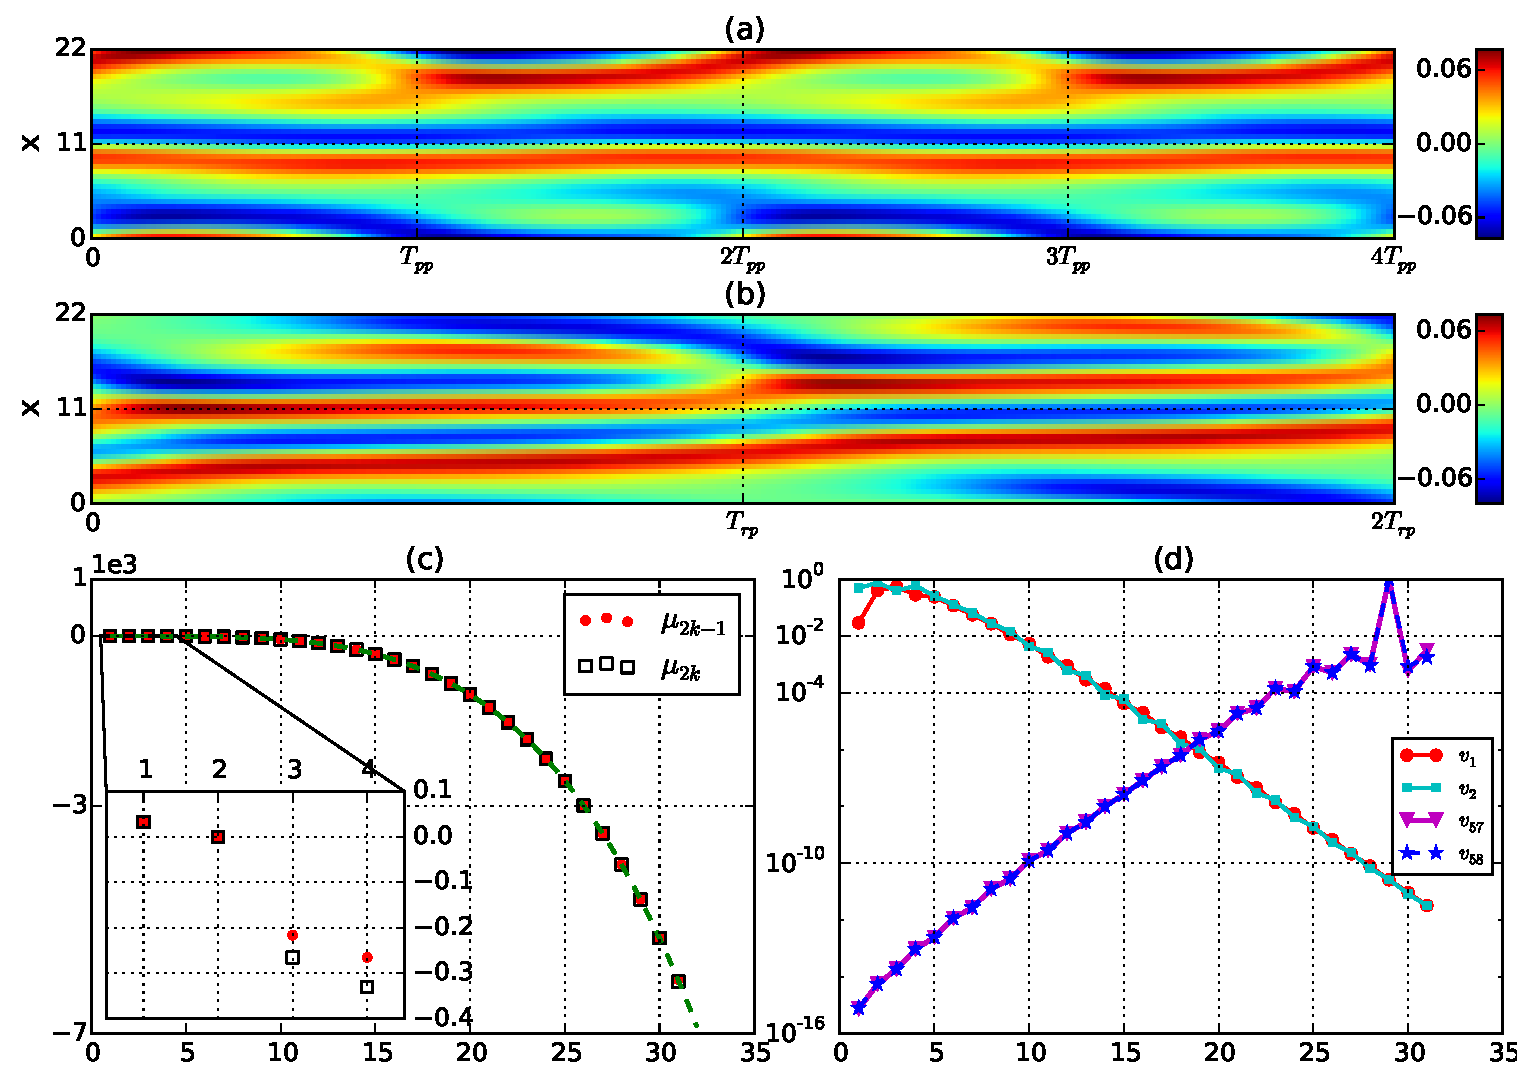
\includegraphics[width=0.9\linewidth]{pprpfigure}
  \caption{(Color online)
   (a) Pre\po\ $\cycle{pp}_{10.25}$ and
   (b) \rpo\ $\cycle{rp}_{16.31}$ in the full \statesp\ for total time
   $4\,\period{pp}$ and $2\,\period{rp}$, respectively. The phase shift
   for $\cycle{rp}_{16.31}$ after one prime period $\simeq-2.863$.
   (c) The real parts of Floquet exponents paired for a given $k$ as
   $(k,\eigRe[2k-1])$ and $(k,\eigRe[2k])$, for $\cycle{pp}_{10.25}$ with
   truncation number $N=64$. The dashed line (green) is
   $q_{k}^{2}-q_{k}^{4}$, with $x$-axis the indices of Fourier modes
   $k=1,2,\cdots,N/2-1$. The inset is a magnification of the region
   containing the 8 leading {\entangled} modes. As can be seen in
   \reftab{tab:floquet_ppo1}, for modes that follow, $k\geq 5$,
   the exponents are much smaller, in
   agreement with the expected separation into {\entangled} and
   {isolated} modes of \refref{YaTaGiChRa08}. For large
   indices, Floquet exponents
   appear in pairs corresponding to the real and imaginary
   part of Fourier modes.
   (d) The magnitudes of the Fourier components $|a_k| =
   |b_k+1i*c_k|$ of the 1st, the 2nd, the 57th and 58th \Fv s
   $\jEigvec[k]$ for $\cycle{pp}_{10.25}$ at initial time $\zeit =0$,
   truncation number $N=64$. For {\entangled} modes the first 4 Fourier
   are comparable in magnitude. For the $k_{th}$ isolated modes pair, the
   amplitude is concentrated on $k_{th}$ Fourier mode. The $x$-axis is
   labeled by the Fourier mode indices. Only the $k>0$ part is shown, the
   negative $k$ follow by reflection.
   }
  \label{fig:ppo1state}
\end{figure}

\begin{table}[h]
  \footnotesize
  \centering
  \caption{
    The first 10 and last four Floquet exponents and
    Floquet multiplier phases,
    $ \ExpaEig_i= \exp(\period{}\,\eigRe[i] \pm i\theta_{i})$, for
    orbits $\cycle{pp}_{10.25}$ and $\cycle{rp}_{16.31}$, respectively.
    $\theta_{i}$ column lists either the phase,
    if the Floquet multiplier is complex, or `-1' if the
    multiplier is real, but inverse hyperbolic. Truncation number
    $N=64$.
    The $8$ leading exponents correspond to the {\entangled} modes:
    note the sharp drop in the value of the $9_{th}$ and subsequent
    exponents, corresponding to the {isolated} modes.
  }
  \label{tab:floquet_ppo1}
  \begin{tabular}{l l c | l l c}
    \multicolumn{3}{c |}{$\cycle{pp}_{10.25}$} & \multicolumn{3}{c}{$\cycle{rp}_{16.31}$}\\
    $i$ & ~~~~~$\eigRe[i]$  & $\theta_{i}$  & $i$ & ~~~~~$\eigRe[i]$ & $\theta_{i}$  \\
    \hline
    1,2 & ~0.033209  &    $\pm$2.0079  &  1 &     ~0.32791  &              \\
    3 & -4.1096e-13  &                 &  2 &   ~2.8679e-12  &              \\
    4 & -3.3524e-14  &    -1           &  3 &   ~2.3559e-13  &              \\
    5 &  -0.21637    &                 &  4 &     -0.13214  &        -1    \\
    6,7 &  -0.26524  &   $\pm$2.6205   &  5,6 &   -0.28597  & $\pm$2.7724  \\
    8 &  -0.33073    &    -1           &  7 &     -0.32821  &       -1     \\
    9 &  -1.9605    &                  &  8 &      -0.36241  &             \\
    10 & -1.9676    &    -1            &  9,10 &   -1.9617  &  $\pm$2.2411 \\
    $\cdots$ &  $\cdots$    & $\cdots$ & $\cdots$ & $\cdots$ & $\cdots$   \\
    59 &  -5313.6   &    -1           &  59 &   -5314.4 &                 \\
    60 &  -5317.6   &                 &  60 &   -5317.7 &                 \\
    61 &  -6051.8   &    -1           &  61 &   -6059.2 &                 \\
    62 &  -6080.4   &                 &  62 &   -6072.9 &                 \\
    \hline
\end{tabular}
\end{table}
\begin{figure}[h]
  \centering
  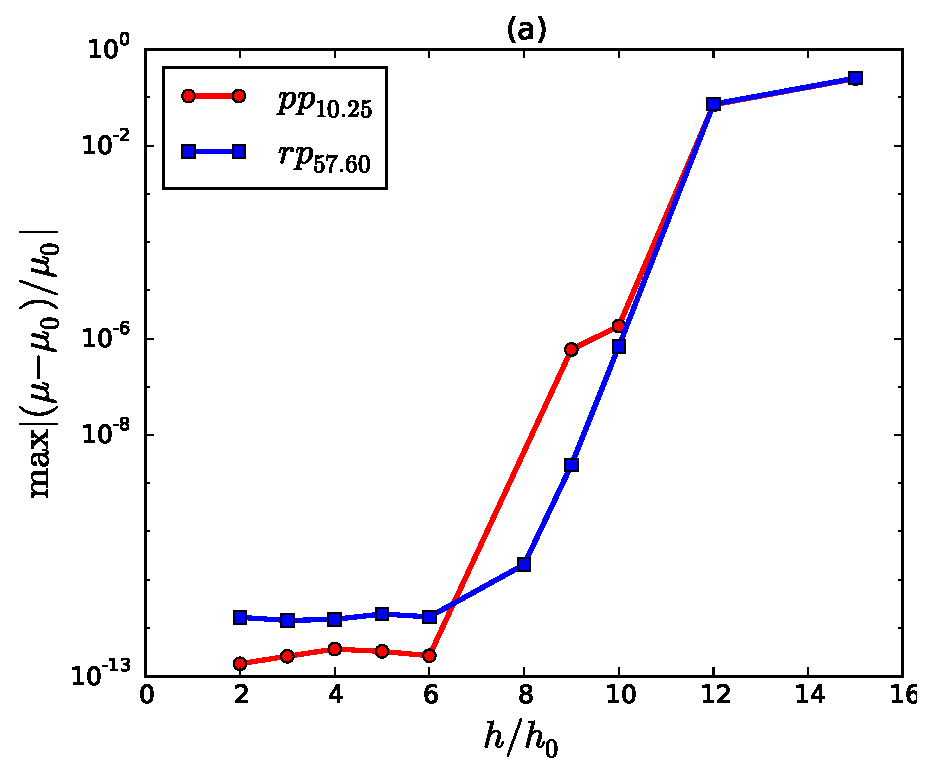
\includegraphics[width=0.47\linewidth]{ppo1FEerror} \hfill
  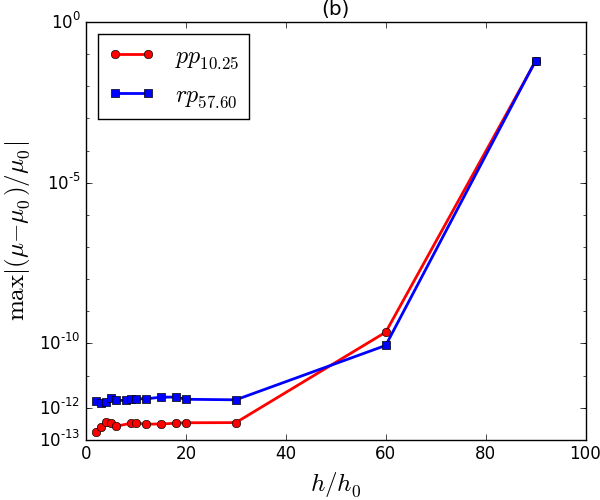
\includegraphics[width=0.47\linewidth]{rpo22FEerror}
  \caption{(Color online) Relative error of the real part of
    Floquet exponents associated with different time steps
    with which the Floquet matrix is integrated. Two orbits $\cycle{pp}_{10.25}$
    and $\cycle{rp}_{57.60}$ are used as an example with the base
    case $h_0 \approx 0.001$. (a) The maximal relative difference of
    the whole set of Floquet exponents with increasing time step (decreasing
    the number of ingredient segments of the orbit). (b) Only consider
    the first 35 Floquet exponents.}
  \label{fig:FEerror}
\end{figure}
\begin{figure}[h]
  \centering
  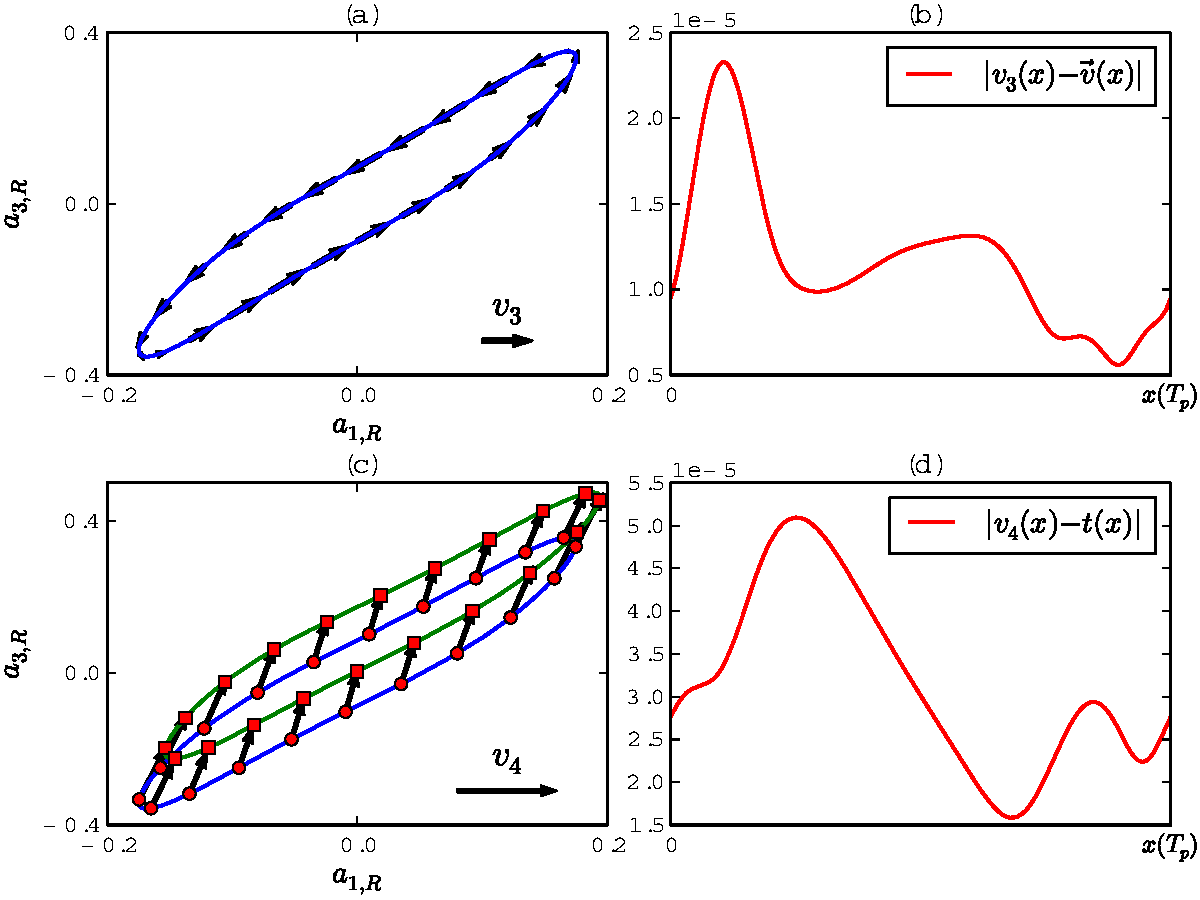
\includegraphics[width=1.0\linewidth]{ppo1vectfield}
  \caption{(Color online)
    Marginal vectors and the associated errors.
    (a) $\cycle{pp}_{10.25}$ in one period projected onto $[a_{1},b_{1},a_2]$
    subspace (blue curve), and its counterpart (green line) generated by
    a small group transformation $g(\ell)$
    , here arbitrarily set to $\ell= \,L/(20\pi)$. Magenta and black
    arrows represent the first and the second marginal \Fv s
    $\jEigvec[3](x)$ and $\jEigvec[4](x)$ along the prime orbit.
    (b) The solid red curve is the magnitude of the difference between
    $\jEigvec[3](x)$ and the velocity field $\vec{v}(x)$ along the orbit,
    and blue dashed curve is the difference between $\jEigvec[4](x)$ and
    the group tangent $t(x)=\mathbf{T}x$.
  }
  \label{fig:ppo1vectorfield}
\end{figure}


Stability analysis of \eqva\ is crucial for understanding the the geometry of
state space\rf{guckb}, but it is difficult for unstable \po s
due to lack of efficient and accurate numerical algorithms.
Floquet theorem says that
the Floquet matrix evaluated along a \po\ can be decomposed
as a product of a periodic matrix and an exponential matrix. We are interested
in the eigenvalues (Floquet multipliers) and the corresponding eigenvectors
(\Fv s) of the exponential matrix. More specifically,
define a flow $x(t) = f^t(x(0))$ generated by velocity field $\dot{x} = v(x)$
with $x$ a state vector. The evolution of perturbation along any orbit
is governed by the Jacobian of this flow
$J^t(x) = \partial f^t(x) / \partial x$, that is
$\delta x(t) = J^t(x) \delta x(0) $, and Jacobian itself is evolved as follows,
\begin{equation}
  \label{eq:jacobian}
  \frac{dJ^t(x)}{dt} = A(x)J^t(x)\,,\quad A(x) = \frac{v(x)}{x}
  \,.
\end{equation}
For a \po\ $x(T_p)=x(0)$,
the solution of \eqref{eq:jacobian}
for one period  $J_p = J^T(x(0))$ is called Floquet matrix or monodromy matrix.
$J_p e_i = e^{T(\eigRe[i]+\eigIm[i])} e_i$ gives the average expansion/contraction
rate $\eigRe[i]$ and
invariant directions $e_i$ in the tangent space.

For high dimensional nonlinear systems, Floquet exponents usually span a large
number of orders, so one period integration of \eqref{eq:jacobian} usually
results in a highly ill-conditioned Jacobian matrix, so we need to conduct
transformations on each short-time Jacobian since whole matrix can be decomposed
into the product of a sequence of square matrix. This is the basic idea of
\emph{\ped}, and it is based on the idea on \cLv\ algorithm and
\psd\ algorithm introduced in sec.~\ref{subsec:CAPSD}. See
\rf{DingCvit14} for the implementation details. Here, we only show the result
with 1-dimensional \KSe\ defined on a periodic domain.
\begin{equation}
u_t+\frac{1}{2}(u^2)_x+u_{xx}+u_{xxxx}=0\,,\; x\in [0,L]
\label{eq:ks}
\end{equation}
Here domain size $L=22$.
\KSe\ is equivariant under reflection and space translation: $-u(-x,t)$ and
$u(x+l,t)$ are also solutions if $u(x,t)$ is a solution.
Based on the consideration of these symmetries,
we focus on two types of orbits:
pre\po s $\hat{u}(0)=R\hat{u}(\period{p})$  and \rpo,
$\hat{u}(0)=g_p\hat{u}(\period{p})$. Here $R$ and $g_p$ are reflection and
rotation respectively.

At each repeat of the prime period, $\cycle{pp}_{10.25}$ is invariant
under reflection along $x=L/2$, \reffig{fig:ppo1state}\,(a), and
$\cycle{rp}_{16.31}$ has a shift along the $x$ direction as time goes on,
\reffig{fig:ppo1state}\,(b). Since $\cycle{pp}_{10.25}$ and
$\cycle{rp}_{16.31}$ are both
time invariant and equivariant under SO(2) group transformation $g(l)$,
there should be two marginal Floquet exponents, corresponding to the
velocity field and group tangent respectively.
\refTab{tab:floquet_ppo1} shows that the $2_{nd}$ and $3_{rd}$,
respectively $3_{rd}$ and $4_{th}$ exponents of $\cycle{rp}_{16.31}$,
respectively $\cycle{pp}_{10.25}$, are marginal, with accuracy as low as
$10^{-12}$, to which the inaccuracy introduced by the error in the closure of
the orbit itself also contributes.

In practice, caution should be
exercised when trying to determine the optimal number of time increments
that the orbit should be divided into. Here we determined satisfactory $m$'s by numerical
experimentation shown in \reffig{fig:FEerror}. Since larger time step means
fewer time increments of the orbit, a very small time step ($h_0 \approx 0.001$)
is chosen as the base case, and it is increased to test whether the
corresponding Floquet exponents change substantially or not. As shown in
\reffig{fig:FEerror} (a), up to $6h_0$ the whole Floquet spectrum varies within
$10^{-12}$ for both $\cycle{pp}_{10.25}$ and $\cycle{rp}_{57.60}$. These
two orbits represent two different types of invariant solutions which have
short and long periods, so we presume that time step $6h_0$ is good enough
for other short or long orbits too. On the other hand, if only the first
few Floquet exponents are desired, the time step can be increased further
to fulfill the job. As shown in \reffig{fig:FEerror} (b), if we are only
interested in the first 35 Floquet exponents, then time step $30h_0$ is small
enough. In high dimensional nonlinear systems, dynamics in the very contracting
directions is, very the often, decoupled from the physical modes, and shed little
insight into the system properties, so large time step could to used in order to
save time.
\refTab{tab:floquet_ppo1} and
\reffig{fig:ppo1state}\,(c) show that \psd\ is capable of resolving
Floquet multipliers differing by thousands of orders:
when $N=64$, the smallest Floquet multiplier  for $\cycle{pp}_{10.25}$ is
$|\ExpaEig_{62}| \simeq e^{-6080.4\times 10.25}$.

The two marginal directions have a simple geometrical interpretation.
\refFig{fig:ppo1vectorfield}\,(a) depicts the two marginal vectors of
$\cycle{pp}_{10.25}$ projected onto the subspace spanned by $[a_1, b_{1}, a_{2}]$
(the real, imaginary parts of the first mode and the real part of the
second Fourier mode). The first marginal eigen-direction (the $3_{rd}$
\Fv\ in  \reftab{tab:floquet_ppo1}) is aligned with the velocity
field along the orbit, and the second marginal direction (the $4_{th}$
\Fv) is aligned with the group tangent. The numerical
difference between the unit vectors along these two marginal directions
and the corresponding physical directions is shown in
\reffig{fig:ppo1vectorfield}\,(b). The difference is under $10^{-9}$ and
$10^{-11}$ for these two directions, which demonstrates the accuracy of
the algorithm.



\subsection{Local description of inertial manifold by \Fv s}
\label{subsec:LDIM}
Dissipative nonlinear systems described by partial differential equations
are infinite dimensional in principle, but for a lot of them, there exists
a finite dimensional inertial manifold and the dynamics is contained in it
after a transient period of evolution. Here we try to explain the concept of
``\emph{slaving}'' to understand how transition from infinite dimensional
space into finite dimensional subspace happens. For strict
mathematical treatment, see\rf{ Robinson1995, infdymnon}. Let $u$ be a dynamical
system in a finite or infinite dimensional Hilbert space $H$ governed by
\begin{equation}
  \label{eq:proto}
  \frac{du}{dt} + Au + f(u) = 0
\end{equation}
Assume this system has a n-dimensional inertial manifold, and
denote the projection from $H$ to the first $n$ eigenvectors of $A$ by
$P$. Let $Q = I - P$, then project \eqref{eq:proto} onto this subspace,
we obtain
\begin{equation}
  \label{eq:projected}
  \frac{dp}{dt} + Ap + Pf(p+\Phi(p)) = 0
\end{equation}
Here $p = Pu$ and $\Phi:PH\mapsto QH$. So we have reduced the dynamics to
a subspace given the existence of such a mapping $\Phi$, and the graph
of $\Phi$ is the inertial manifold. Equation \eqref{eq:projected} is
called the \emph{inertial form} of this system. Essentially, the existence
of inertial manifold indicates that the eigenmodes of $A$ with index larger than
$n$ is slaved to its first $n$ eigenmodes. For example, in \KSe,
eigenmodes of $A$ are Fourier modes, so short waves are slaved to long waves.
Anyway, inertial manifold can be interpreted in different ways, but the essential
idea is similar. See\rf{man90b} for an adiabatic illustration by a simple two
variable system.

To Approximate inertial manifold, or equivalently, to approximate
mapping $\Phi:PH\mapsto QH$ requires the knowledge of its exact dimension.
At present, people use empirical or some test number to truncate the
original system. For example, in \rf{foias88}, 3 modes are
used to represent the inertial manifold of 1-dimensional \KSe, but this
truncated model is not enough to preserve the bifurcation diagram. On the other
hand, mathematical upper bound for the dimension is not always tight.
However, as stated in
sec.~\ref{subsec:IM}, Recent progress in the numerical algorithm of \cLv s enables us
to expand tangent spaces into invariant subspaces.
\CLv s computed along long ergodic
trajectories are disentangled between the physical subspace and the transient
subspace, which serves as a criteria for determining the effective dimension
of the state space. This approach is different from the nonlinear Galerkin method
since it has no ambition to use a static set of eigenvectors to describe the dynamics,
it uses invariant vectors in the tangent space to linearly approximate the
inertial manifold locally.
From our intuition, we expect \Fv s along \po s can give the same dimension
of inertial manifold as \cLv s. Moreover, \Fv s seem more suitable for this job.
First, we have an efficient and accurate algorithm for calculating \Fv s
introduced in sec~\ref{subsec:PE}, and do not
need to follow an ergodic trajectory for a long time as \cLv\ algorithm does.
Second, \po s are dense on the strange attractor and probably only a
small subset of them is enough to represent the whole hierarchy in the system
if the symbolic dynamics of this system is known, so
experiments can be restricted to small number of short \po s.
But \cLv s along ergodic trajectories reveals little information about the
geometry of the strange attractor.


\paragraph{Angle distribution between physical and transient subspaces}
Like the experiments conducted in\rf{TaGiCh11, YaTaGiChRa08}, we measure the
angle between subspaces spanned by disjoint \Fv s along \po s inside
the 1-dimensional \KSe\ with domain size $L=22$.
Since symbolic dynamics in this system is unknown, we choose to do the statics
for all the \po s available to us with period $T<120$.
\begin{figure}[h]
  \centering
  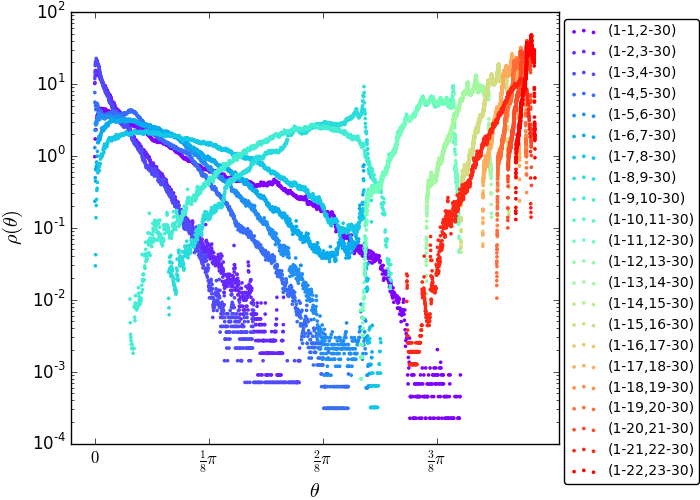
\includegraphics[width=0.48\textwidth]{angle120ppoSpace1} \hfill
  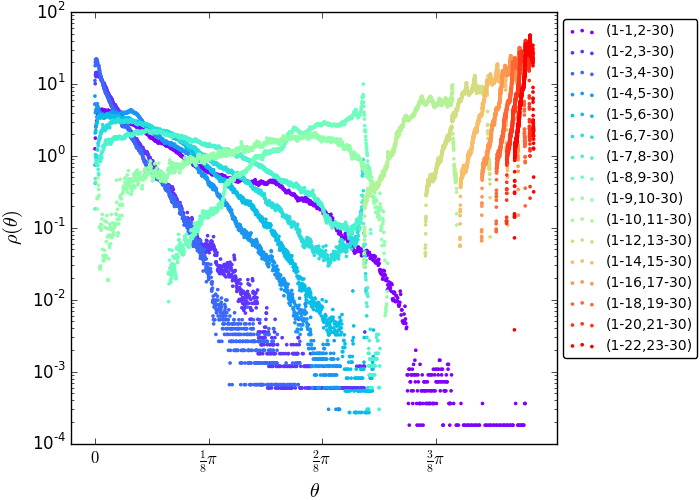
\includegraphics[width=0.48\textwidth]{angle120rpoSpace1}
  \caption{Angle distribution $\rho(\theta)$ versus $\theta$
    for \cycle{ppo} (left) and \cycle{rpo} which has $ T < 120$.
  }
  \label{fig:angDist}
\end{figure}
As shown in \reffig{fig:angDist}, we are measuring the distribution of
the angle between invariant subspace spanned by the first $k$ \Fv s
and the subspace spanned the
remaining $30-k$ \Fv s. Start from $k=1$, As we add more into
the first subspace, the possibility keeps nonzero until $k = 9$, and after
which, the distribution shrinks away from zero. The same qualitative
distribution is obtained for both pre-\po s and \rpo s.
Therefore, the first 8 \Fv s are entangled with each other and are
disentangled from the remaining set. We call the first set physical
\Fv s and the latter unphysical one. The unphysical set has little effect
on the dynamics in the neighborhood of this \po\ since all theses directions
are contracting, and thus small perturbation inside it will die out eventually.
So clearly, the first 8 \Fv s are enough to approximate the inertial manifold
at the neighborhood of all the \po s concerned in this
experiment and we expect that such threshold number
will not
change if we can find more \po s.
Since \po s are dense on the attractor, we expect the same number
apply to the whole inertial manifold.

\paragraph{difference vectors spanned by subset of \Fv s}
Ergodic trajectories are attracted by \po s along their stable directions,
and repelled by their unstable directions. Each unstable direction is
important since it determines how the system is stretched; however, if the
inertial manifold exists, then only a subset of the stable directions
have an effect on the dynamics asymptotically. So we believe that an ergodic
trajectory is moving in a subspace which is spanned by the set of
all unstable \Fv s and a subset of stable \Fv s around a \po\ locally.
So, the number of \Fv s used to span such a subspace can be regarded
as the dimension of inertial manifold.
\begin{figure}[h]
  \centering
  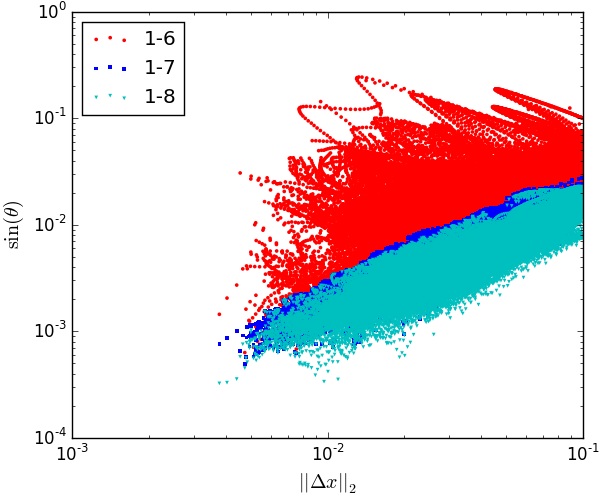
\includegraphics[width=0.48\textwidth]{ppo3truncated} \hfill
  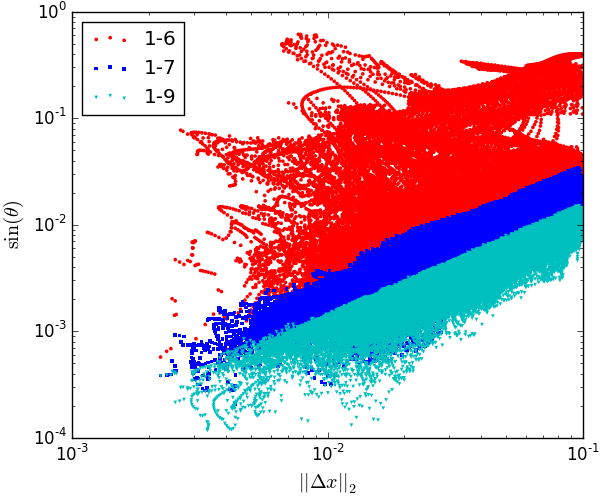
\includegraphics[width=0.48\textwidth]{rpo4truncated}
  \caption{
    scatter plot of $sin\theta$ vs the norm of difference vector.
    $\theta$ is the angle between $\Delta x$ and the subspace spanned
    by a subset of \Fv s.
    (a) $\cycle{ppo}_{32.36}$ with 198 shadowing incidences.
    (b) $\cycle{rpo}_{34.64}$ with 230 shadowing incidences.
  }
  \label{fig:angApproach}
\end{figure}

We borrow the idea from\rf{YaRa11} and conduct a set of experiments.
We generate a long ergodic trajectory and try to find incidences that it shadows
a specific \po. For each shadowing point $x$ on the ergodic trajectory,
we locate the nearest point $x_p$ on the \po\ to it and defined the
difference vector by $\Delta x = x - x_p$. When the orbit approaches or leaves the
\po, the difference vector is mainly controlled by the stable and unstable \Fv s,
so if we try to expand $\Delta x$ using a subset of \Fv s and see
how many of \Fv s is enough for a faithful expansion, we could almost get a
faithful approximation of the inertial manifold locally. In
\reffig{fig:angApproach}, if more than 7 \Fv s are used, then the
tendency shows that $\theta$ will
diminish to zero linearly as $\Delta x$ goes to zero, which is not true
if no more than 6 \Fv s are used to span the subspace. Note the experiments are
conducted in the symmetry-reduced state space, so the dimension of inertial
manifold of the full state space is $7+1$, which is consistent with the previous
result.

\subsection{Traveling wave in \cqcGLe}
In \cqcGL\ \eqref{eq:cqcgl1d}, traveling wave (\reqv) is defined as
a solution of
\[
A(x, 0) = e^{i\phi}A(x+ct, t)
\]
which is
\begin{equation}
  a_k(0) = e^{i\omega_\rho t}e^{ik\omega_\tau t}a_k(t)
  \label{eq:travelWaveFourier}
\end{equation}
in Fourier space.
Here $\omega_\rho$ is the velocity in the group tangent of phase
invariance symmetry: $\phi = \omega_\rho t$, and $\omega_\tau= 2\pi/L\cdot c$.
Levenberg-Marquardt algorithm is implemented to solve \eqref{eq:travelWaveFourier}
with random initial conditions. Dozens of {\reqva} are founded and a few
are shown in \reffig{fig:cqcglReqSet}.
Some of them are extensive spanning the whole domain; others are localized.
\begin{figure}[h]
  \centering
   (1)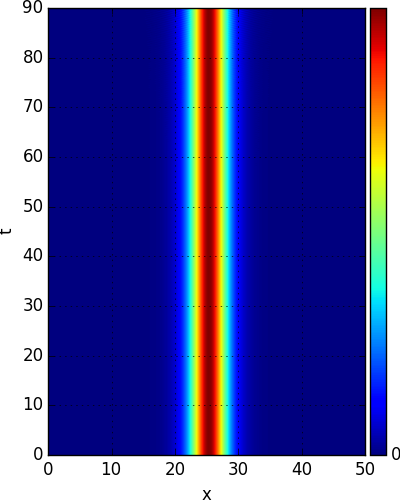
\includegraphics[width=.19\textwidth]{cqcglReq1T90}
   (2)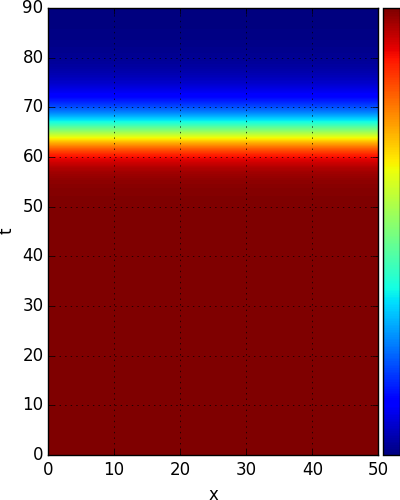
\includegraphics[width=.19\textwidth]{cqcglReq2T90}
   (3)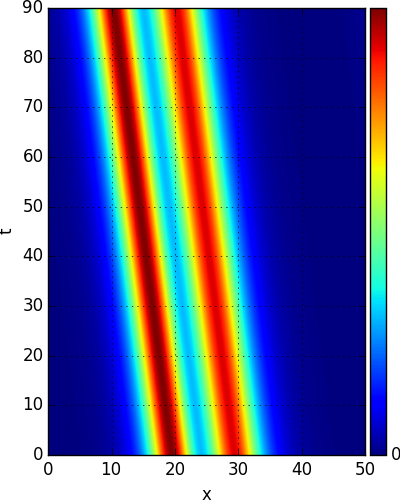
\includegraphics[width=.19\textwidth]{cqcglReq3T90}
   (4)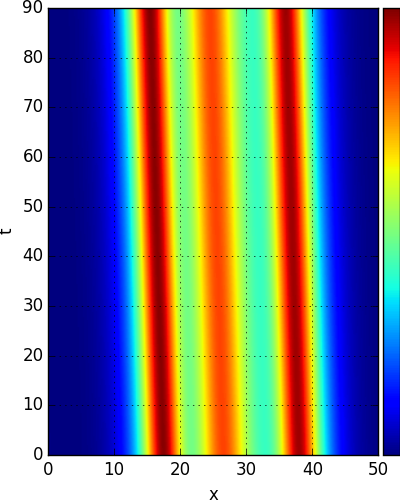
\includegraphics[width=.19\textwidth]{cqcglReq4T90}\\
   (5)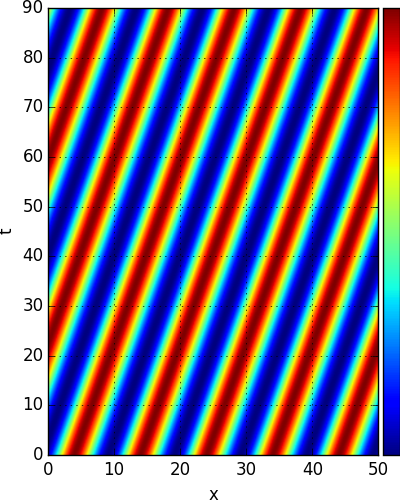
\includegraphics[width=.19\textwidth]{cqcglReq5T90}
   (6)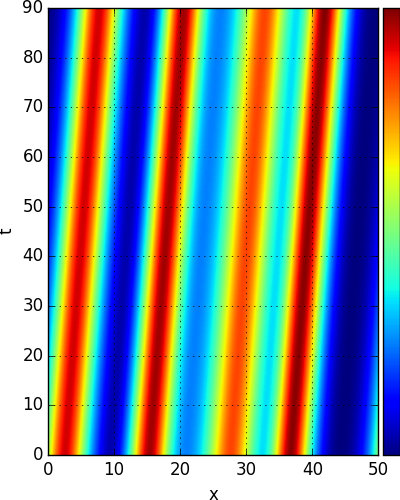
\includegraphics[width=.19\textwidth]{cqcglReq6T90}
   (7)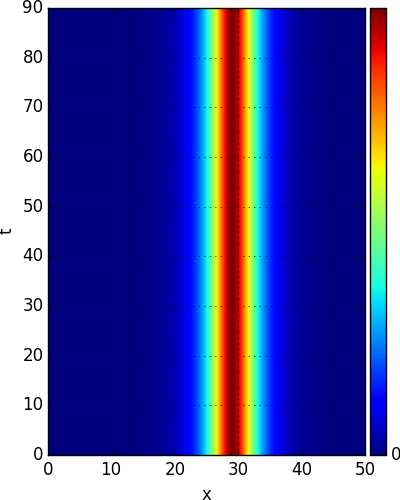
\includegraphics[width=.19\textwidth]{cqcglReq7T90}
   (8)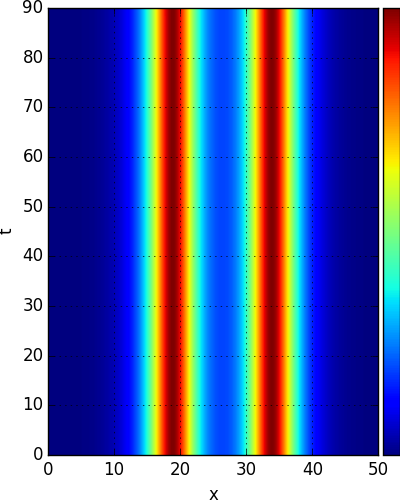
\includegraphics[width=.19\textwidth]{cqcglReq8T90}
  \caption{
    A set of different relative \eqva. (1) is different from
    (7) by the phase velocity. Plane wave solutions like (2) appear
    most frequently, and there is a set of solutions like (2) with
    different phase velocities and translational velocities.
    Only one representative is shown here.
  }
  \label{fig:cqcglReqSet}
\end{figure}
Here I are only interested in the one related to the soliton
(1) shown in
\reffig{fig:req1Config}. This {\reqv} has group velocity
$\omega_\tau = 0$ and $\omega_\rho=17.6675$.
\refFig{fig:req1Config} shows the profile of this \reqv\ and
its stability exponents. \refTab{tab:req1Stability} gives
the numerical values of these exponents.
\begin{table}
  \centering
  \begin{tabular}{c | c}
    index & $\lambda$ \\
    \hline
     1,2    &    0.1474653 $\pm$      17.2375582i\\
     3,4    &    0.1474643 $\pm$      17.2375572i\\
     5    &    -7.21620620e-14             \\
     6    &     -1.86242571e-13  \\
     7,8    &   -0.1002241 $\pm$      17.6645298i\\
     9,10    &   -0.1008975 $\pm$      17.6556189i\\
     \hline
  \end{tabular}
  \caption{The first 10 stability exponents of {\reqv}
   \reffig{fig:req1Config}.
 }
  \label{tab:req1Stability}
\end{table}
\begin{figure}[h]
  \centering
  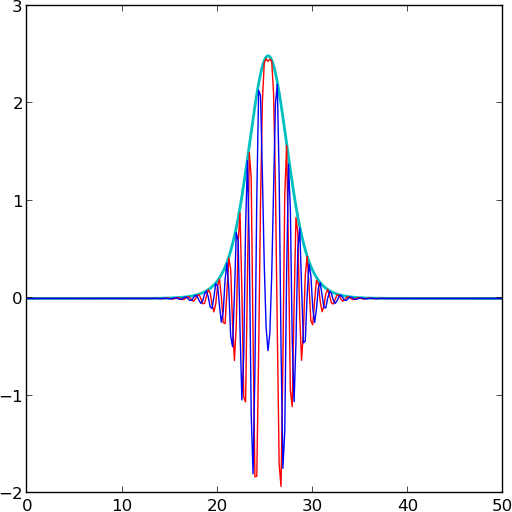
\includegraphics[width=0.35\textwidth]{req1Config} \hfill
  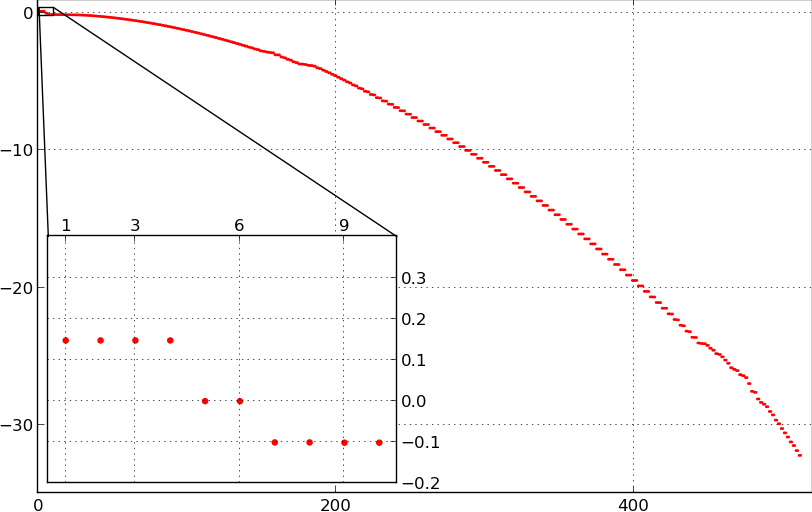
\includegraphics[width=0.55\textwidth]{req1Stability}
  \caption{(Left panel) Spatial profile of the {\reqv} (1) at some
  instant, and the real parts of the spectrum of stability exponents of
  this {\reqv}. The green line is the magnitude of the {\reqv}. Red and
  blue lines are respectively its real and imaginary parts.
  (Right panel) Stability spectrum.
  }
  \label{fig:req1Config}
\end{figure}

There are two marginal directions, which correspond to the group tangents
of translational symmetry and phase invariance. Note the velocity field
lies in this two dimensional subspace.
Four unstable directions are in two conjugate pairs, with almost
the same expansion rates. The corresponding eigenvectors have
almost the same profile.
    \PC{2015-09-06
    We had explained in the blog why exponents come in `almost' quadruplets.
    Is it worth including that here? In any case, that must go into the
    thesis.
    }
Also, the profile is slightly asymmetric
as shown in \reffig{fig:req1eigenvectors}(a)(b).
On the other hand, since
this system has reflection symmetry. The real/imaginary part of the
leading eigenvector of the reflected state is shown in
\reffig{fig:req1eigenvectors}(c)(d). The left side is larger than
the right side for this reflected state.
\begin{figure}[h]
  \centering
  (a)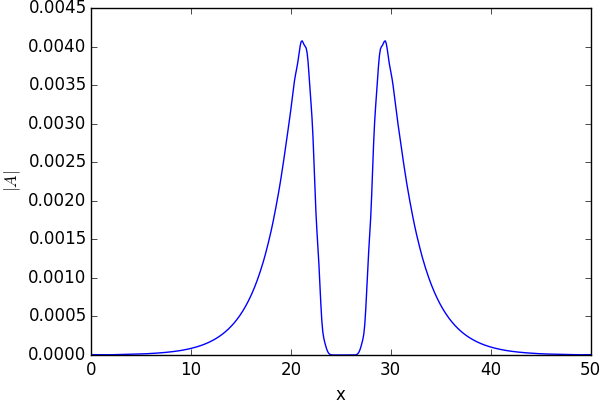
\includegraphics[width=0.46\textwidth]{cqcglReq1V1Real}
  (b)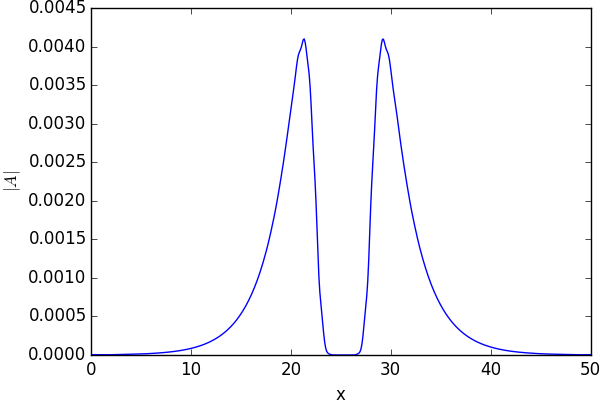
\includegraphics[width=0.46\textwidth]{cqcglReq1V1Imag} \\
  (c)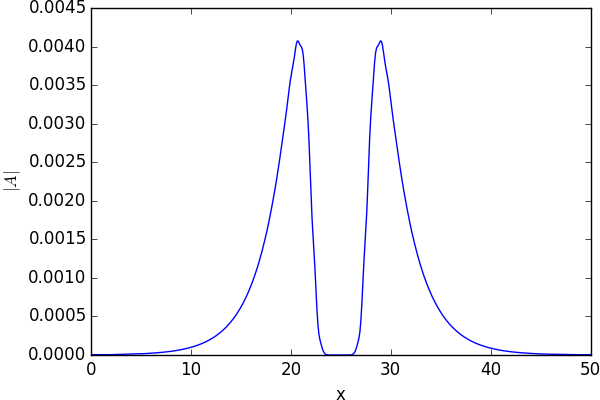
\includegraphics[width=0.46\textwidth]{cqcglReq1ReflectV1Real}
  (d)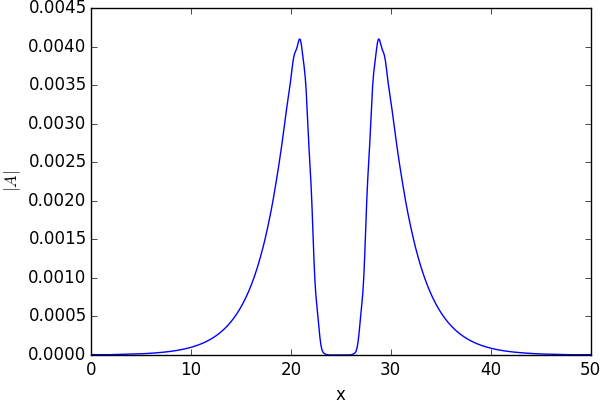
\includegraphics[width=0.46\textwidth]{cqcglReq1ReflectV1Imag}
  \caption{
    Eigenvectors of the {\reqv}.
    (a)(b) the magnitude of the real/imaginary part of the 1st
    eigenvector of the relative equilibrium.
    (c)(d) The relative equilibrium is reflected $A(x)\to A(-x)$.
    The magnitude of the real/imaginary part of the 1st
    eigenvector of the reflected relative equilibrium.
  }
  \label{fig:req1eigenvectors}
\end{figure}
Note that the unstable directions have should profile and the
peaks are exactly at the place where explosion
happens. In this sense, explosions are just homoclinic connections of
this {\reqv}.

Actually, \refref{Akhmediev04} uses an approximation method to
approximate the unstable directions, and gets a symmetric and an asymmetric
solutions, which are used to explain the symmetric and asymmetric
explosions. Here we only got 4 slightly asymmetric solutions, but they have
reflection symmetry, which means that if there are perturbations at both
sides of the soliton, then symmetric explosion also could occur. Also
this is a pure numerical result. No approximation is used.

Next, I will investigate the unstable manifold of this {\reqv} to
see how the flow is organized around this \reqv. But before that,
we need to reduce all the symmetries mentioned in sec.~\ref{subsec:cqcgl}
and then work on the symmetry-reduced state space.

\paragraph{Reduce continuous symmetries} The two continuous symmetry
operations in
\cqcGL\ system can be regarded as one Lie group of two generators, since
these two symmetries commute.
$g(\theta,\phi) = g_\tau(\theta)g_\rho(\phi)$ produces translation in
Fourier space as
\beq
a_k(t) \to a_k(t)e^{i(k\theta + \phi)}
\ee{eq:ft}
In order to reduce this continuous symmetry,
we define a subspace on which all points has vanishing imaginary part
of the 1st and -1st modes
\[
Im(a_1) = Im(a_{-1}) = 0
\,,
\]
and transform all points in the full state space to
this subspace by $ \ssp(\tau) = \LieEl(\theta_s, \phi_s) \, \sspRed(\tau)$
with
\beq
\phi_s = \frac{1}{2}(\alpha_{1}+\alpha_{-1}) \,, \quad
\theta_s = \frac{1}{2}(\alpha_{1} - \alpha_{-1}) \,.
\ee{eq:cqcglPhaseAngle}
Here, $\alpha_{\pm 1}$ are the phase angle of $\pm 1$ mode.
Subscript s denotes the specific angle from slice to full state space.

On the other hand, this choice of slice introduces phase wrapping
problem. From \eqref{eq:cqcglPhaseAngle}, when $\alpha_1$ or
$\alpha_{-1}$ is wrapped, namely, jumps $2\pi$ suddenly, $\phi_s$ and
$\theta_s$ jumps $\pi$. Therefore, at this point, trajectory in the
slice is not continuous. More importantly, it also means that we have
introduced another discrete symmetry. Each orbit in the full state space
has 2 corresponding orbits in the slice, which are related by
$g(\pi, \pi)$. You can have a feeling of how well
slice works in \reffig{fig:cqcglReduceSymT75h005}

\begin{figure}[h]
  \centering
  \begin{subfigure}{.23\linewidth}
    \centering
    \captionsetup{justification=centering}
    \caption{}
    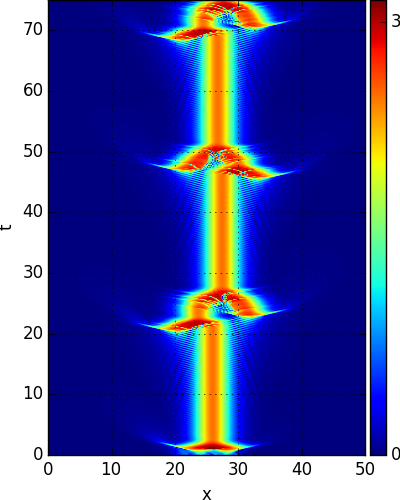
\includegraphics[width=\textwidth]{cqcglStateSpaceT75h005}
    \label{}
  \end{subfigure}
  \begin{subfigure}{.23\linewidth}
    \centering
    \captionsetup{justification=centering}
    \caption{}
    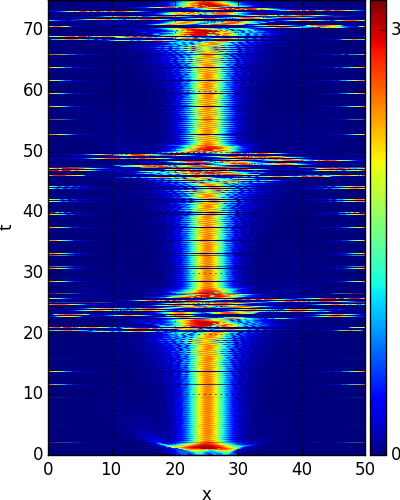
\includegraphics[width=\textwidth]{cqcglSliceWrappedT75h005}
    \label{}
  \end{subfigure}
  \begin{subfigure}{.23\linewidth}
    \centering
    \captionsetup{justification=centering}
    \caption{}
    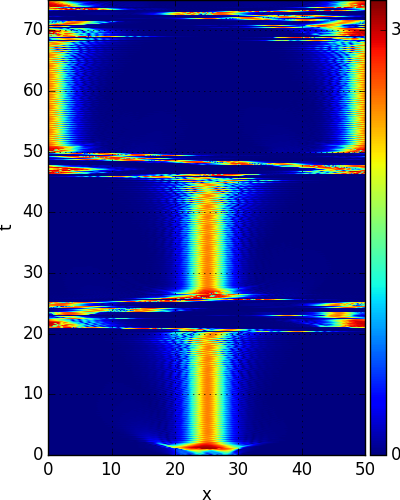
\includegraphics[width=\textwidth]{cqcglSliceUnwrappedT75h005}
    \label{}
  \end{subfigure}
  \begin{subfigure}{.23\linewidth}
    \centering
    \captionsetup{justification=centering}
    \caption{}
    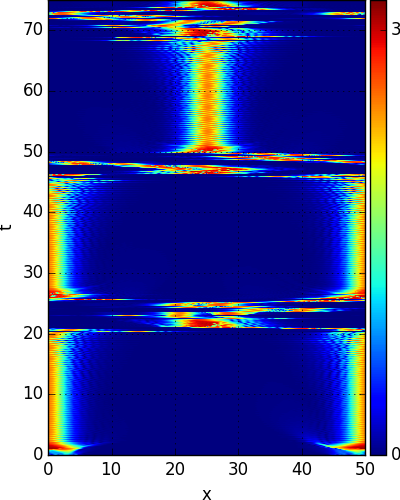
\includegraphics[width=\textwidth]{cqcglSliceUnwrappedShiftedT75h005}
    \label{}
  \end{subfigure}
  \begin{subfigure}{.23\linewidth}
    \centering
    \captionsetup{justification=centering}
    \caption{}
    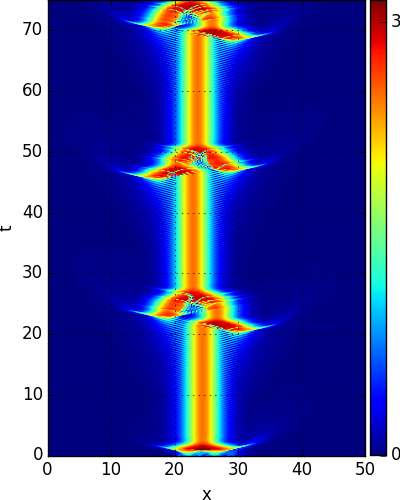
\includegraphics[width=\textwidth]{cqcglStateSpaceReflectT75h005}
    \label{}
  \end{subfigure}
  \begin{subfigure}{.23\linewidth}
    \centering
    \captionsetup{justification=centering}
    \caption{}
    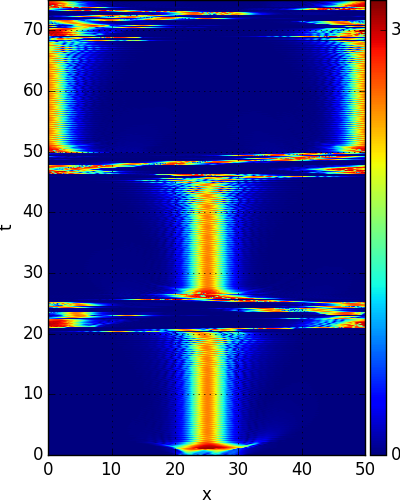
\includegraphics[width=\textwidth]{cqcglSliceUnwrappedReflectT75h005}
    \label{}
  \end{subfigure}
  \begin{subfigure}{.23\linewidth}
    \centering
    \captionsetup{justification=centering}
    \caption{}
    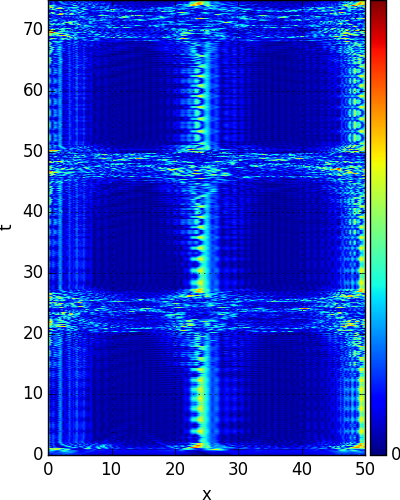
\includegraphics[width=\textwidth]{cqcglAllReduceT75h005}
    \label{}
  \end{subfigure}
  \caption{
    (a) Full state space trajectory.
    (b) Continuous symmetry reduced of (a) with wrapped phase.
    (c) Continuous symmetry reduced of (a) with unwrapped phase.
    (d) rotated by $g(\pi, \pi)$ of (c).
    (e) The reflected states of (a).
    (f) Continuous symmetry reduced of (e).
    (g) after reducing all symmetries of (a)(b).
  }
  \label{fig:cqcglReduceSymT75h005}
\end{figure}


\paragraph{Reduce reflection symmetry}
To illustrate the procedure of reducing reflection symmetry, we'd better split the
real and imaginary part the Fourier modes $a_k = b_k+ 1i*c_k$
and work on the state space defined by
\beq
[b_0, c_0, b_1, c_1, \cdots, b_{N/2-1}, c_{N/2-1},
b_{-N/2+1}, c_{-N/2+1}, \cdots, b_{-1}, c_{-1}]
\,,
\ee{eq:cqcglStateSpace}
Reflection symmetry ($a_k \to a_{-k}$) in state space \eqref{eq:cqcglStateSpace} is
\begin{equation}
(b_0, c_0, b_1, c_1, b_2, c_2, \cdots, b_{-1}, c_{-1})
  \Rightarrow
(b_0, c_0, b_{-1}, c_{-1}, b_{-2}, c_{-2}, \cdots, b_{1}, c_{1})
  \label{eq:reflectFullStateSpace}
\end{equation}
Our strategy is reducing continuous symmetries first, then reducing reflection symmetry.
Inspecting \eqref{eq:reflectFullStateSpace}, you find that
a state point in slice under reflection is still in the slice.
You can analogize it to
the case in a 3-d space: we choose a 2-d plane slice which is perpendicular
to the reflection axis. Therefore, a point in slice will be reflected to another
point in the slice by the original reflection operation. This is the exact reason
for the choice of this specific slice.

Now we try to reduce symmetry \eqref{eq:reflectFullStateSpace}. We take a 3-step
approach. First perform a linear transformation
\begin{align}
& (b_0, c_0, b_1, c_1, b_2, c_2, \cdots, b_{-1}, c_{-1})
  \Rightarrow \nonumber \\
& (b_0, c_0, \frac{b_1-b_{-1}}{2}, \frac{c_1-c_{-1}}{2}, \frac{b_2-b_{-2}}{2},
  \frac{c_2-c_{-2}}{2}, \cdots,
  \frac{b_1+b_{-1}}{2}, \frac{c_1+c_{-1}}{2})
  \label{eq:reflectStep1}
\end{align}
Denote the transformed state as
$(b_0, c_0, p_1, q_1, \cdots, q_{N/2-1}, p_{-N/2+1}, \cdots, p_{-1}, q_{-1})$. So under reflection,
$p_i\,,q_i$ with $i<0$ keep unchanged, but $p_i\,,q_i$ with $i>0$ flip sign. In
the second stage, we perform a nonlinear transformation:
\begin{align}
& (b_0, c_0, p_1, q_1, p_2, q_2, \cdots, q_{N/2-1}, p_{-N/2+1}, \cdots, p_{-1}, q_{-1})
  \Rightarrow \nonumber \\
& (b_0, c_0, r_1, s_1, r_2, s_2, \cdots, s_{N/2-1}, p_{-N/2+1}, \cdots, p_{-1}, q_{-1})
  \label{eq:reflectStep2}
\end{align}
Here $p_i\,,q_i$ with $i<0$ are unchanged.
\[
r_1 = \frac{p_1^2-q_1^2}{\sqrt{p_1^2+q_1^2}}\,,
s_1 = \frac{p_1 q_1}{\sqrt{p_1^2+q_1^2}} \,,
r_2 = \frac{q_1 p_2}{\sqrt{q_1^2+p_2^2}} \,,
s_2 = \frac{p_2 q_2}{\sqrt{p_2^2+q_2^2}} \,,
\cdots
\]
The previous two steps reduce the reflection symmetry of original system
$a_k \to a_{-k}$; however, the specific choice of slice
introduces another reflection symmetry: even modes flip sign.
\begin{equation}
(b_0, c_0, b_1, c_1, b_2, c_2, \cdots, b_{-1}, c_{-1})
  \Rightarrow
(-b_0, -c_0, b_{-1}, c_{-1}, -b_{-2}, -c_{-2}, \cdots, b_{1}, c_{1})
  \label{eq:2ndReflection}
\end{equation}
Under representation \eqref{eq:reflectStep2}, this reflection turns to be
\begin{align*}
& (b_0, c_0, r_1, s_1, r_2, s_2, \cdots, s_{N/2-1}, p_{-N/2+1}, \cdots, p_{-1}, q_{-1})
  \Rightarrow \\
& (-b_0, -c_0, r_1, s_1, -r_2, s_2, \cdots, -r_{N/2-1}, s_{N/2-1},
  p_{-N/2+1}, q_{-N/2+1}, -p_{-N/2+2}, -q_{-N/2+2}, \cdots, p_{-1}, q_{-1})
\end{align*}
Terms $(b_0, c_0, r_2, \cdots, r_{N/2-1}, p_{-N/2+2}, q_{-N/2+2}, \cdots, p_{-2}, q_{-2})$
flip sign, so we can
utilize the same formulation to reduce this reflection symmetry:
\begin{equation}
(b_0, c_0, r_2, \cdots, r_{N/2-1}, p_{-N/2+2}, q_{-N/2+2}, \cdots, p_{-2}, q_{-2})
\Rightarrow
(t_1, t_2, \cdots, t_{N-2})
  \label{eq:reduce2ndReflection}
\end{equation}
\[
t_1 = \frac{b_0^2-c_0^2}{\sqrt{b_0^2+c_0^2}}\,,
t_2 = \frac{b_0 c_0}{\sqrt{b_0^2+c_0^2}} \,,
t_3 = \frac{r_2 c_0}{\sqrt{r_2^2+c_0^2}} \,,
t_3 = \frac{r_3 r_2}{\sqrt{r_3^2+r_2^2}} \,,
\cdots
\]

In conclusion, the following coordinate reduces all symmetries inside
this system.
\begin{equation}
  \label{eq:Finalssp}
  (t_1, t_2, r_1, s_1, t_3, s_2, \cdots, s_{N/2-1}, p_{-N/2+1}, \cdots, p_{-1}, q_{-1})
  \,.
\end{equation}

\refFig{fig:cqcglReduceSymT75h005} (g) shows the state after reducing all symmetries of
this system. When only continuous symmetry is reduced, (a),(e) become (c) and (f) respectively.
Note, (f) is exactly a reflection image of (c). If Reflection symmetries are reduced
further, (c) (d) (f) all turn to (g).

% siminos/xiong/thesis/proposal/tex/proposal.tex
% $Author: xiong $ $Date: 2015-09-03 13:21:45 -0400 (Thu, 03 Sep 2015) $

\section{Plan for future work}
\label{sec:future}

\subsection{Dimension of inertial manifold}
We have only tested the method described in sec.~\ref{subsec:LDIM}
to investigated the dimension of inertial manifold in
1-dimensional \KSe, but we think this method can be applied to
other turbulent systems as well, for example \cGLe, 2-d or 3-d
Navier-Stokes equation. The point we conduct such research to other
systems in the next step
 is that
usually the mathematical proof of existence of inertial manifold
sheds
limited information about its exact dimension. Moreover,
for systems like
3-d Navier-Stokes, the existence of inertial manifold is still
unknown, so the experiments investigating decoupling in the
tangent space by \Fv s can serve as a valuable tool to provide
accurate enough information about the local geometry of inertial
manifold ahead of strict mathematical statements.
Also, this information can help engineers to use the appropriate
resolution in the numerical turbulence simulation.

\subsection{Cycle expansions for \cqcGLe}
We have found quite a few \reqv s in 1-d \cqcGLe\ and converted
the dynamics into the symmetry-reduced space. The next step
is trying to find \po s or \rpo s inside this system and
hopefully build the symbolic dynamics according to the
geometry of this hierarchy of \po s.

with this set of \po s, cycle expansion can be applied to \Fd\
\eqref{Z(s)} with interesting physical quantity such as diffusion rate as
the observable. Therefore, our ultimate goal of studying \cqcGLe\ is to
give exact prediction about the long time behavior of soliton solution in
it. Also such method can be applied to the 2-d \cqcGL and analyze the
diffusion constant of the random walk reported in\rf{CaCiDeBr12}.


\newpage
\bibliographystyle{plain}    % Set the bibliography style. agu04, plain, alpha, etc.
\bibliography{../../bibtex/siminos}   % Use the BibTeX file ``References.bib''.

\end{document}
